\documentclass[a4paper,11pt,twoside,openright]{report}

% Use the preamble defined
%!TEX root = ../super_main.tex

% ========================================================= %
%         _____           _                         		% 
%        |  __ \         | |                                %
%        | |__) |_ _  ___| | ____ _  __ _  ___  ___ 		%
%        |  ___/ _` |/ __| |/ / _` |/ _` |/ _ \/ __|        %
%        | |  | (_| | (__|   < (_| | (_| |  __/\__ \        %
%        |_|   \__,_|\___|_|\_\__,_|\__, |\___||___/        %
%                                    __/ |                  %
%                                   |___/                   %
% ========================================================= %

% Margin
\usepackage[a4paper, inner = 4cm, outer = 2.4cm, top = 2.4cm, bottom = 2.4cm, pdftex]{geometry}

% Line numbering
\usepackage{lineno}

% 
\usepackage{filecontents}

% Colors packages
% Default colors can be found here http://en.wikibooks.org/wiki/LaTeX/Colors#The_68_standard_colors_known_to_dvips
\usepackage[usenames, dvipsnames]{xcolor} 
\usepackage{colortbl}
\definecolor{eclipse_blue}{RGB}{46,55,247}
\definecolor{eclipse_red}{RGB}{147,86,135}

% Language support
\usepackage[T1]{fontenc}
\usepackage[utf8]{inputenc}

% Used for making CFG 
% Rounded is to use EBNF
% Nounderscore is to use underscores in label names
\usepackage[rounded, nounderscore]{syntax}

% Used to make a directory Tree (CD content etc.)
\usepackage{dirtree}

% Fonts
\usepackage{lmodern}
\usepackage{courier}

% Use any font size
\usepackage{anyfontsize}

% Greek letters
\usepackage{textgreek}

% Used for making pretty math
\usepackage{amssymb}
\usepackage{amsmath}
\usepackage{stmaryrd}
\usepackage{upquote} % to use ^

% Adds pretty commas in math expressions
\usepackage{icomma}

% FiXme comments (fxnote)
\usepackage{fixme}

% Setup for the FiXme comments 
\fxsetup{
    status = draft,
    author = Comment,
    layout = footnote, % also try footnote or pdfnote
    theme = color
}

%todo setup
\usepackage[textwidth=2.0cm, textsize=small]{todonotes}
\setlength{\marginparwidth}{2cm}

% Graphics
\usepackage{graphicx}

% Captions (for figures etc.)
\usepackage[hang, footnotesize, bf]{caption}

% Used for making multiple figures within one figure
\usepackage{wrapfig}
\usepackage{subcaption}

% Custom styling for titles (chapter, section etc.)
\usepackage{titlesec}

% Special notation for appendix chapters
\usepackage[titletoc]{appendix}

% Used for floatbarriers
\usepackage{placeins}

% Used for double hlines
\usepackage{hhline}

% Used for \pdfbookmarks. Hidelinks will hide red boxes in some pdf-viewers.
\usepackage[bookmarks = true, hidelinks]{hyperref}

% Improved linebreaking
\usepackage{microtype}

% Used for tabels
\usepackage{booktabs}
\usepackage{rotating}

% Used for lists
\usepackage{enumerate}

% Header and footer on page
\usepackage{lastpage}
\usepackage{afterpage}
\usepackage{fancyhdr}

% Used for making multiple columbs
\usepackage{multicol}

% Used for making multiple rows
\usepackage{multirow}

% Used for generating lipsum text
\usepackage{lipsum}

% Used for making space after defined commands.
% This way we can write \command instead of \command{}.
\usepackage{xspace}

% Will show the name of the label in the margin (Uncomment to show labels)
% \usepackage[inline]{showlabels}

% Package used to make spacing between items in itemize and enumarations smaller.
\usepackage{enumitem}

% Makes it possible to embed PDF documents
\usepackage{pdfpages}


% ========================================================= %
% / / / / / / / / / / / / / / / / / / / / / / / / / / / / / %
% ========================================================= %



% ========================================================= %
%                _____       _ _   _       _ 				%
%               |_   _|     (_) | (_)     | |				%
%                 | |  _ __  _| |_ _  __ _| |				%
%                 | | | '_ \| | __| |/ _` | |				%
%                _| |_| | | | | |_| | (_| | |				%
%               |_____|_| |_|_|\__|_|\__,_|_|				%
%															%
% ========================================================= %

% Fixes some orphans (horeunger)
\widowpenalty = 300
\clubpenalty = 300

% All chapters must start on a new uneven page
\let\origdoublepage\cleardoublepage

\newcommand{\clearemptydoublepage}{
  \clearpage
  {\pagestyle{empty}\origdoublepage}
}
\let\cleardoublepage\clearemptydoublepage
\let\originalchapter=\chapter
\def\chapter{\cleardoublepage\originalchapter}

% Justification for captions
\captionsetup{justification = justified}

% Define graphics pack
\graphicspath{{graphic/}}

% Used for page header and footer
\pagestyle{fancyplain}
\fancyhf{}
\fancyhead[RO]{\slshape \rightmark}
\fancyhead[LE]{\slshape \leftmark}

% Set head height
\setlength{\headheight}{14.2pt}

%Set depth of toc to include sections
\setcounter{tocdepth}{1}

% ========================================================= %
% / / / / / / / / / / / / / / / / / / / / / / / / / / / / / %
% ========================================================= %



% ========================================================= %
%                 _____      _                				%
%                / ____|    | |               				%
%               | |     ___ | | ___  _ __ ___ 				%
%               | |    / _ \| |/ _ \| '__/ __|				%
%               | |___| (_) | | (_) | |  \__ \				%
%                \_____\___/|_|\___/|_|  |___/				%
%															%
% ========================================================= %

% Color used for fxnotes
\colorlet{fxnote}{Red}

% Primary color (Used for chapter headline etc.)
\colorlet{primarycolor}{Blue}

% ========================================================= %
% / / / / / / / / / / / / / / / / / / / / / / / / / / / / / %
% ========================================================= %                               



% ========================================================= %
%                   _____ _         _      					%
%                  / ____| |       | |     					%
%                 | (___ | |_ _   _| | ___ 					%
%                  \___ \| __| | | | |/ _ \					%
%                  ____) | |_| |_| | |  __/					%
%                 |_____/ \__|\__, |_|\___|					%
%                              __/ |       					%
%                             |___/        					%
% ========================================================= %

% Style for definitions
%!TEX root = ../../super_main.tex

% Packages used
\usepackage{amsthm}
\usepackage{thmtools}

% ================================================ %

% Style for the "definitionstyle" definition
\declaretheoremstyle
[
  spaceabove = \parsep, 
  spacebelow = \parsep,
  notebraces = {}{},
  headpunct = {},
  postheadspace = \newline,
  headformat = {{\NAME} {\NUMBER}:{\NOTE}},
  mdframed = {
    backgroundcolor = gray!15, 
    linecolor = gray!60,
    linewidth = 5pt,
    skipabove = 1em,
    skipbelow = 1em,
    innertopmargin = 0.7em,
    innerbottommargin = 0.7em,
    roundcorner = 0em,
    skipbelow = \parsep,
    skipbelow = \parsep,
    topline = false,
    bottomline = false,
    rightline = false,
  },
]
{definitionstyle}

% Declare a new theorem used for definitions
\declaretheorem
[
  style = definitionstyle,
  name = Definition,
  numberwithin = chapter,
]
{definition}

% Style for lstlistings (code snippets)
%!TEX root = ../../super_main.tex

% Packages used
\usepackage{listings}

% Package used to display pseudo code (algorithms)

\usepackage{algorithm}% http://ctan.org/pkg/algorithms
%\usepackage{algorithmic}
\usepackage{algpseudocode}% http://ctan.org/pkg/algorithmicx

% ================================================ %

\captionsetup[lstlisting]{
    format = listing
}

% Default style for all lstlistings
\lstset 
{
    backgroundcolor = \color{white},
    keywordstyle = \color{blue},
    commentstyle = \color{ForestGreen!80}\textit,
    stringstyle = \color{green}\textbf,
    basicstyle = \scriptsize\ttfamily\bfseries,
    numberstyle = \tiny,
    numbers = left,
    breaklines = true,
    breakatwhitespace=true,
    showstringspaces = false,
    tabsize = 3,
    captionpos = b,
    extendedchars = true,
    escapeinside = {//*}{\^^M}, % Use latex inside lstlistings. For instance for refferences.
    frame = tblr,
    backgroundcolor = \color{gray!5},
    xleftmargin = 3.5pt,
}

% Write "Code snippet" instead of "listing".
\renewcommand{\lstlistingname}{Code Snippet}

% General style for the whole lstlisting
\DeclareCaptionFormat{listing}{#1#2#3}
\captionsetup[lstlisting]{format = listing}

\lstdefinelanguage{TAInC} 
{
    morekeywords=[1]{number, boolean}, 
    keywordstyle=[1]\color{NavyBlue},
    morekeywords=[2]{do, if, else, run, when, startup, return, NAME},
    keywordstyle=[2]\color{Magenta},
    morekeywords=[3]{Tank, Gun, Battle},
    keywordstyle=[3]\color{Green},
    morekeywords=[4]{BattleEnded,BulletHit, BulletHitBullet, BulletMissed, Death, HitByBullet, HitTank, HitWall, TankDeath, RoundEnded, ScannedTank, Win},
    keywordstyle=[4]\color{Bittersweet},
    morekeywords=[5]{action, calculation},
    keywordstyle=[5]\color{Fuchsia},
    sensitive = true,
    morecomment = [l]{//},
    morecomment = [n]{/*}{*/}
}

% Custom lststyle named tainc
\lstdefinestyle{tainc}
{
    breaklines = true,
    columns = fullflexible,
    language = TAInC
}

% Custom lstinline for TAInC named taincinline
\newcommand{\taincinline}[1]{\lstinline[style = tainc, basicstyle = \ttfamily\normalsize]{#1}}

% Import the Java language
\lstloadlanguages{Java}

% Custom lststyle named java
\lstdefinestyle{java}
{
    breaklines = true,
    language = Java,
    columns = fullflexible,
    stringstyle=\color{eclipse_blue}\textbf,
    morekeywords=[1]{class, return}, 
    keywordstyle=[1]\color{eclipse_red}
}

% Custom lstinline for Java named javainline
\newcommand{\javacodeinline}[1]{\lstinline[style = java, basicstyle = \ttfamily\normalsize]{#1}}

% Custom highlightning for Xtext
\lstdefinelanguage{Xtext} 
{
    morekeywords=[1]{returns, current, terminal}, 
    keywordstyle=[1]\color{DarkOrchid},
    morekeywords=[2]{startup, run, do, action},
    keywordstyle=[2]\color{eclipse_blue},
    morekeywords=[3]{name},
    keywordstyle=[3]\color{red},
    stringstyle=\color{Goldenrod},
    sensitive = true,
    morecomment = [l]{//},
    morecomment = [n]{/*}{*/}
}

% Custom lststyle named xtext
\lstdefinestyle{xtext}
{
  breaklines = true,
  language = Xtext,
  columns = fullflexible
}

% Custom lstinline for Xtext named xtextinline
\newcommand{\xtextinline}[1]{\lstinline[style = xtext, basicstyle = \ttfamily\normalsize]{#1}}

\lstdefinelanguage{Xtend} 
{
    morekeywords=[1]{class, extends, new, extension, import, package, def, if, else, val, var, instanceof, null, true, false, return, default, private, case, switch, dispatch}, 
    keywordstyle=[1]\color{DarkOrchid},
    stringstyle=\color{eclipse_blue},
    sensitive = true,
    morecomment = [l]{//},
    morecomment = [n]{/*}{*/}
}

\lstdefinestyle{xtend}
{
    breaklines = true,
    columns = fullflexible,
    language = Xtend,
    stringstyle=\color{eclipse_blue},
    showstringspaces=false
}

% Custom lstinline for Xtend named xtendinline
\newcommand{\xtendinline}[1]{\lstinline[style = xtend, basicstyle = \ttfamily\normalsize]{#1}}

% Import the C language
\lstloadlanguages{C}

% Custom lststyle named c
\lstdefinestyle{c}
{
    breaklines = true,
    language = C,
    columns = fullflexible,
    stringstyle=\color{eclipse_blue},
    morekeywords=[1]{return}, 
    keywordstyle=[1]\color{eclipse_red},
}

% Custom lstinline for C named cinline
\newcommand{\cinline}[1]{\lstinline[style = c, basicstyle = \ttfamily\normalsize]{#1}}

% Import the C# language
\lstloadlanguages{[Sharp]C}

% Custom lststyle named cs
\lstdefinestyle{cs}
{
    breaklines = true,
    language = [Sharp]C,
    columns = fullflexible,
    stringstyle=\color{eclipse_blue},
    morekeywords=[1]{return}, 
    keywordstyle=[1]\color{eclipse_red},
}

% Custom lstinline for C# named csinline
\newcommand{\csinline}[1]{\lstinline[style = cs, basicstyle = \ttfamily\normalsize]{#1}}

% Workaround on global float for lstlisting
% \lstset{float}
% \makeatletter
% \let\lst@floatdefault\lst@float
% \makeatother

\colorlet{punct}{red!60!black}
\definecolor{background}{HTML}{EEEEEE}
\definecolor{delim}{RGB}{20,105,176}
\colorlet{numb}{magenta!60!black}

% Import the Json language
\lstdefinelanguage{Json}{
    numbers=left,
    stepnumber=1,
    showstringspaces=false,
    breaklines=true,
    literate=
     *{0}{{{\color{numb}0}}}{1}
      {1}{{{\color{numb}1}}}{1}
      {2}{{{\color{numb}2}}}{1}
      {3}{{{\color{numb}3}}}{1}
      {4}{{{\color{numb}4}}}{1}
      {5}{{{\color{numb}5}}}{1}
      {6}{{{\color{numb}6}}}{1}
      {7}{{{\color{numb}7}}}{1}
      {8}{{{\color{numb}8}}}{1}
      {9}{{{\color{numb}9}}}{1}
      {:}{{{\color{punct}{:}}}}{1}
      {,}{{{\color{punct}{,}}}}{1}
      {\{}{{{\color{delim}{\{}}}}{1}
      {\}}{{{\color{delim}{\}}}}}{1}
      {[}{{{\color{delim}{[}}}}{1}
      {]}{{{\color{delim}{]}}}}{1},
}

% Custom lststyle named json
\lstdefinestyle{json}
{
    breaklines = true,
    language = Json,
    columns = fullflexible,
    stringstyle=\color{eclipse_blue},
    morekeywords=[1]{class, return}, 
    keywordstyle=[1]\color{eclipse_red}
}

\lstloadlanguages{PHP}

\lstdefinestyle{PHP}
{
    breaklines = true,
    columns = fullflexible,
    language = PHP,
    stringstyle=\color{eclipse_red},
    showstringspaces=false,
    morekeywords=[1]{function, return}, 
    keywordstyle=\color{eclipse_blue}
 }


% Style for formatting text (chapter style etc.)
%!TEX root = ../../super_main.tex

% Titleformat for chapter (x | Chapter)
\titleformat
{\chapter}                                          % Command
[hang]                                              % Shape
{\Huge\bfseries}                                    % Format
{													% Label
	\thechapter
	\hspace{10pt}
	\textcolor{primarycolor}{|}
	\hspace{10pt}
} 
{0pt}                                               % Seperator
{\Huge\bfseries}                                    % Before
[]                                                  % After

% Format for chapter without numbers
\titlespacing*{\chapter}{0pt}{0pt}{18pt}

% Alignment and width for tabulars
\usepackage{array}
\newcolumntype{L}[1]{>{\raggedright\let\newline\\\arraybackslash\hspace{0pt}}m{#1}}
\newcolumntype{C}[1]{>{\centering\let\newline\\\arraybackslash\hspace{0pt}}m{#1}}
\newcolumntype{R}[1]{>{\raggedleft\let\newline\\\arraybackslash\hspace{0pt}}m{#1}}

% No indentation
\setlength{\parindent}{0pt}

% Style for the bibliografi
%!TEX root = ../../super_main.tex

% Packages used
\usepackage{csquotes}
\usepackage{bookmark}
\usepackage[backend = bibtex, bibencoding=ascii, citestyle = authoryear, bibstyle = authoryear, maxcitenames = 2, maxbibnames = 99, url = true]{biblatex}

\usepackage{xpatch}
\xpatchbibmacro{cite}{\usebibmacro{cite:label}}{\printnames{labelname}}{}{}
\renewbibmacro*{cite}{%
  \iffieldundef{shorthand}
    {\ifthenelse{\ifnameundef{labelname}\OR\iffieldundef{labelyear}}
       {\ifnameundef{labelname}
          {\usebibmacro{cite:label}}
          {\printnames{labelname}}%
          \setunit{\addspace}}
       {\printnames{labelname}%
        \setunit{\nameyeardelim}}%
     \usebibmacro{cite:labelyear+extrayear}}
    {\usebibmacro{cite:shorthand}}}

% ================================================ %

%add comma after authors in the citations
\renewcommand*{\nameyeardelim}{\addcomma\space}

% Uses square brackets instead of parentheses
\AtEveryCite{%
  \let\parentext=\parentexttrack%
  \let\bibopenparen=\bibopenbracket%
  \let\bibcloseparen=\bibclosebracket}

% Add references location
\addbibresource{references/references.bib}
   
% Add space between entries with different author's entries.
\setlength\bibnamesep{1.5\itemsep}

% ========================================================= %
% / / / / / / / / / / / / / / / / / / / / / / / / / / / / / %
% ========================================================= %



% ========================================================= %
%    _____                                          _       %
%   / ____|                                        | |      %
%  | |     ___  _ __ ___  _ __ ___   __ _ _ __   __| |___   %
%  | |    / _ \| '_ ` _ \| '_ ` _ \ / _` | '_ \ / _` / __|  %
%  | |___| (_) | | | | | | | | | | | (_| | | | | (_| \__ \  %
%   \_____\___/|_| |_| |_|_| |_| |_|\__,_|_| |_|\__,_|___/  %
%															%
% ========================================================= %

% Marks commonly used. For instance checkmark
%!TEX root = ../../super_main.tex

% Packages used
\usepackage{amssymb}
\usepackage{pifont}

% ================================================ %

% Checkmark  
\renewcommand{\checkmark}{\ding{51}}
\renewcommand{\cmark}{\ding{51}} 	
\newcommand{\bcheckmark}{\ding{52}}		 

% Cross
\newcommand{\cross}{\ding{53}}			
\newcommand{\bcros}{\ding{54}}			

% Crossmark
\newcommand{\crossmark}{\ding{55}}		
\newcommand{\bcrosmark}{\ding{56}}		

% CD paths with icon.
\newcommand{\cdpath}[1]{%
  % Param1: path
  \hyperref[app:cd]{\raisebox{-0.28ex}{\includegraphics[height=0.85em]{cd}}\mono{/#1}}%
}

% Name variable commands.
%!TEX root = ../../super_main.tex

% GIRAF
\newcommand{\giraf}[0]{\emph{GIRAF}\xspace}

% Launcher
\newcommand{\launcher}[0]{\emph{Launcher}\xspace}

% Category tool
\newcommand{\ct}[0]{\emph{Category tool}\xspace}

% C emphed
\renewcommand{\c}[0]{\emph{C}\xspace}

% C# emphed
\newcommand{\csharp}[0]{\emph{C\#}\xspace}

% Pictosearch
\newcommand{\ps}[0]{\emph{Pictosearch}\xspace}

% GIRAF Components
\newcommand{\gc}[0]{\giraf \emph{Components}\xspace}

% How different things should beformatted. For instance bold lexems etc.
%!TEX root = ../../super_main.tex

% Format specification for all lexems 
\newcommand{\lexical}[1]{\texttt{\textbf{#1}}\xspace}

% Define how the justify-alignment should be
\newcommand*\justify{
	\fontdimen2\font = 0.4em	% interword space
	\fontdimen3\font = 0.2em	% interword stretch
	\fontdimen4\font = 0.1em	% interword shrink
	\fontdimen7\font = 0.1em	% extra space
	\hyphenchar\font = `\-		% allowing hyphenation
}

% Used for code
\newcommand{\mono}{\texttt}

% Inline TAInC Language style
\def\taincinline{\lstinline[style = taincinline]}

% Inline Java Language style
\def\javainline{\lstinline[style = javainline]}

% Hide entries in table of content (use \tocless)
\newcommand{\nocontentsline}[3]{}
\newcommand{\tocless}[2]{\bgroup\let\addcontentsline=\nocontentsline#1{#2}\egroup}

% Define the format of pages. For instance page numbering
%!TEX root = ../super_main.tex

% Makes normal page numbering
\newcommand{\normalpagenumbering}
{
  \label{lastRoman}
  \cleardoublepage
  \pagenumbering{arabic}
  \setcounter{page}{1}
  \afterpage{\fancyfoot[LE]{\thepage{}}}
  \afterpage{\fancyfoot[RO]{\thepage{}}}
}

% Make a new even side (So the next content appears on the right side).
\newcommand{\newevenside}{
  \ifthenelse{\isodd{\thepage}}{\newpage}{
    \newpage
    \phantom{placeholder} % Some phantom text. Required.
    \thispagestyle{empty} % Do not display header/footer text
    \newpage
  }
}


% Different commands to insert figures etc.
%!TEX root = ../../super_main.tex

% \translated
% Will indicate that a given string is translated from danish
% arg1    the original string
% arg2    the string that has been translated
\newcommand{\translatedwithsource}[2] {
  \emph{``#1'' (translated: ``#2'')}\xspace
}

% \translated
% Will indicate that a given string is translated from danish
% arg2    the string that has been translated
\newcommand{\translated}[1] {
  \emph{``#1'' (translated)}\xspace
}

% \centerfig
% Will insert a figure with 75% textwidth in the horizontal center of the page.
% arg1 		graphics file to include.
% arg2 		the caption of the figure.
% arg3		the label of the figure.
\newcommand{\centerfig}[3] {
  \begin{figure}[htbp]
    \centering
    \includegraphics[width=0.75\textwidth]{#1}
    \caption{#2}
    \label{#3}
  \end{figure}
  \noindent
}

% \centerfigwithwidth
% Will insert a figure with a custom width in the horizontal center of the page.
% arg1 		graphics file to include.
% arg2		the caption of the figure.
% arg3		the label of the figure.
% arg4 		the width of the figure. For instance 0.5 for 50% of the page.
\newcommand{\centerfigwithwidth}[4] {
  \begin{figure}[!htbp]
    \centering
    \includegraphics[width=#4]{#1}
    \caption{#2}
    \label{#3}
  \end{figure}
  \noindent
}

% \wrapfig
% Will insert a figure wrapping with the text of the page.
% arg1		the graphics file to include.
% arg2 		the caption of the figure.
% arg3 		the label of the figure.
% arg4		what side the figure should wrap to. l for left, r for right.
\newcommand{\wrapfig}[4] {
  \begin{wrapfigure}{#4}{0.5\textwidth}
    \begin{center}
      \includegraphics[width=0.5\textwidth]{#1}
    \end{center}
    \caption{#2}
    \label{#3}
  \end{wrapfigure}
  \noindent
}

% \wrapfigwithwidth
% Will insert a figure wrapping with the text of the page.
% arg1		the graphics file to include.
% arg2 		the caption of the figure.
% arg3 		the label of the figure.
% arg4		what side the figure should wrap to. l for left, r for right.
% arg5 		the width of the figure. For instance 0.5 for 50% of the page. 
\newcommand{\wrapfigwithwidth}[5] {
  \begin{wrapfigure}{#4}{0.5\textwidth}
    \begin{center}
      \includegraphics[width=#5]{#1}
    \end{center}
    \caption{#2}
    \label{#3}
  \end{wrapfigure}
  \noindent
}

% Use the newfloat package (For labeling and adding  grammars)
\usepackage{newfloat}

% declare the floating environment {Grammar}
% this will also define \listofGrammars:
\DeclareFloatingEnvironment[
  % the file extension for the file used to create the list:
  fileext   = logr,% don't use log here!
  % the heading for the list:
  listname  = {List of Grammars},
  % the name used in captions:
  name      = Grammar,
  % the default floating parameters if the environment is used
  % without optional argument:
  placement = htbp
]{Grammar}

% Set the grammar indent to 80 pt. The indent indicates the space between LHS and RHS.
\grammarindent = 80pt

% Define how non-terminals should look
\renewcommand{\syntleft}{$<$\ttfamily}
\renewcommand{\syntright}{$>$}

% \cfg
% used for declaring cfgs
% arg1    the graphics file to include.
% arg2    the caption of the figure.
% arg3    the label of the figure.
\newcommand{\cfg}[3] {
  \begin{Grammar}
    \ttfamily
    \begin{grammar}
      #1
    \end{grammar}

    \caption{#2}
    \label{#3}
  \end{Grammar}
}



% declare the floating environment {Equation}
% this will also define \listofEquations:
\DeclareFloatingEnvironment[
  % the file extension for the file used to create the list:
  fileext   = logr,% don't use log here!
  % the heading for the list:
  listname  = {List of Equations},
  % the name used in captions:
  name      = Equation,
  % the default floating parameters if the environment is used
  % without optional argument:
  placement = htbp
]{Equation}

% Commands to make references in the text. 
%!TEX root = ../../super_main.tex

% ===================== %
% == Page references == %
% ===================== %

% \onpageref
% References a page using the "Page"-prefix.
% arg1		the label to reference to.
\newcommand{\onpageref}[1]{Page \pageref{#1}\xspace}



% ======================= %
% == Figure references == %
% ======================= %

% \figref
% References a figure using the "Figure"-prefix.
% arg1 		the labelname of the figure to reference. 
\newcommand{\figref}[1]{Figure \ref{#1}\xspace}

% \figrefpage
% References a figure using the "Figure"-prefix. Will also display the page of the figure.
% arg1		the labelname of the figure to reference.
\newcommand{\figrefpage}[1]{\figref{#1} on \onpageref{#1}}



% ====================== %
% == Table references == %
% ====================== %

% \tabref
% References a table using the "Table"-prefix.
% arg1		the labelname of the tabel to reference.
\newcommand{\tabref}[1]{Table \ref{#1}\xspace}

% \tabrefpage
% References a table using the "Table"-prefix. Will also display the page of the table.
% arg1		the labelname of the tabel to reference.
\newcommand{\tabrefpage}[1]{\tabref{#1} on \onpageref{#1}}



% ======================== %
% == Chapter references == %
% ======================== %

% \charef
% References a chapter using the "Chapter"-prefix.
% arg1 		the labelname of the chapter to reference. 
\newcommand{\charef}[1]{Chapter \ref{#1}\xspace}

% \secrefpage
% References a chapter using the "Chapter"-prefix. Will also display the page of the chapter.
% arg1		the labelname of the chapter to reference.
\newcommand{\charefpage}[1]{\charef{#1} on \onpageref{#1}}



% ========================= %
% == Appendix references == %
% ========================= %

% \appref
% References a appendix using the "Appendix"-prefix.
% arg1 		the labelname of the appendix to reference. 
\newcommand{\appref}[1]{Appendix \ref{#1}\xspace}

% \secrefpage
% References a appendix using the "Appendix"-prefix. Will also display the page of the appendix.
% arg1		the labelname of the appendix to reference.
\newcommand{\apprefpage}[1]{\appref{#1} on \onpageref{#1}}



% ======================== %
% === Part references ==== %
% ======================== %

% \secref
% References a section using the "Section"-prefix.
% arg1 		the labelname of the section to reference. 
\newcommand{\prtref}[1]{Part \ref{#1}\xspace}

% \secrefpage
% References a section using the "Section"-prefix. Will also display the page of the section.
% arg1		the labelname of the section to reference.
\newcommand{\prtrefpage}[1]{\prtref{#1} on \onpageref{#1}}



% ======================== %
% == Section references == %
% ======================== %

% \secref
% References a section using the "Section"-prefix.
% arg1 		the labelname of the section to reference. 
\newcommand{\secref}[1]{Section \ref{#1}\xspace}

% \secrefpage
% References a section using the "Section"-prefix. Will also display the page of the section.
% arg1		the labelname of the section to reference.
\newcommand{\secrefpage}[1]{\secref{#1} on \onpageref{#1}}



% =========================== %
% == Definition references == %
% =========================== %

% \defref
% References a definition using the "Definition"-prefix.
% arg1 		the labelname of the definition to reference. 
\newcommand{\defref}[1]{Definition \ref{#1}\xspace}

% \defrefpage
% References a definition using the "Definition"-prefix. Will also display the page of the definition.
% arg1		the labelname of the definition to reference.
\newcommand{\defrefpage}[1]{\defref{#1} on \onpageref{#1}}



% =========================== %
% == Lstlisting references == %
% =========================== %

% \lstref
% References a lstlisting using the "Code snippet"-prefix.
% arg1 		the labelname of the lstlisting to reference. 
\newcommand{\lstref}[1]{Code Snippet \ref{#1}\xspace}

% \lstrefpage
% References a lstlisting using the "Code snippet"-prefix. Will also display the page of the lstlisting.
% arg1		the labelname of the lstlisting to reference.
\newcommand{\lstrefpage}[1]{\lstref{#1} on \onpageref{#1}}

% \lineref
% References a specific line. Using the "Line x".
% arg1		the labelname of the line in the listing to reference.
\renewcommand{\lineref}[1]{Line \ref{#1}\xspace}

% \lineref
% References a specific line. Using the "Line x".
% arg1		the labelname of the starting line in the listing to reference.
% arg2		the labelname of the starting line to reference.
\newcommand{\linesref}[2]{Lines \ref{#1}-\ref{#2}\xspace}


% \lstrefline
% References a specific line on a specific code snippet. Using the "Line x in Code snippet y".
% arg1		the labelname of the lstlisting to reference.
% arg2		the labelname of the line to reference.
\newcommand{\lstrefline}[2]{Line \ref{#2} in \lstref{#1}}

% lstreflines
% references specific lines on a specific code snippet.
% arg1		the labelname of the lstlisting to reference.
% arg2 		the labelname of the starting line to reference.
% arg3		the labelname of the ending line to reference.
\newcommand{\lstreflines}[3]{Lines \ref{#2}-\ref{#3} in \lstref{#1}}



% ======================== %
% == Grammar references == %
% ======================== %

% \graref
% References a grammar using the "Grammar"-prefix.
% arg1 		the labelname of the grammar to reference. 
\newcommand{\graref}[1]{Grammar \ref{#1}\xspace}

% \grarefpage
% References a grammar using the "Grammar"-prefix. Will also display the page of the grammar.
% arg1		the labelname of the lstlisting to reference.
\newcommand{\grarefpage}[1]{\graref{#1} on \onpageref{#1}}


% ========================= %
% == Equation references == %
% ========================= %

% \graref
% References a equation using the "Equation"-prefix.
% arg1 		the labelname of the equation to reference. 
\newcommand{\equref}[1]{Equation \ref{#1}\xspace}

% \grarefpage
% References a equation using the "Equation"-prefix. Will also display the page of the equation.
% arg1		the labelname of the lstlisting to reference.
\newcommand{\equrefpage}[1]{\equref{#1} on \onpageref{#1}}

% \graref
% References a equation using the "Equation"-prefix.
% arg1      the labelname of the equation to reference. 
\newcommand{\forref}[1]{Formula \ref{#1}\xspace}

% =========================== %
% == Algorithm references == %
% =========================== %

% \algref
% References a algorithm using the "Algorithm"-prefix.
% arg1      the labelname of the algorithm to reference. 
\renewcommand{\algref}[1]{Algorithm \ref{#1}\xspace}

% \algrefpage
% References a algorithm using the "Algorithm"-prefix. Will also display the page of the algorithm.
% arg1      the labelname of the algorithm to reference.
\newcommand{\algrefpage}[1]{\algref{#1} on \onpageref{#1}}

% Commands to make type rules
%!TEX root = ../../super_main.tex

% Will print a type rule
% arg1:		The name of the typerule
% arg2:		The label used
% arg3:		The premise of the type rule
% arg4:		The conclusion of the type rule
% arg5:		The side condition of the type rule
\newcommand{\typerule}[5] {
	\parbox{0.1\textwidth}{[#1]} \parbox{0.89\textwidth} {
		\begin{equation*}
		\frac{#3}{#4} ~ #5
		\label{#2}
		\end{equation*}
	}
}

\makeatletter
\newcommand{\mathleft}{\@fleqntrue\@mathmargin\parindent}
\newcommand{\mathcenter}{\@fleqnfalse}
\makeatother

% Will print a semantic rule
% arg1:		The name of the typerule
% arg2:		The content of the rule
\newcommand{\semanticrule}[2] {
	\parbox{0.20\textwidth}{[#1]} \parbox{0.79\textwidth} {
		\mathleft
		#2
	}
}

% Will make the semantic rules left-aligned
%\setlength{\mathindent}{0pt}

% Commands to format tables
%!TEX root = ../../super_main.tex

% \cm{}
% Allows centering while defining a width on a table column
% arg1 		the width of the cell
\newcolumntype{x}[1]{>{\centering\arraybackslash\hspace{0pt}}p{#1}}

\usepackage{adjustbox}
\usepackage{array}
\usepackage{booktabs}
\usepackage{multirow}

\newcolumntype{K}[2]{%
    >{\adjustbox{angle=#1,lap=\width-(#2)}\bgroup}%
    c%
    <{\egroup}%
}

\newcommand*\rot{\multicolumn{1}{K{90}{1em}|}}% no optional argument here, please!


\usepackage{diagbox}

\usepackage{longtable}

\usepackage{tabularx}

% Commands to format quotes
%!TEX root = ../../super_main.tex

\newcommand{\quotewithref}[2] {
    \begin{quote}
        ``#1''
    \end{quote}
    \vspace{-1em}
    \hspace{25pt} \emph{\textemdash \textcite{#2}}
    \\
}

% Pretty pie charts
\usepackage{tikz}
\usepackage{pgf-pie}

% This needs to be the last thing in the preamble. It is used to make pretty Matrixes
\usepackage{blkarray}
\usepackage{pgfplots}
\usetikzlibrary{backgrounds}
\pgfplotsset{compat=1.7}
\usepackage{setspace}


% Some magic that makes it possible to make symbols bold (using \boldmath or \boldsymbol)
\SetSymbolFont{stmry}{bold}{U}{stmry}{m}{n}



\begin{document}

% Remove me to remove linenumbers in the document
% \linenumbers

% === FRONT PAGE === %
%!TEX root = ../../super_main.tex

\begin{center}
	
	\vspace{8cm}

	\begin{spacing}{2.1}
		\begin{Huge}
			\textbf{Distributed Gathering of Labeled Mobile Sensor Data}
		\end{Huge}
		\\
		\begin{huge}
			\textbf{A framework for collecting data on various mobile platforms}
		\end{huge}
	\end{spacing}

	\vspace{0.6cm}

	\begin{Large}
		\textbf{Mobil technologies and their applications}
	\end{Large}

	\vspace{1cm}

	\begin{large} 
		\textbf{Mobile Systems - Spring 2016}
	\end{large}

	\vspace*{\fill}

	\vspace*{\fill}

	Aalborg University		\\
	Software -- P8 -- 2016	\\
	SW808F16				\\

\end{center}



\thispagestyle{empty}
\pdfbookmark[0]{Frontpage}{frontpage}

% Use roman numbers as pagenumbering from now on
\pagenumbering{roman}

% Header and footer text
\afterpage{\fancyfoot[LE]{\thepage{}}}
\afterpage{\fancyfoot[RO]{\thepage{}}}

% === TITLEPAGE === %
%!TEX root = ../../../super_main.tex

% Dette er LaTeX-versionen af titelbladet for tek-nat-basis-rapporter 2004 efterår
% Filen kr¾ver:
% Universitetets logo:  aau-logo.png (for LaTeX) eller aau-logo.ps (for LaTeX)
% Synopsis: En fil ved navn synopsis.tex

% Udarbejdet af: Hans HŸttel (hans@cs.auc.dk) 21. maj 2003
% Rettet af Morten Christophersen (mortench@tnb.aau.dk) 30. nov 2004(ændret til nyt design 2004 efterår)

\thispagestyle{empty}

\begin{nopagebreak}
\newgeometry{inner=2cm,outer=4cm,top=2cm,bottom=2cm}
{
\samepage 
\begin{tabular}{r}
\parbox{\textwidth}
{
    \raisebox{11mm}{
\includegraphics{graphic/titlepage/aau-logo}}
    \hfill \parbox{7.9cm}
    {
        \begin{tabular}{l}
            {\sf\small \textbf{Department of Computer Science}}\\
            {\sf\small \textbf{Aalborg University}}\\
            {\sf\small \textbf{Software}} \\
            {\sf\small Selma Lagerl\"{o}fsvej 300} \\
            {\sf\small 9220{  }Aalborg} \\
            {\sf\small \url{www.cs.aau.dk}}
        \end{tabular}
    }
}
\\
\end{tabular}

\begin{tabular}{cc}

    \parbox{6.5cm}
    {
        \textbf{Title} \\
        Distributed Gathering of Labeled Mobile Sensor Data\\

        \textbf{Theme} \\ 
        Mobile Systems \\

        \textbf{Project period} \\ 
        P8, spring semester 2016 \\

        \textbf{Project group} \\
        SW808F16 \\

        \textbf{Authors} \\
        Anders Rasmussen\\
        arasm09@student.aau.dk
        \\\\ 
        Jesper Clausen\\
        jclau12@student.aau.dk
        \\\\ 
        Martin Damgaard Nielsen\\
        mdni12@student.aau.dk
        \\\\ 
        Mathias Eriksen Otkjær\\
        meot12@student.aau.dk
        \\\\ 
        Niklas Kirk Mouritzsen\\
        nmouri12@student.aau.dk
        \\\\ 
        Rasmus Holm Jensen\\
        rhje12@student.aau.dk
        \\\\
        \textbf{Project supervisor} \\ 
        Rikke Hagensby Jensen \\

        \textbf{Number of Pages}: \pageref{LastPage} \\
        \textbf{Number of Appendix Pages}: 13 \\
        \textbf{Published}: $26^{th}$ of May, 2016 \\

        \vfill 

        } &
    \parbox{7cm}
    {
        \vspace{.15cm}
        \hfill 
        \begin{tabular}{l}
            {\bf Abstract:}\bigskip \\
            \fbox{
                \parbox{7cm}
                {
                    \bigskip
                    {\vfill{\small %!TEX root = ../../../super_main.tex

Computers are transforming into small ubiquitous mobile devices. Development of new technologies leaves a great untapped potential, regarding the data from the sensors in these devices. 
Reality mining is an area of research which can be applied to utilize this untapped potential to understand human dynamics. However, the task of gathering sensor data for this type of research can require a lot of effort in regards to developing systems for gathering the data and also having to persuade participants to contribute.
We introduce a platform called \emph{uMiner}, which facilitates a more effortless way to gather this kind of data for interested parties. The platform aims to solve all the tedious technical work of such a system, and only leaves the persuasion of participants to its users.
We design and implement a client-server architecture that, by utilizing different design patterns and technologies, provides support for secure gathering, labeling, compressing, uploading, and storing the continuous stream of sensor data from ubiquitous devices. 
By utilizing the data from our system, we create a simple model for detecting whether a device is pocketed or not. This shows that the data which can be collected with \emph{uMiner} is useful for creating a predictive model.  
By having this platform available, we might enable new types of research that uses sensors from ubiquitous devices to improve knowledge regarding human dynamics or products that are context aware.\bigskip}}
                }
            }
        \end{tabular}
    }

\end{tabular}}
\begin{center}
    \noindent{\footnotesize\emph{The substance of the report may only be published (with references) in agreement with the authors.}}
\end{center}

\restoregeometry
\end{nopagebreak}
\pdfbookmark[0]{Titlepage}{titlepage}

% === SIGNATURES === % 
%!TEX root = ../../super_main.tex

\chapter*{Signatures}
Every member in \emph{SW705E15} has participated evenly in the project and all members vouch for the content of the report and the developed software.

\vspace{1cm}

\vspace*{\fill}

\noindent
\rule{9cm}{1pt}				\\
\vspace{1.5cm}
Anders Rasmussen			\\

\noindent
\rule{9cm}{1pt}				\\
\vspace{1.5cm}
Jesper Clausen	      		\\

\noindent
\rule{9cm}{1pt}				\\
\vspace{1.5cm}
Martin Damgaard Nielsen		\\

\noindent
\rule{9cm}{1pt}				\\
\vspace{1.5cm}
Mathias Eriksen Otkjær	    \\

\noindent
\rule{9cm}{1pt}				\\
\vspace{1.5cm}
Niklas Kirk Mouritzsen		\\

\noindent
\rule{9cm}{1pt}				\\
\vspace{1.5cm}
Rasmus Holm Jensen			\\

\vspace*{\fill}
\pdfbookmark[0]{Signatures}{signatures}

% === PREFACE === %
%!TEX root = ../../../super_main.tex

\chapter*{Preface}
This report is developed by project group SW808F16 from the Software Master's programme at Aalborg University as part of the first semester project from February 2016 to May 2016. The overall theme for the projects across this semester is \emph{Mobile Systems}, spanning over topics such as smartphone applications, wearables, intelligent homes and more. The focus of this report is exploration and application of such technologies to a real life problem. The source code of the developed product can be found on the attached CD in \appref{app:cd}.
\\\\
This project has been conducted in a \emph{Problem-based learning} setting, which is known as \emph{The AAU model} at Aalborg University, where a semester is split into group-based project work and supporting courses. The members of the project group behind this report followed the same courses this semester. The courses were \emph{Advanced Programming}, \emph{Test and Verification}, and \emph{Mobile Software Technology}. Methods and techniques learned during these courses have been applied throughout the project.
\\\\
We would like to extend our thanks to \todo{insert thanks if any}.

% Reading guide
%!TEX root = ../../../super_main.tex

\section*{Reading Guide}

This report is written in chronological order and should be read as such. Sources are referenced with the Chicago style method of citations, for instance \parencite{android_adb}. A lexicographically sorted list of references is placed in the Bibliography on Page \pageref{bibliografi}. Personal pronouns throughout this report refer to the authors of the report. 
% Throughout the report we refer to customers and participants where the distinction is important. Customers in the context of this report means a person in need of labeled training data, while a participant refers to a person who is using an application, answering the questionnaires and thereby generates labeled training data. 
% \\\\
% In the context of our work methodology we will also refer to customers, which is a core aspect of the Extreme Programming method. Because we do not have customers, we have role-played as them. One thing to note is that the customers is not necessarily the same people as the customer who will use the finished application, but also does not have to be different. Assuming that one of the people in need of training data approached us and we agreed to build his application, the two customers would be the same person. Assuming that it was some third party who wanted to build an application to facilitate the process for the customers mentioned previously, that could also hold. Speaking generally, customers should be considered a person who desires the application in order to facilitate data collection, and for convenience we assume it to be best to consider the methodology customer and the application customer to be the same. 


% Scope of project
%!TEX root = ../../../super_main.tex

\section*{Methodology}
\label{sec:methodology}

%!TEX root = ../../../super_main.tex

\section*{General approach}
\label{sec:general_approach}

This project attempts to pursue a pragmatic approach to software product innovation in a problem based environment. Essence \parencite{essence_book} is a methodology, and as such a template of ideas, to incorporate in such an approach.   

\todo{Nævn evt. flere elementer af Essence vi har forsøgt at inkludere i projektet} 



% Chapter overview
%!TEX root = ../../../super_main.tex

\section*{Report Overview}
\label{sec:report_overview}

The report is divided into three parts: \emph{\nameref{prt:project_presentation}}, \emph{\nameref{prt:feature_description}}, and \emph{\nameref{prt:final_thoughts}}.
\\\\
\prtref{prt:project_presentation} starts with a motivation of the project in \charef{cha:motivation}. This is followed by a description of our development method in \charef{cha:development_method}. Lastly, this part analyzes the problem area in \charef{cha:problem_analysis} and determine the scope of the project in \charef{cha:scope_of_project}. 
\\\\
\prtref{prt:feature_description} covers the architecture of our system in \charef{cha:architecture}, which is followed by a description of how we solved some of the security concerns that we have dealt with in \charef{cha:security}. Then the part continues by covering the backbone of our client application and the different user interfaces in \charef{cha:gathering_sensor_data} and \charef{cha:user_interfaces} respectively. Lastly, the part will cover how we ensured the quality of the developed product in \charef{cha:quality_assurance}.
\\\\
The report concludes in \prtref{prt:final_thoughts}, which firstly reflects upon our development method and the developed product in general in \charef{cha:reflection}. Then the conclusion of the project will be presented in \charef{cha:conclusion}, and lastly some of the thoughts we have had regarding further work in \ref{cha:future_work}.


\pdfbookmark[0]{Preface}{preface}

% === TABLE OF CONTENT === %														
\tableofcontents
\pdfbookmark[0]{Table of Content}{toc}

% Normal page numbering from now on
\normalpagenumbering

% ====================== %
% === REPORT CONTENT === %
% ====================== %

% === INTRODUCTION === %
%!TEX root = ../../super_main.tex
\chapter{Introduction}
\label{cha:introduction}
In recent years mobile technologies have had an major growth in customers. The sales of Smartphones have increased in sales by a factor of 11 since 2007 \parencite{statsia_smartphones}. Other mobile technologies, like wearables, have also seen an increase in demand in the last couple of years. FitBit, a company selling smart wristbands, have seen a exponential increase in sales of their device in the past five years \parencite{statsia_fitbit} \todo{Describe how this increase affects the industry and the development of mobile platforms}.
\\\\
Mobile computing \todo{reference something about mobile computing?} differs a lot from the traditional understanding of computing. Mobile computing have the advantage that it can be more context aware, meaning that mobile devices are able to react and adapt accordingly to the context that they are used in. In traditional computing, using a desktop application, the context of which the application is used does not change as rapidly as mobile applications. This also means that mobile technologies in general is more fragile to the environment in which it operates. Given that mobile technologies are highly dependent on factors such as limited computing power, battery life, and connectivity, it is important to take these into account when developing applications.
\\\\
The expand in mobile technologies opens new opportunities for studying and understanding the context around the user more accurately. This means that we can obtain better knowledge regarding the users of a system, and understanding people in general. A common way of getting this type of information right now is by the use of surveys, questionnaires, and interview. This type of information retrieval can also be used to understand users in their context. However, this type of information retrieval is rather explicit, as opposed to mobile technologies that can measure the environment indirectly using different build in sensors. The issue with this indirect understanding of the context is that users are more complex compared to the discrete values outputted from sensors\todo{Insert source}. One could imagine that a combination of surveys and sensor data could improve the understanding of people and their context. This project is centered around binding discrete sensor data to some context or classes. This report describes how a platform that can produce labeled training data where the classification is done through the help of users. 
\\\\
The goal of the project is to give developers a new type of platform where other developers will  be able to gather labeled training data from the mobile technologies that a lot of people use. One could imagine that this platform sets the stage for problems to be solve using machine intelligence and statistical analysis. A computer scientific idea that can be guided by this type of platform, is indoor positioning. One could imagine that developers are able to prompt users for additional information in regards to a building that have not yet been mapped accurately enough. After the prompt they can use the wireless radio signals to create a model that can triangulate their position indoor. \todo{Reference Bent?}
\\\\
Another field where this platform could be relevant is the Telehealth field of knowledge \parencite{telehealth_aau}. This area uses telecommunication to improve the general health of citizens. This platform could potentially enable a better understanding of the human psyche in a more implicit matter, and thereby assist in improving the Telehealth field of knowledge. A vision could be to have an application that could replace medicine used in psychiatric areas. Instead of prescribing antidepressants, a patient will get an application installed on their smart devices that will give them tools to handle their mental state in different contexts. The application could ask questions that counters negative thought patters. Such an application could also be useful for doctors and psychiatrist, since they would have access to continuous monitoring of their patients. The patients would still need consultations, but the doctors do not have to rely solely on the patients memory. In the same way one could imagine applications for people struggling with drugs or alcohol, where an Disulfiram\todo{insert source} treatment could be replaced or decreased by introducing an application that understands the mental state of alcoholics.

\todo[inline]{Should we talk more about morten and BJ Fogg behavior model?}

\part{Project Presentation}
\label{prt:project_ _presentation_}

% === MOTIVATION === %
%!TEX root = ../../super_main.tex

\chapter{Motivation}
\label{cha:motivation}
% mobile devices er blevet mere udbredt blandt folk --> giver mulighed for at indsamle data
% Svært at komme et sted hen (i DK) uden at der er mobile devices i nærheden
% Nævn fluff om at det er en område under udvikling
% ``ubiquitous''

The area of ubiquitous devices is rapidly changing, and especially mobile technologies have in recent years had a major growth in consumers. Our definition of ubiquitous devices includes, but is not limited to, mobile phones, smartwatches, smartbands, smart earplugs. We use the word ubiquitous because there exist so many different kinds of smart devices and they are becoming increasingly omnipresent over time. The sales of smartphones have increased in sales by a factor of 11 since 2007 \parencite{statsia_smartphones}. Other mobile technologies, like wearables, have also seen an increase in demand in the last couple of years. FitBit, a company selling smart wristbands, have seen a exponential increase in sales of their device in the past five years \parencite{statsia_fitbit}.
\\\\
There are many emerging technologies related to ubiquitous computing that are difficult to ignore, due to their potential to change the way we think about mobile technology and ubiquitous mobile devices in general. An example of this is the Google Contact Lens \parencite{google_contact_lens} which is able to measure the blood sugar level of the wearer and transmit it wirelessly, which is supposed to be a quality of life improvement for diabetics. Another new technology that has emerged is the ``big.LITTLE'' ARM CPU architecture \parencite{big_little_architecture}, which is a multi-core processor architecture that allows for better adjustments to dynamic computing needs and use less power when possible. It combines the best of power hungry and powerful ARM CPU cores with the best of slow, power efficient ones to achieve overall better performance and power consumption. This architecture allows for battery draining high performance on demand and very power efficient background processing when a device is not used. This is supposed to be a huge battery-improvement for mobile devices, which mean the introduction of a plethora of other technologies that benefit from increased battery lifetime. 
\\\\
New mobile sensor technologies are continuously being made which gives access to additional wearable sensors. Because these types of sensors often cannot be implemented in the smartphones of today, some information can only be measured using sensors located on other parts of the body, such as the Google Contact Lens' ability to measure blood sugar, or heart rate monitoring from smart bands or smart earplugs. Even sensors that can be implemented in smartphones are not guaranteed to be implemented in all phone models, which is exemplified by the fact that some manufactures have value editions, where a low price is preferred over many sensors. For instance Motorola sells both Moto E (a value edition) and Nexus 6 (a flagship model) where the price and specification varies \parencite{moto_e_compared_to_nexus_6}

\subsection{Reality Mining}
\label{sub:reality_mining}
The expansion in mobile technologies opens new opportunities for studying and understanding the context around the users more accurately. This means that we can obtain better knowledge regarding the users of a system and understanding people in general. A common practice today for deriving the context around the users is to ask them explicitly by surveys or similar techniques. A field of research, where a less biased description of the context would be appreciated is \emph{reality mining}, which is a study of human behavior and social activities\todo{Rikke skriver til ``which is a study of human behavior and social activities'': ``Og noget mere? Baseret på mining data eller hvad?''} \parencite{madan2009_reality_mining_privacy}. Reality mining is a special area of data mining, where machine intelligence principles are applied to labeled training data. Labeled training data is simply a collection of features or values attached with some label. In this context features and values would be readings from sensors and the label could be determined by some user input as seen in \figref{fig:labeled_training_data}.

\begin{figure}[]
\centering
\begin{tabular}{|l|l|l|l|} 
\hline
Accelerometer       & GPS           & \emph{other sensors} & Are you influenced by alcohol? \\ \hline
\emph{(x,y,z)}       & \emph{(longitude, latitude)}           & \ldots & \emph{user input} \\ \hline
10.23, 00.33, 02.44 & 59.22, 31.22  & \ldots & no                             \\ \hline
22.23, 13.38, 04.24 & 58.44, 32.44  & \ldots & yes                            \\ \hline
\ldots              & \ldots        & \ldots & \ldots                         \\ \hline
09.82, 00.11, 01.22 & 59.21, 31.22  & \ldots & no                             \\ \hline
\end{tabular}
\caption{Example of labeled training data}
\label{fig:labeled_training_data}
\end{figure}

Reality mining gives researchers and industry an alternative to basing research and models solely on data provided through people, i.e. from public polls, focus groups, and questionnaires. In order to understand human dynamics with less bias, a study from 2006 \parencite{eagle2006_reality_mining_definition} showed that context could be derived from people and their behavior. The study was conducted on 100 people, and their phone, and showed promising results\todo{Lyder lidt underligt}. The study furthermore concluded that data from new types of sensors could have a lot of potential in regards to different fields based upon reality mining. 
\\\\
The understanding of human dynamics that reality mining has the potential to provide is applicable in various fields of study, for example Health and Medicine \parencite{pentland2009_reality_mining_health_medicine} which includes Telehealth \parencite{telehealth_aau}. This area uses telecommunication to improve the general health of citizens. Reality mining could potentially enable a better understanding of the human psyche in a more implicit matter, and thereby assist in improving the telehealth field of knowledge. One could imagine that an application that uses this field of research could replace medicine used in psychiatric areas. Instead of prescribing antidepressants, a patient would get an application installed on their smart devices which will give them tools to handle their mental state in different contexts. In the same way one could imagine applications for people struggling with drugs or alcohol, where a Disulfiram \parencite{nlm_disulfiram} treatment could be replaced or decreased by introducing an application that understands the mental state of alcoholics. Reality mining is not solely a field applicable in health related studies, but also fields such as automobile traffic congestion \parencite{pentland2009reality_mining_mobile_communication_gps} may benefit from learning human dynamics more accurately.
\\\\
Generally speaking, reality mining is reliant on some context where the user exists and some definition of what this context describes. Because of the huge variety of different contexts and definitions that can be ``mined'', interested parties in need of this type of information need to define what kind of context they desire by specifying what and how they want the labeled training data to be gathered. This is an issue, because that means that every interested party has to define his own reality mining procedure, find their own mining subjects, etc. It would therefore be interesting to look at how the process can be generalized and streamlined, such it will be easy to get desired training data. One thing to consider is that the gathered data is personal (in relation to the one whose context is being mined), and for that reason, privacy is a concern with reality mining \parencite{madan2009_reality_mining_privacy}. 
\todo[inline]{Maybe write who the potential customers could be here?}
Initially we wanted to investigate if these type of sensor data could be used to derive some context around the users of such ubiquitous devices. We imagined that given some labeled training data we would be able to implement a machine intelligence model in an application that would guard users from using there phone in a regretful way under the influence of alcohol. However we quickly realized that this type of data would be close to impossible to find. Even if someone have already gathered data that is specific enough it is not guaranteed that they have published them for everybody to use.

%Big data is generally becoming a huge competitive advantage for large companies - \parencite{lavalle2011big}. 
%\todo{Small Data}

% === METHOD === %
%!TEX root = ../../super_main.tex

\chapter{Method}
\label{cha:method}

This chapter describes the development method that was used to guide this project. We chose to use Extreme Programming (XP) \parencite{xp}, with a few changes, which is described in this chapter. The main reason why we considered XP, was because we wanted a more concrete approach, with engineering practices, and test-driven method compared to other agile methods such as Scrum, which we have had experience with on previous semesters. Besides using XP we have chosen to also utilize the Essence methodology as well, which is a methodology that aims to support innovative projects, and focuses on enabling developers and other stakeholders to see a problem from multiple perspectives. 

\todo[inline]{Vi skal skrive et sted at vi ikke har nogen ``kunde'' som vi kan bruge til at lave og verificere krav}

%!TEX root = ../../super_main.tex

\section{Extreme Programming}
\label{sec:extreme_programming}

In this project we have chosen to use some of the aspects from the Extreme Programming (XP) method, which is a type of agile software development method, that has a high amount of focus on customer satisfaction, developer productivity/welfare and high product quality \parencite{xp}. The method focuses on delivering partial products to the customers as they need them, instead of just a complete product far in the future. In XP this is normally achieved by use of several core practices, such as: on-site customer, test driven development, pair programming, planning poker, continuous integration and delivery and daily meetings. XP emphasizes the value of \emph{simplicity}, \emph{communication}, \emph{feedback}, \emph{respect}, and \emph{courage}. 

\begin{itemize}
	\item \emph{Simplicity} is about taking the simplest path to delivering a minimum viable product without compromising quality. 
	\item \emph{Communication} between every member of the team, including the on site customers, is essential to deliver a product that everybody is proud of. 
	\item \emph{Feedback} should be taken seriously, and demonstrations should be done early in the process and frequently.
	\item \emph{Respect} between the team members, the customers, and management is important.
	\item \emph{Courage} allows the team to take on new challenges without the fear of failing, because nobody works alone. The developers should have the courage to tell the truth about progress and estimates. 
\end{itemize}

The following sections will describe some of the basic concepts from the XP method that we have chosen to use, how we have implemented them, and some of the conflicts there are between our project and the method.

\subsection{Iterations}
\label{sub:iterations}
Extreme Programming encourages rather short iterations in comparison to other agile development methods. The iterations are of constant length and should be between one to three weeks in length. Because of their constant length they can be used to track the progression and the velocity of a project by evaluating the amount of work done in the end of an iteration compared to the estimates given to the tasks in the given iteration. 
\\\\
In our project we have chosen to use iterations of two weeks (calendar time) in length. Each of these will end with a review of what we have managed to accomplish in the given iteration. One of the issues with using calendar time to schedule our iterations is the fact that we are students, meaning that we have to follow the courses on the semester as well. This makes the amount of time we have available vary between the different iterations, making it more difficult to estimate how much we can handle in each iteration. To try to alleviate this issue we calculate the amount of time we have in a given iteration and take that into consideration when planning it. 

\subsection{Releases}
XP encourages frequent and small releases to the customers. Each iteration ends with a deliverable in XP and these deliverables can be evaluated by the customer, who then can decide if it should be taken into production. The idea behind frequent releases is that the earlier the functionality is used by the customers, the sooner any potential bugs can be found and fixed by the developers. Furthermore, it allows the customers and the team to evaluate if the project is on the right track.
\\\\
We have chosen to make a release every second XP iteration, meaning that we will make a release every four weeks. For each of the releases we will make a major product release, but we will also build a minor product release for iterations that do not end in an XP release, if the product is accepted by the customer at the given time. Meaning that we release a new minor version if there are some acceptance tests that passes, regarding new feature of the system. All releases are pushed to our \href{https://github.com/Shaderex/SW8-Android/releases}{GitHub Page}\footnote{\url{https://github.com/Shaderex/SW8-Android/releases}} and can also be found on the CD see \appref{app:cd}. The deliverables for each iteration we have completed are described in \todo{Ref til appendix med Deliverables}. 

\subsection{Taskboard and User Stories}
\label{sub:taskboard_and_user_stories}
In XP a release plan is created for each release, during a release planning meeting. The release plan is typically represented on a taskboard by the use of user story cards and task cards. An example of such a taskboard can be seen in \figref{fig:taskboard}.

\begin{figure}[!htbp]
    \centering
    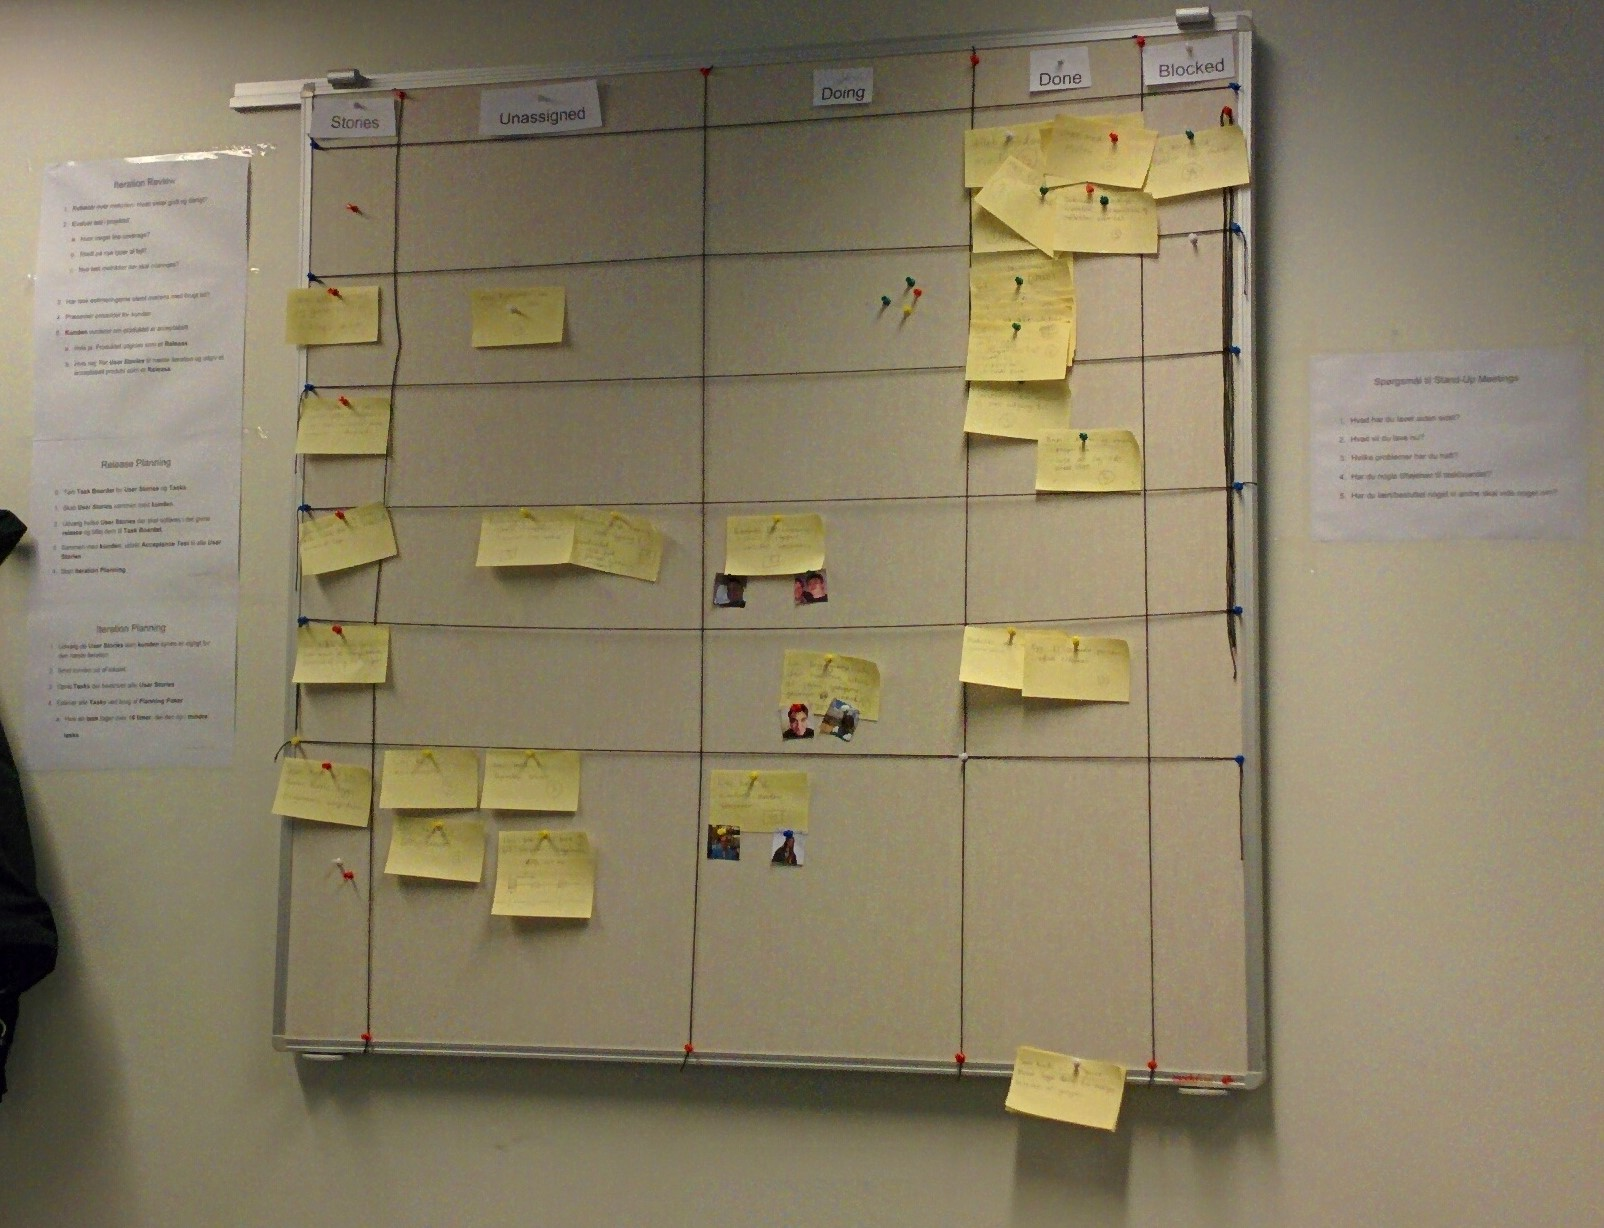
\includegraphics[width=0.7\textwidth]{method/taskboard.jpg}
    \caption{A picture of our taskboard.}
    \label{fig:taskboard}
\end{figure}

The user story cards are made in collaboration with the customer during release planning.  A subset of all the stories will then be selected to be completed in the given iteration, and acceptance tests will be made for these stories. An acceptance test is a specific test that is conducted in order to determine whether the specification or contract is met. And example of a user story and corresponding acceptance test can be seen in \tabref{tab:user_story_acceptance_test_example}. The rest of the user stories and acceptance tests can be found in \appref{app:user_stories_and_acceptance_test}.

\begin{table}[!htbp]
    \centering
    \begin{tabular}{| m{0.45\textwidth} | m{0.45\textwidth} |}
        \hline
        \textbf{User Story} & \textbf{Acceptance Test} \\ \hline
        As a customer, I would like to get answers from questionnaires generated by me from participants & 
        \begin{itemize}[noitemsep,parsep=0pt,partopsep=0pt]
        \item When a customer can come up with a questionnaire, get it into the system without writing code, and have it answered by a participant.
        \item The questions must occur in sequence and it should only be possible to answer yes or no.
     \end{itemize} \\ \hline
    \end{tabular}
    \caption{Example of a user story and corresponding acceptance test from our first iteration.}
    \label{tab:user_story_acceptance_test_example}
\end{table}
\FloatBarrier

We have chosen attempt to follow the standard XP release plan concept by playing various roles from XP, because they are such a central aspect of the method. For this reason during the iteration review and planning meetings we assign each team member roles, such as customer, tester, developer, and user, which they must role-play. This role playing makes it easier for us, as a team, to prioritize user story cards because one team member only has to consider one mindset during these meetings. This approach might be challenging because it can be difficult to apply a different mindset than what we are used to. This means that one team member is assigned to act as the customer during the entire review/planning meeting. As mentioned previously, another central aspect of the development is to have a representative for the customer on-site. However, this project is a student project without a paying customer or user, and we have therefore dediced to include role-play to compensate for this. 
\\\\
This role-playing, at least from a customer perspective, is guided by a vision of the system as developed using methods from Essense, see \ref{cha:vision}.

\todo[inline]{Måske tilføje argument omkring innovation og at der ikke behøver at være en dedikeret customer - Måske tilføje noget med at role play så er baseret på et vision?}

\subsection{Knowledge Sharing}
\label{sub:knowledge_sharing}
Knowledge sharing is encouraged in XP by using different practices such as daily stand up meetings. Daily stand up meetings are short meetings where the group members share thoughts about their current progress, hardships, and successes. This allows for brief insight in the collective progress of the group. Another core practice is pair programming, where two programmers sit at the same PC and develop together. Even though the main purpose of pair programming is to increase code quality it also allows for knowledge sharing between the programmers. 
\\\\ 
For us, knowledge sharing is important, since all members of the group should have insight in the product and the written report. We have therefore chosen to use daily stand ups and pair programming / writing in our process. We expect that these practices will increase the feeling of collective ownership over the project, provide a steady pace during development, and increase the quality of the project. 

\subsection{Test Driven Development}
\label{sub:test_driven_development}
Extreme Programming emphasizes that test driven development is the only development method that ensures that the developed program works as intended and is tested without using any shortcuts (i.e. the developer writes test-to-pass instead of test-to-fail). In previous semesters we have been lacking a structured approach to testing and evaluating during the development. Tests and evaluations have therefore previously been executed in ad-hoc fashions, which has not been as useful for us as we could have hoped. In an agile development method, we hope that a test-driven approach will help us solve this problem and achieve a more structured approach to enforce testing and increase code quality.
\\\\
We have not been working with XP or general acceptance testing in previous semester projects, and we therefore cannot judge the quality of the acceptance tests we will create for our user stories.

\subsection{Documentation}
A major part of the XP method is to maintain focus on development and not documentation, and it is only considered in XP if it gives the customer value. This is a very counter-intuitive approach in a student setting, because we have a requirement for the project that states necessary documentation of learning and reflection. 
\\\\
Due to the fact that XP does not not have any built in practices or techniques to produce a technical student report during development, we have to adapt our development method to include the production of such a report. We attempt to do this by having a miscellaneous user story on the task board which is allowed to contain tasks regarding documentation and setup for development environment etc. However since XP drives by commitment, this miscellaneous user story will, based on experience from previous semesters, be filled with tasks that is less interesting to perform. For that reason we also intend to have report iterations that should deplenish these types of tasks, where these tasks are the only ones allowed to work on.

\subsection{Continuous Integration}
\label{sub:continuous_integration}

Continuous Integration (CI) is the practice of frequently merging all the individual works in development from separate developers, ideally several times per day. This ensures that the system is always in a stable state, such that only small changes have to be taken care of in the case that something breaks, instead of having to roll back days, weeks or even months of work. CI is especially useful in test driven development, because the tests can simply be executed when people are integrating their work, which easily ensures the quality of the product. CI systems can also be configured to run nightly builds, which ensures that the system does not break due to outside factors, and also provides the ability to run tests that take long time to run.
\\\\
We think that a stable system is a very important part of our project, and we will therefore make a CI server. This server will automatically be notified about changes when we push our work to our version control system, and also run nightly builds. We hope that this will make it easier for us to spot errors during the development, such that the system is at a stable state during the entire development period. 
%!TEX root = ../../super_main.tex

\section{Essence}
\label{sec:essence}

\todo{Overvej at nævne flere Essence ting her hvis vi bruger dem}




% === ANALYSIS === %
%!TEX root = ../../super_main.tex

\chapter{Problem Analysis}
\label{cha:problem_analysis}

We need to conduct some initial analysis in order to be able introduce and concretize the problem. This chapter includes an overview of existing solutions that we have discovered, and we describe general strategies that can be done when developing for mobile platforms. Hereafter, we describe what the possible contexts that can be derived from sensors, and different approaches to human activity recognition. The chapter ends with a description of the personal data legislation and the problem definition.

%!TEX root = ../../super_main.tex

\section{Existing Solutions}
\label{sec:existing_solutions}
Some solutions that uses data gathering in the world of mental health have been investigated. It seems that a lot of software have been designed to improve mental health using mobile sensor data gathering. We will discuss two solutions that both monitor subjects using smartphone sensors and have these subjects fill out surveys. We here refer to subjects as both participants of a data gathering systems and individuals involved in medical research.

\subsection{Ilumivu mEMA}
\label{sub:ilumivu_mema}
There exists a concept called Ecological Momentary Assessment (EMA) \parencite{shiffman2008ecological} in mental health care, which is a way of making assessments of patients in the ecosystem where they normally exist. In traditional medical practice the patient is acquainted with a doctor, where long term treatment is periodical appointments with a doctor. This particular pattern has disadvantages in psychological treatments where the treatment does not happen in the environment where the patient lives, but it happens in a doctors or psychiatrist office. EMA is a way of gathering information from patient and possibly providing some sort of treatment or intervention in real-time. This type of system works particularly well using mobile technologies.
\\\\
Ilumivu have developed a Mobile EMA (mEMA) application \parencite{lumivu}. This application provides researchers and companies with a platform for real-time data gathering from test subjects going about their daily lives. The functionality in the purchasable core package of mEMA includes questionnaires and creation of these. It is also possible for the customers to add certain opt-ins that can provide more context for the answers of the questionnaires, such as mobile sensors, wearable sensors, and in-home sensors. The system is centered around the patient, and is generally meant for research purposes.

\subsection{AndWellness}
\label{sub:andwellness}

% AndWellness
AndWellness \parencite{hicks2010andwellness}, is another sensor monitoring/questionnaire focused system for Android phones. AndWellness have some interesting points on architecture and principles to do this type of monitoring. This system has a concept of a campaign which is the definition of studies, meaning it is the configuration of how sensor data is gathered and surveys are filled on the subjects smartphones. These configurations include how sensors should be monitored in terms of frequency and duration. It is also possible to configure how subjects are notified. AndWellness allows configuration of different triggers for questionnaires. These triggers can be set to be both temporal but also sensor activity based, meaning that both time and the activity and movement of the user can trigger sensor monitoring and notifications with surveys. This means that the customers using AndWellnes is able to customize their study in great detail, which is preferable as the purpose of the gathered data may vary. Lastly an idea to note is that this system has a concept of expiring surveys, meaning that the customer can configure for how long the subject may prolong a survey with a time window where the survey exists. These time windows allows customers to disallow meta cognition, the process of reflecting about ones thoughts. Some mental health studies does not want meta cognitions, i.e. no reflection after some activity, while other studies include meta cognitions as an important factor. 
\\\\
The AndWellness system allows for full transparency, meaning that subjects have full access to the data they are gathering for the customers, to increase trustworthiness. Lastly AndWellness does not support raw sensor output logging, they derive some soft sensors which they call Location- and Activity trace sensors. This is a potential flaw, because the data used to derive output cannot be converted back to raw sensor output and a mental health study might need data which is not included in the outputs of these predefined soft sensors.
\\\\
mEMA and AndWellness both monitor and report sensor readings in real time, meaning that they are highly connectivity dependent. It is not clear what these systems do in cases where there is no network access, but they stream the data directly to a server in almost real time when the phone is connected to a network. This type of network communication is counter intuitive with general practices on battery and network management. Furthermore these systems do not yet include a larger ecosystem of devices. For instance, these systems do not consider wearable technologies such as smartwatches and smartbands. This excludes some potential sensor information which is usually not present in smartphones.

% + Principle of campaign. %
% + Sensor monitoring have configurable resolutions (our terms: measurement frequency, sample duration, sample frequency).
% + Have different triggers, temporal, contextual (sensor). 
% + Triggers can both be camgaign-wise and participant specific.
% + Prompts for surveys.
% + Surveys expire, configured by admins of campaign (answering window).
% + Users have full transparency of the data gathered
% - Pure realtime, battery drain, very network dependent.
% - Pure smartphone, no wearable technology.
% - Only two derived (software sensors), Location and Activity tracing.
%     - No raw sensor output
% Purple Robot
\subsection{Purple Robot}
\label{sub:purple_robot}
Purple Robot \parencite{purple_robot} is an Android application originally developed to allow for easier or better integration for the PhoneGap and Apache Cordova applications with native functionality on the Android platform. The application allows other non-native applications to trigger status-bar notifications, application widgets, and full native dialogs. The application also allows other applications to access all the sensors on a device with an uniform interface. 
The communication for triggering and reading of the sensors is done using a locally running HTTP server that the Purple Robot application runs. This means that the Purple Robot application actually does not provide a lot of functionality for a user on its own, but allows other applications to have easy access to the integrated native functionality.
% This framework could be used to create what we are striving for?
This framework could be used to create access to native functionality, i.e. the sensors of an Android device, without having to build and maintain an Android application. Users could be asked to download and install Purple Robot instead. The framework supports delayed and encrypted uploads of collected data. 

\subsection{Sensor Data}
\label{sub:sensor_data}
Like Purple Robot, Sensor Data is an iPhone application for gathering unlabeled data. The application can gather data from all the sensors that are available in iPhone devices, which is then made available through a web API. It is possible to store the sensor data in two different ways when using Sensor Data: Capture Mode and Streaming Mode. When using Capture Mode the data is stored directly into the flash memory of the iPhone, while using Streaming Mode will transfer the data to another computer. The data is recorded and stored as comma separated values for easy integration into data analysis software.
\\\\
%Trust in third part
It might already be a challenge for us to gain the trust of participants. We are handling sensitive information about their everyday activities and life. Installing a third part application to handle this information could become a potential trust issue. We have installed the Purple Robot application on our devices and found the graphical user interface in the application to be unstable with seemingly random breakdowns. We have found this application and concept interesting, but we have found the application too unstable to be practical.   


%!TEX root = ../../super_main.tex

\section{General Strategies}
\label{sec:general_strategies}
To understand the mobile platform better we investigate some of the general strategies that are considered to be good practices for the mobile platform. A common strategy is to avoid sloppy handling of network communication, since this is a common source of battery drain in both the Android development community \parencite{android_network_scheduling} and Apple development community \parencite{iphone_network_scheduling}. Gathering training data with the purpose of training an AI model does not require the training data to be delivered in real time, unless the model itself is actually required to be trained and completed within a given temporal frame, which provides the possibility of respecting the battery drain of transferring data. 
\\\\
A common method to reduce network communication is to compress the data being sent \parencite{har_wearables}\parencite{android_network_scheduling}. This reduces the amount of data that has to be transferred, i.e. the amount of packets, and the awake-time of the network module. Another possibility is to communicate in bulks, which means that instead of sending many small packages with breaks in between, these can be collected into bigger packets \parencite{android_network_scheduling}. This will reduce the overhead of activating the communication module. The bulk transfer solution requires the data to be aggregated over time, which requires some sort of intermediate storage. This can be achieved by storing the data in memory for small data packets or persistently on a device for larger packets. Storing the data persistently on the device will also remove the risk of losing the data due to device crashes, and the data therefore becomes less volatile. Another side-effect of storing data, either persistently or in memory, is the possibility collecting data when there is no available connection or only a connection with a high power consumption, e.g. cellular network, and then sending it when a desired connection becomes available. Other typical techniques for reducing power consumption include \parencite{android_network_scheduling}:

\begin{itemize}
	\setlength\itemsep{-0.3em}
    \item Pre-fetch network data
    \item Network scheduling services
    \vspace{-0.8em}
    \begin{itemize}
    	\setlength\itemsep{-0.3em}
    	\item Use the network when other uses it
        \item Bundle outgoing data (cache outgoing data)
    \end{itemize}
    \vspace{-0.6em}
    \item Reduce number of connections
\end{itemize}

The idea of aggregating and minimizing network communication in a sensor network to save power is not a novel one \parencite{korteweg2007data} \parencite{mhatre2004design}, but this practice seems to be violated in the existing solutions. A battery consumption aware application which collects data, but does not synchronize it with a server in real time, could offer substantial battery consumption improvements to existing solutions.

%!TEX root = ../../super_main.tex

\section{Deriving the Context from Sensors}
\label{sec:deriving_the_context_from_sensors}

To realize the vision (\secref{sec:vision})\todo{forward reference}, the devices we are going to develop a solution for must be able to provide data that can be used to derive something about context in which the participants exist. This section describes how different sensors may contribute to describing the reality around participants, in as much detail as possible. Note that there might be differences in the quality of the sensors, since not all devises are using the exact same sensor.
% We only consider sensors that are commonly found in mobile devices and smart wearables compatible with Android. 

\subsection{Availability of Sensors}
To discover which sensors are commonly available and how different type of devices can contribute, the specifications of some popular smartphones and wearables have been analyzed. \tabref{tab:sensors_in_devices} gives an overview of which sensors are available from each of these devices. 

%!TEX root = ../../super_main.tex

\begin{sidewaystable}
\centering
\begin{tabular}{|l|c|c|c|c|c|c|c|c|}
\hline
 & Nexus 5 & \begin{tabular}[c]{@{}c@{}}OnePlus \\ One\end{tabular} & \begin{tabular}[c]{@{}c@{}}Samsung \\ Galaxy S3\end{tabular} & \begin{tabular}[c]{@{}c@{}}Samsung \\ Gear S\end{tabular} & \begin{tabular}[c]{@{}c@{}}Microsoft \\ Band 2\end{tabular} & Moto 360 & \begin{tabular}[c]{@{}c@{}}LG Watch \\ Urbane LTE\end{tabular} & \begin{tabular}[c]{@{}c@{}}Huawei\\ Watch\end{tabular} \\ \hline
Accelerometer & \checkmark & \checkmark & \checkmark & \checkmark & \checkmark & \checkmark & \checkmark & \checkmark \\ \hline
\begin{tabular}[c]{@{}l@{}}Ambient\\ Light Sensor\end{tabular} & \checkmark & \checkmark &  & \checkmark & \checkmark &  &  &  \\ \hline
Barometer & \checkmark &  & \checkmark & \checkmark & \checkmark &  & \checkmark & \checkmark \\ \hline
\begin{tabular}[c]{@{}l@{}}Cellular\\ Networking\end{tabular} & \checkmark & \checkmark & \checkmark &  &  &  & \checkmark &  \\ \hline
Compass (Magnetometer) & \checkmark & \checkmark & \checkmark & \checkmark &  & \checkmark & \checkmark &  \\ \hline
\begin{tabular}[c]{@{}l@{}}Galvanic Skin\\ Response Sensor\end{tabular} &  &  &  &  & \checkmark &  &  &  \\ \hline
GPS & \checkmark & \checkmark & \checkmark & \checkmark & \checkmark &  &  &  \\ \hline
Gyroscope & \checkmark & \checkmark & \checkmark & \checkmark & \checkmark & \checkmark &  & \checkmark \\ \hline
\begin{tabular}[c]{@{}l@{}}Optical Heart\\ Rate Sensor\end{tabular} &  &  &  & \checkmark & \checkmark & \checkmark & \checkmark & \checkmark \\ \hline
Proximity Sensor & \checkmark & \checkmark & \checkmark & \checkmark &  &  & \checkmark &  \\ \hline
\begin{tabular}[c]{@{}l@{}}Skin Temperature\\ Sensor\end{tabular} &  &  &  &  & \checkmark &  &  &  \\ \hline
UV Sensor &  &  &  & \checkmark & \checkmark &  &  &  \\ \hline
Wi-Fi & \checkmark & \checkmark & \checkmark & \checkmark &  &  & \checkmark & \checkmark \\ \hline
\end{tabular}
\caption{Available sensors in each mobile device that we have considered.}
\label{tab:sensors_in_devices}
\end{sidewaystable}
\FloatBarrier

\subsection{Continuous Sensors}
A single or few reading form this type of sensor does not give much value to describe a context. However, a continuous stream of readings describes change over time of the context, thus grating value. These sensors are often noisy i.e. the read vary a bit from the expected value even though the device is laying perfectly still.

\begin{description}
	\item[Accelerometer] measures the acceleration of the device in three dimensions, which is also often together with the gyroscope sensor. The accelerometer is able to provide measurements that can describe the motion of the wearer or user along the three physical axes, typically measured in $m/s^2$.
	\item[Gyroscope] measures the speed of rotation of the device in space. The gyroscope will provide an idea of the orientation of the device relative to Earth's gravitational pull. The rotation of the gyroscope is measured on all three axises as rotation velocity in $rad/s$.
	\item[Compass] (also known as magnetometer) is able determine the orientation of the device relative to the Earth's magnetic field. This sensor can, in combination with the accelerometer be used to provide readings like that of a compass. The magnetometer measures the magnetic influence on all threes axises in $\mu T$.
	\item[Barometer] approximates the air pressure, in $hPa$ or $mbar$, around the device. The readings from a barometer can be used to estimate the altitude of the device.
    \item[Optical Heart Rate Sensor] estimates the heart rate, using a light source and a light sensitive sensor. Heart rates are measured in Beats per Minute (BPM). It can be used to detected elevated heart rate levels for instance caused by exercising or heightened levels of stress. Heart rate monitoring can also be used estimate the quality of ones sleep \parencite{guardian_fitness_tracker_rem_sleep}. 
    \item[Skin Temperature Sensor] measures the temperature of skin that touches the device, given in some type of degrees, usually Celcius. This can possibly indicate environmental effects on the body temperature, exercising, fever, etc.
    \item[Galvanic Skin Response Sensor] (GSR) measures the conductivity of the surface against the device. This can indicate whether or not a person is sweating, or more generally the moisture level on a surface. The GSR sensor is commonly used to infer whether a wearable device is being worn at the moment, and its output is measured in ohm ($\Omega$).
\end{description}

\subsection{Reactive Sensors}
Sensors described in this section are reactive meaning that they output measurements when an event from the environment triggers them. The events are typically used to handle some change in the environment rather than measuring the context.

\begin{description}
    \item[Proximity Sensor] can estimate how close the device is to the nearest object facing the sensor by using an infrared beam. This estimation has higher accuracy in lower distances. The distance is measured in $cm$. Some devices, however, does not measure the distance directly but return binary values that represent ``near'' or ``far'' instead of an actual distance, the output is still outputted as either zero or five centimeter. This sensor is commonly used to turn of the display when the device is placed in the pocket or is held against the ear.
    \item[Ambient Light Sensor] makes it possible to measure the illumination surrounding the device in $lx$. This is commonly used to regulate the background light of the device's screen.
    \item[Ultraviolet Sensor] (UV) measures the UV radiation hitting the device. This is useful for estimating whether a person is inside or outside. It can also be used to estimate whether a person has spent too much time outside, and thereby in risk of sunburns or skin cancer, by accumulating readings of UV radiation of an entire day. The output of the UV sensor in the Microsoft Band 2 is given by an enum with the values: none, low, medium, high, and veryhigh, which corresponds to different levels of UV indexes. 
\end{description}

\subsection{On-Demand Sensors}
On-demand sensors are sensors that have do not provide a stream of information but have to be requested whenever a measurement is needed. Measurements from this type of sensors are typically more expensive in terms of battery consumption and computation. An on demand reading can only be given asynchronously as the device would first have to contact multiple information providers such as cell towers and GPS satellites and over time reach a sufficiently accurate reading. To improve efficiency the latest readings are, for example in Android, cached, which allows for quick access the most recent result.

\begin{description}
    \item[Wi-Fi] in mobile devices can be used for more than just pure data communication with the local network and the Internet. Different information about access points and the signal to these access points can for instance be used to approximate indoor location. Features of Wi-Fi networks could be reachable access point names, their communication standards, and signal strength. 
    \item[Global Positioning System] (GPS) approximates the latitude and longitude of the device based on satellite triangulation. Most modern mobile devices use Assisted GPS (A-GPS), meaning that the GPS is assisted by the cellular network. The rough positioning is based on the cellular network and the accurate position is triangulated using GPS satellites. Some systems can also provide estimated information about speed and bearing of the device.
    \item[Cellular Networking] can, similarly to Wi-Fi be used for more than pure communication as data from different mobile towers and the signal strength to these towers can be useful besides communication. Potentially interesting features could be country code, network code, cell identity (mast identity), cell tower technology type, and signal strength.
\end{description}

We have briefly looked at the availability of various sensors in different smart devices, and it generally seems like most devices have many of the same sensors. In relation to our project this means that we can choose to develop a solution for either iPhone, Android or Windows Phone and their related wearables without limiting the available sensors. A context can at the same time be measured by multiple sensory devices in order to increase the accuracy of the data, which suggests combining outputs from multiple of the examined sensory devices. 
\\\\
Some of the sensors furthermore describe overlapping parts of the context, and we have therefore initially chosen not to include cellular networking as a data source directly. There is a lot of data to be found from this sensor, but the features and the layout of the data differs depending on which cellular technology the cell tower supports, which makes it slightly difficult to implement. The location of the user is already indirectly available through A-GPS and cellular positioning, and we have therefore decided not include this data source initially. 
\\\\
There are also other available sensors that we have not yet taken a look at in order to describe contexts, such as bluetooth, screen wake time, use of apps, etc. We will not exclude the possibility of using these at some point during the development, but we think the sensors from \tabref{tab:sensors_in_devices} describe an initial sensor context that we can use in order to build a base product. 

%!TEX root = ../../super_main.tex

\section{Human Activity Recognition}
\label{sec:human_activity_recognition}

Since we want to provide data for reality mining we must consider how we want to approach human activity recognition. There are at least two overall different approaches to this namely participatory and opportunistic sensing \parencite{opp_or_par} \parencite{har_wearables}. Participatory sensing requires that participants actively participates in the data collection by own initiative, directly entering data, or by otherwise reacting to requests for input. Opportunistic sensing requires less to none involvement from the participant but it does require more passive monitoring of the context of the participant even when the system is not actively gathering data in order to sense if the participants context matches triggering conditions for a campaign. A platform that gathers data for reality mining would have to actively monitor or somehow be aware of when participants are physically located near an area of interest. A configuration of a campaign (it is analogue with the term application query of \parencite{opp_or_par}) could for instance require that data should be gathered when the participant is drinking coffee i.e. they are near a coffee shop. This constant monitoring of the participants context, in order to enable triggers, might though present its own privacy intrusion problems. This monitoring could however be performed strictly locally on the mobile device of the participants and wearables and the participants privacy could thus be somewhat preserved.
\\\\
The two approaches can be combined where opportunistic sensing could then provide context in the shape of features used to learn classes provided from participatory sensing where participants are included to provide the target classes, i.e. labels, in a training data set. Opportunistic sensing could also provide triggers for when participants should be involved in the process. Allowing customers to configure a campaign could then allow customer of the system to specify to which degree they want participant involvement, i.e. participatory sensing, and when and how they want it, i.e. opportunistic sensing.
\\\\
The amount of different classes or labels one could infer directly from the sensor data is somewhat limited and would not allow many possible classes which captures human behavior or state. One could attempt to setup artificial rules and determine the labels in the data based on these rules, these rules would however likely be based on assumptions about the data, unless some other ground truth is known, and it would be difficult to infer many possibly interesting human behavior or state classes for a desired artificial intelligence (AI) model such as for instance stress levels or happiness. One might however with a given algorithm or another machine intelligence model be able to recognize patterns in the data to infer classes, this could for instance be if the person is dancing or not, e.g. by detecting rhythmic movement.    
\\\\
One way to involve participants could be questionnaires with one or more questions. The answers could then determine the labels of the data, or it could be seen as features. The validity of this participant generated data would depend on the truthfulness and perception of the participants which could be a source of error. The validity of the data could however be evaluated and filtered by customers outside the data collection system. Data from external sensors or other certain combinations of values from the collected set of features for each sample, i.e. the participants context, might be helpful in determining the truthfulness of answers provided by participants.
\\\\
We will need to support some kind of participant involvement in order to be able to gather labels for the participants context. The success of the system thus depends on how willing participants are to participate, first by actually installing the data gathering application and secondly how actively participants are willing to participate and provide labels for the gathered contexts with respect to the campaigns specified by customers. It is thus up to the customers to design campaigns the participants are willing to participate in. The success of the system thus depends on the ability of the customers, given that the system works as intended.


%!TEX root = ../../super_main.tex

\section{Personal Data}
\label{sec:personal_data}

To realize the vision of our system (\secref{sec:vision}), the platform will have to collect various measurements from sensors in ubiquitous devices alongside some feedback from the participants using the platform. The collected data can resolve in a description of the individuals using the system, meaning that incorrect handling of this data could resolve in violating the users' privacy. For this reason we will have to consider how the system should respect privacy, both in terms of legislation and ethical considerations.

%!TEX root = ../../super_main.tex

\subsection{Legislation}
\label{sub:legislation}

With the increasing use of mobile devices in a society where everything is being digitized, the gathering of data also increases. This digitization means that all sorts of data are being collected about the average citizen. This data collection happens in both the public sector and private sectors. The government, as part of the public sector, gathers information regarding health and taxing, while companies such as Facebook and Google gather personal data regarding the users behavior while using their applications. With the increasing amount of data being gathered, coming from personal devices such as smartphones and wearables, it is important to consider the legislative requirements related to storing personal data about people.
\\\\
Personal data is defined as information that allows for the identification of a single individual, either directly or indirectly. Directly referring to using unique identifiers such as CPR number, while indirectly could be done by tracking a person's movements and using this to identify the individual. The Danish laws about protecting personal data classifies personal data into different categories: Normal data and sensitive data. Sensitive data is defined as revealing racial or ethnic origin, political opinions, religious or philosophical beliefs, trade-union membership, and data concerning health or sex life \parencite{datatilsynet_stud1}, while normal data refers to everything else, such as name and address.  
\\\\
When located in Denmark one has to notify, and receive permission from, the Danish Data Protection Agency (DDPA), before being allowed to process (i.e. handle in any way) personal data. When processing data the reason has to be well-founded, and the processed data should be the minimum amount required in order to fulfill the purpose of the data collection. However, special rules apply for university students. The main difference for students is, that the DDPA does not have to be notified, and no permission is needed. The rest of the general laws regarding personal data still hold, such as encrypting data transfers, ensuring limited (password protected) access to the data, and having consent from the users. 
\\\\
The Danish law of protection of personal data is an implementation of the 95/46/EC directive of the European Parliament \parencite{eu_personal_data_law}. There has however been announced new legislation, General Data Protections Regulation (GDPR), in this area which will likely come into effect some time in 2018 \parencite{eu_data_law_changing}. The regulation contains a number of amendments to the previous directive, such as heavy financial penalties of up to 20 million euro or up to 4\% of annual worldwide turnover for groups of companies, whichever is greater, if they are to break the regulation. The danish legislation in the area has not been updated to meet these demands, and therefore we cannot know the exact implementation that we should follow. We have therefore chosen to follow the current Danish legislation for student projects, which as previously mentioned is less restrictive than the general legislation in the area. 


%!TEX root = ../../super_main.tex

\section{Ethical Considerations}
\label{sec:ethical_considerations}

With the increasing use of mobile devices in a society where everything is being digitized, the gathering of data also increases. This digitization means that all sorts of data are being collected about the average citizen. This data collection happens in both the public sector and private sectors. The government, as part of the public sector, gathers information regarding health and taxing, while companies such as Facebook and Google gathers personal data regarding the users behavior using their applications. With the increasing amount of data being gathered, coming from personal devices such as smart phones and wearables, considerations about how one store this type data becomes increasingly important. Professor of IT-ethics at Aalborg University deemed that personal data is one of the largest ethical dilemmas in the recent and upcoming years.

    % Med et voksende antal private og offentlige registre, hvortil flere og flere får adgang, vokser risikoen for tab af følsomme personoplysninger og misbrug af data. Det er det største etiske dilemma, vi går i møde i 2015.
\quotewithauthorandref{
	With a growing amount of private and public registers, where more and more people get access, the risk of loss and misuse of sensitive personal data increases. That is the biggest ethical dilemma we will face in 2015.
}{Thomas Ploug}{etik_dk_thomas_ploug}{true}

Experts deem that abuse of personal data is becoming an increasing risk. One must therefore tread carefully when this type of data is stored, transfered, and in general used. There exist legislation in Denmark that should ensure that these issues are being treated with care. However, because the value of personal data increases for malicious parties as well as non malicious parties, the devastation of it being accessible to the wrong people also increases. It should be in everyones interest to treat these personal data with care, since users have no direct control of how these data are access or who have access to it. Bill Schmarzo, chief technology officer for EMC Global Services, an influential cloud computing and -storage company, is particular concerned with unauthorized parties accessing personal data.

\quotewithauthorandref{
    But the bigger concerns are related to unsanctioned organizations using my data and inferences about my interests, passions, affiliations and associations for borderline uses about my political, religious, sexual, etc. preferences.
}{Bill Schmarzo}{forbes_bill_schmarzo}{false}

A safe and secure infrastructure should be established in systems operating with information that have potential to harm the people it was gathered from.

%!TEX root = ../../super_main.tex

\section{Problem Definition} 
\label{sec:problem_definition}
% Opsumer analyse
% Legal stuff, Encryption stuff, ethics stuff
There is, as described in \secref{sub:legislation}, different types of data with different privacy requirements. Some of these requirements apply to this project and the data we intend to collect. We must therefore take measures to accommodate these requirements. 
\\\\
% Campaign definition(s)
We borrow the terminology from AndWellness \parencite{hicks2010andwellness} and define a campaign to be all the configuration of triggers, sensor data collection, and label questionnaires necessary for a data collection from users    
\\\\
% Health care stuff requires real time - Impacts battery
Available sensor gathering applications and accompanying platforms generally have real time goals, health care systems often have intervention goals which requires data to be synchronized with a central node in near real time. 
\\\\
% Does not allow dynamic use of sensors from other mobile devices than smartphones
The existing solutions we have looked at does not incorporate more devices than smartphones which in general does not have all the health monitoring sensor of for instance a smart watch or a smart band, which opposed to a smartphones are worn close to the body. One could for instance imagine that data from these sensors to be interesting in various health related classification problems. 
\\\\
% Participatory sensing and training data
The context of monitored ubiquitous devices, i.e. gathered sensor data, does necessarily not provide much value without being coupled with a meaningful class label which could for instance be the mental state of a user through participatory sensing. The sensor data values, by them self, can only be used to train a model which predicts the behavior related to a subset of the sensors without the extra user provided labels.

% Hovedspørgsmål 
\subsection{Problem Statement}
\label{sub:problem_statement}

%Current health s

The following problem statement and supporting subquestions are based on the prior analysis.
\\\\
\textbf{What characterizes a participatory sensing system which collects machine intelligence training data from distributed ubiquitous devices and how could such a system be realized?}

% Underspørsmål
\begin{itemize}
    \item How can we facilitate ad-hoc sensor data collection of different ubiquitous devices, which might and might not be present at a given time?
    \item How can we acquire class labels, from users, for the sensor data context gathered from ubiquitous devices?  
    \item How can we allow customers to define a campaign for their users?
    \item How can we minimize battery consumption from data gathering on mobile devices by exploiting that we little real time requirements?
    \item How can we maintain legally required privacy of users and protect their sensitive personal data? 
\end{itemize}




% === VISION === %
%!TEX root = ../../super_main.tex

\chapter{Scope of Project}
\label{cha:scope_of_project}

We have investigated how we can approach the defined problem. This chapter explains the thought process we have been through when establishing our vision for our solution. This chapter will cover some scenarios that discuss different views for a possible solution as well as some vision representation that have been used in this creative part of the project. This chapter will finally describe the final vision of a solution we deem will answer the problem statement. 

%!TEX root = ../../super_main.tex
\section{Vision Scenarios}
\label{sec:vision_scenarios}

Essence, as mentioned in \secref{sub:essence_vision_scenarios}, suggests to utilize vision scenarios. We have come up with a list of opposing directions of development, which can be used to explore the different quadrants of a graph with two of the opposites as its axes. The purpose of this is to detail different directions the project could take and thereby learn more about the problem and possibly learn more about how it can be solved. We here present our candidates for possible opposing directions of development, that we could imagine pursuing for our project.

\begin{itemize}
	\setlength\itemsep{-0.2em}
    \item Disruptive/Non-disruptive - Should the system be based on passively collected sensor data or interactively prompt with questionnaires? % 1
    \item On demand/Continuous - Should the system be activated by participants or run continuously in the background? % 2
    \item Ease-of-use/Customizable - Should we require that customers must customize campaigns or should there be a predefined suite of campaigns % 3
    \item Assigned/Opt-in - Should campaigns be assigned automatically to participants using a participant profile or should participants actively choose campaigns? % 4
    \item Personal/Anonymous - Should the system require personal information about participants or not? % 5
    \item Open source/Strict ownership - Should the data gathered be open source or be strictly owned by the customer? %6
\end{itemize}

We will briefly elaborate our considerations about the various opposing questions, in order to explore our possible direction when moving forward with the project. 
\\\\
% Dem vi ikke har valgt
% 1
In regards to the \emph{Disruptive/Non-disruptive} bullet, we found it difficult to imagine the usefulness of a system that exclusively collects sensor data for classification problems. This means that at least some data, that is not read from sensors, should be collected, e.g. labels. The degree of disruptiveness could then perhaps be regulated by the campaign configuration. 
\\\\
% 2
Considering the \emph{On demand/Continuous} bullet, the system could allow participants to turn the system on and off easily, but we think that having the system running continuously once activated would increase the probability of completing campaigns. Actual data collection could depend on whether there is an active campaign on the participant's device. 
\\\\
% 5
For \emph{Personal/Anonymous}, we found that some demographic information would be interesting. Customers would likely be interested in whether the collected data represents the wide population or the specific group they are targeting for their data collection project. The degree of personal information required for a given campaign could perhaps then be defined in a campaign configuration. 
\\\\
% 6
Related to \emph{Open source/Strict ownership}, we found that it would be interesting if some of the collected information would be usable by multiple customers. This could prevent collection of redundant data to some degree, by allowing customers to specify an \emph{open source} campaign.
\\\\
We initially choose not to pursue the four abovementioned opposing directions of development, since we deem them to be unnecessary for an initial version of a solution for our problem. 
% Dem vi har valgt
% 3
We have instead chosen to include the \emph{Ease-of-use/Customizable} orientation question as the first axis, because we thought it would be interesting to explore different ways of allowing customers to configure what data they want, and how they want it, and because we think that both directions could add value. 
% 4
We have furthermore chosen the \emph{Assigned/Opt-in} orientation question for the second axis, because these directions would have a large impact on how a solution should be formed. We would have to store a lot of demographic data about participants, thereby possibly impacting privacy, if we want to assign and match campaigns. Both directions would impact how the interaction with participants should be designed, and which infrastructure we would need in order to support it.


%!TEX root = ../../super_main.tex

\section{Vision Representation}
\label{sec:vision_representation}

With the two orientation question, and hereby the four quadrants, decided upon, we have tried to to make two vision representations, namely the metaphor- and the proposition representation.

\subsection{Metaphor Representation}
\label{sub:metaphor_representation}

\begin{figure}[!htbp]
	\centering
	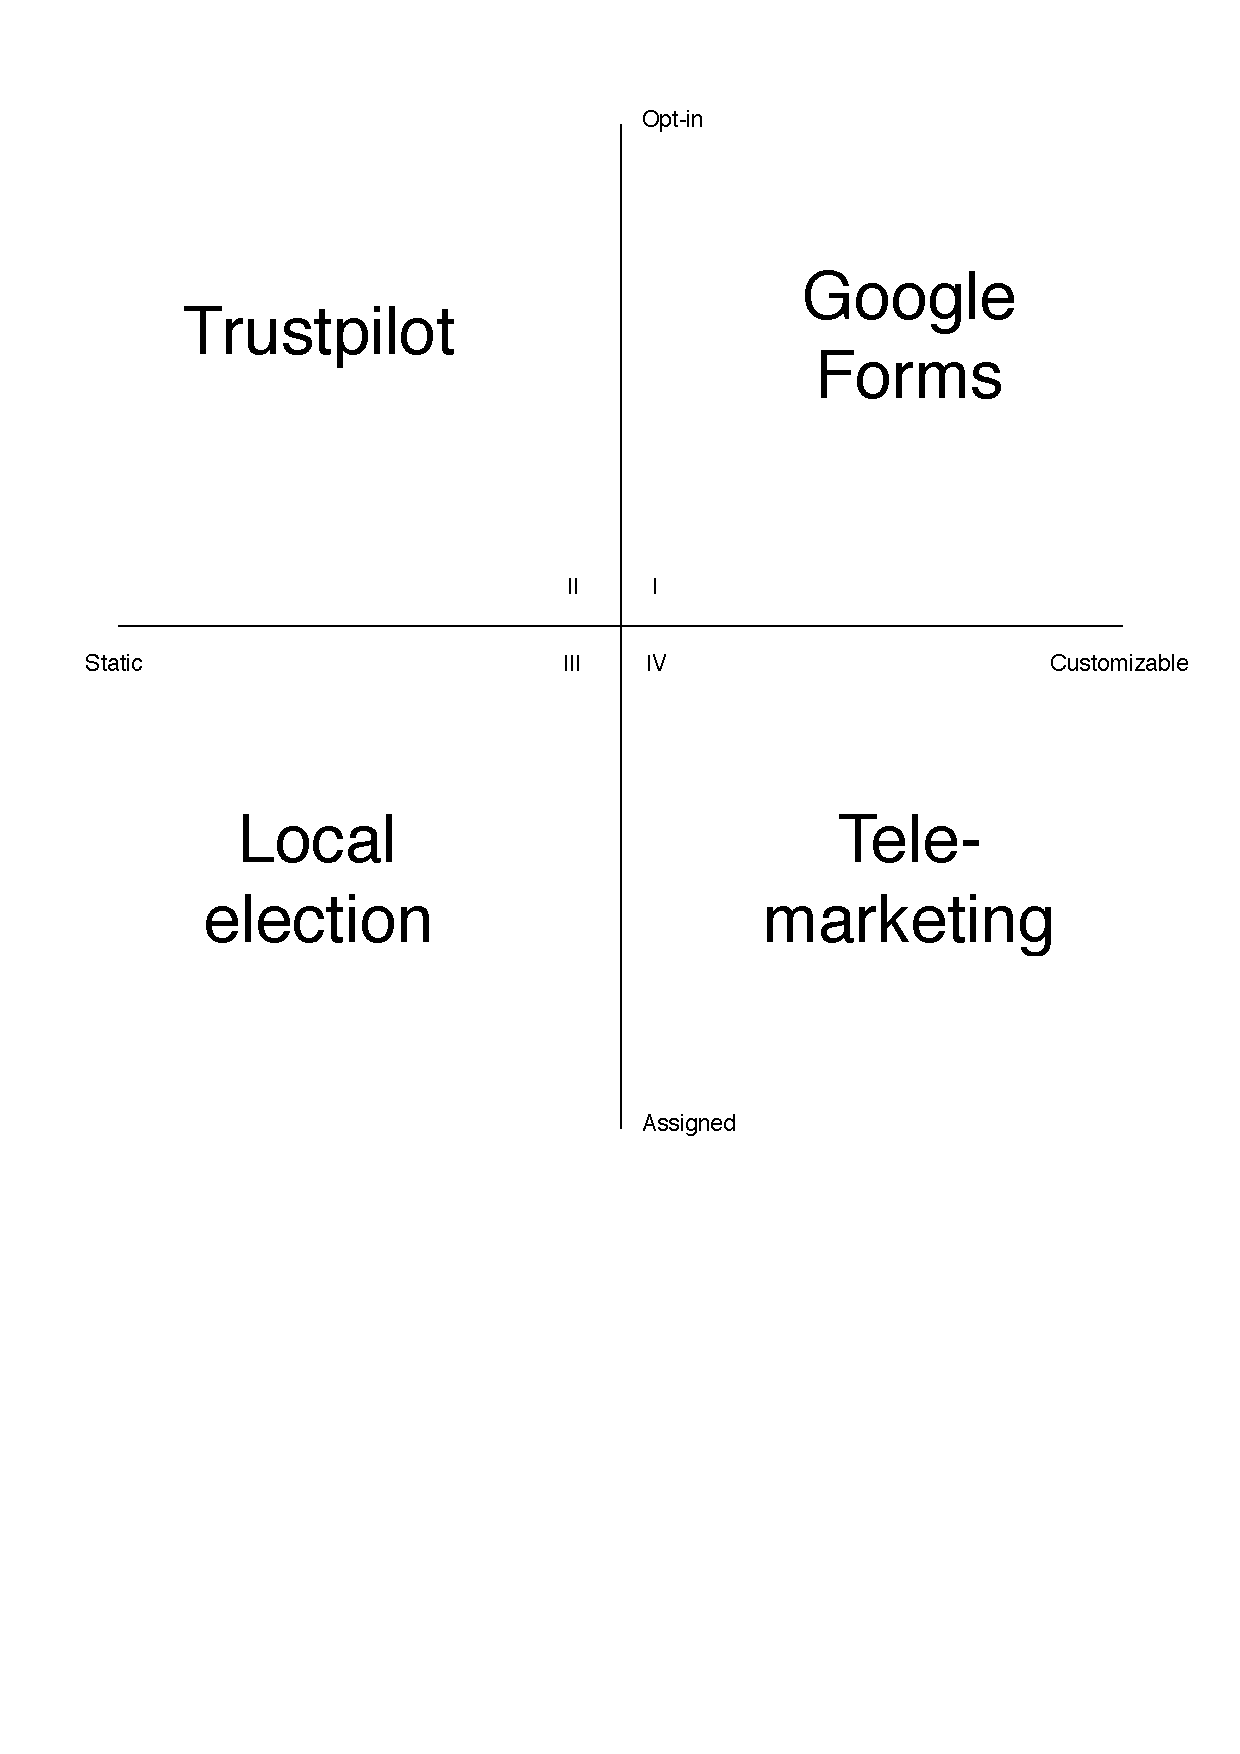
\includegraphics[width=0.8\textwidth]{graphic/problem_analysis/vision/metaphor.pdf}
	\caption{Four metaphors based upon the four quadrants.}
	\label{fig:metaphor}
\end{figure}
\FloatBarrier

\subsection{Proposition Representation}
\label{sub:proposition_representation}

\begin{figure}[!htbp]
	\centering
	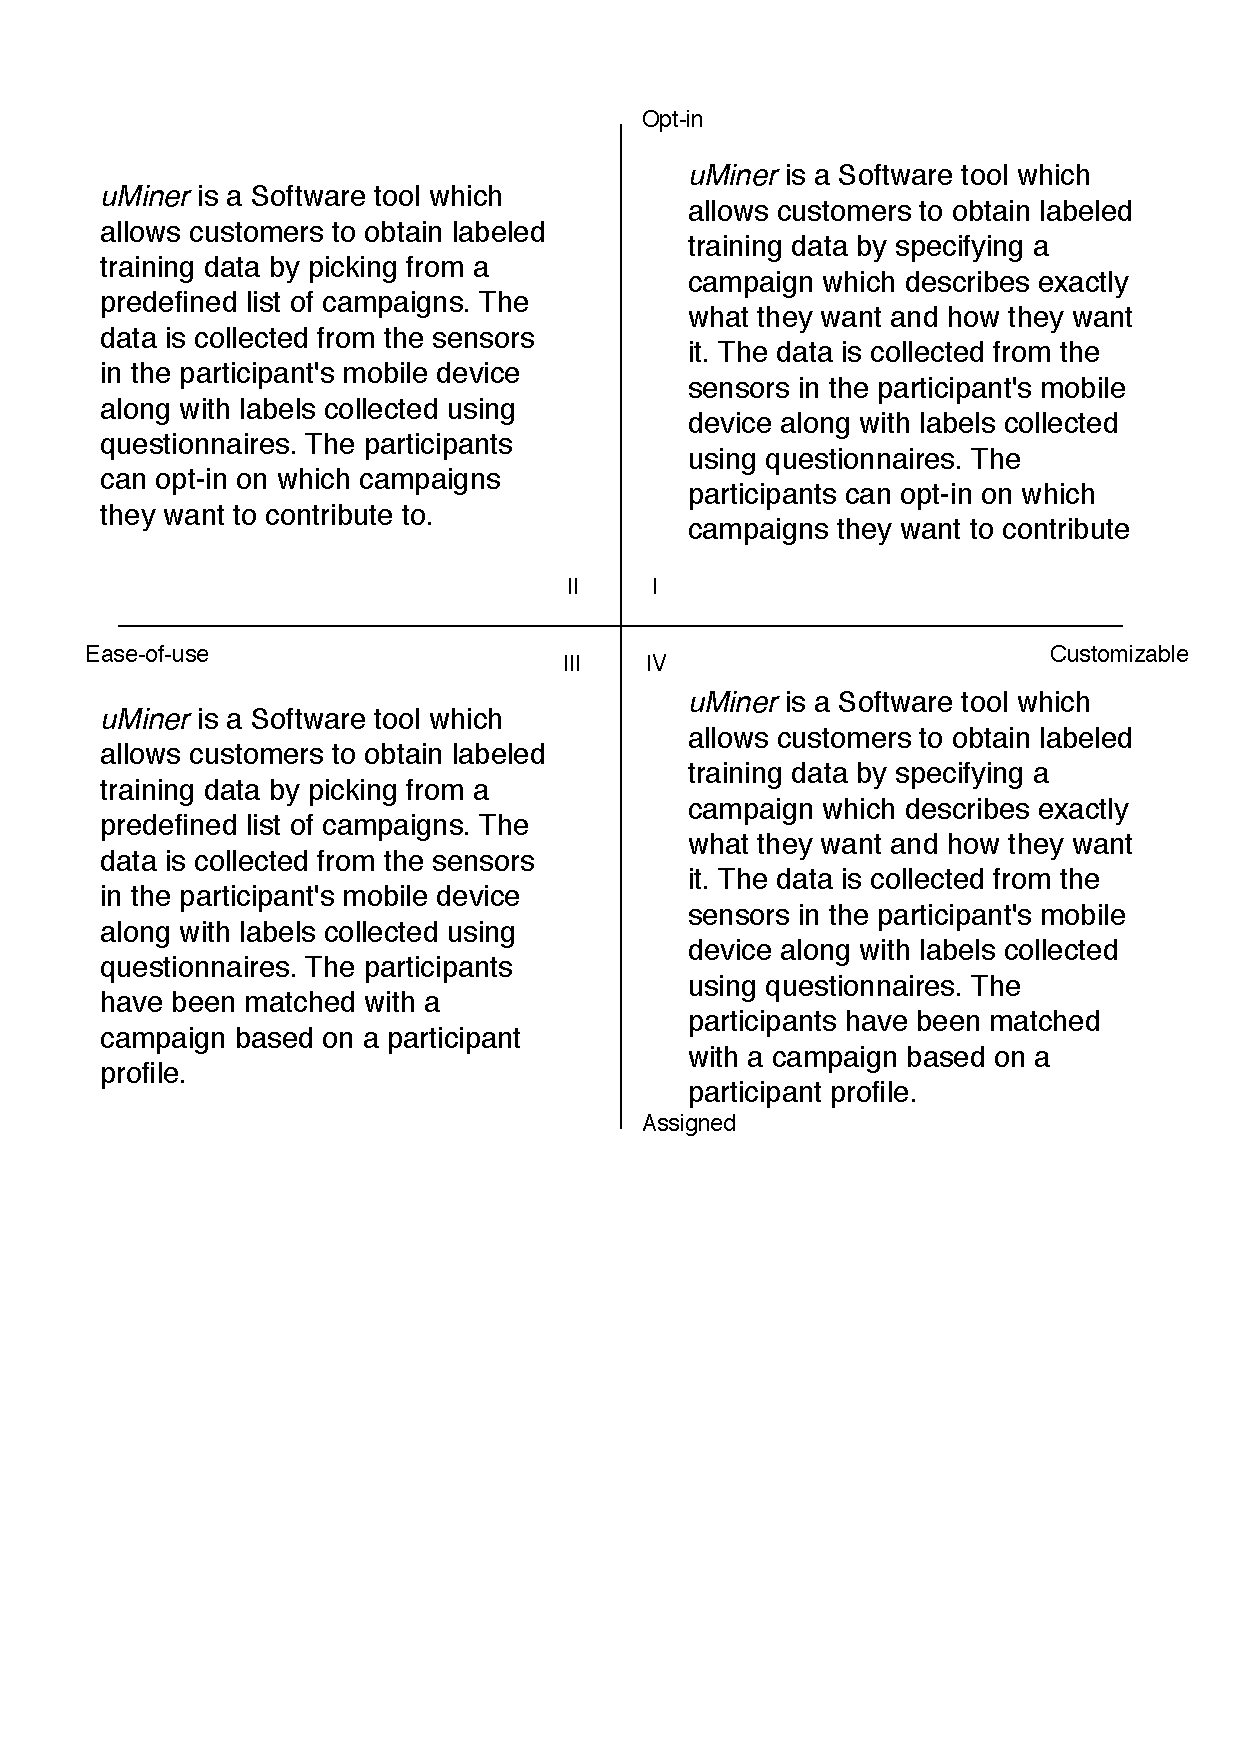
\includegraphics[width=0.8\textwidth]{graphic/problem_analysis/vision/propositions.pdf}
	\caption{Four propositions based upon the four quadrants.}
	\label{fig:proposition}
\end{figure}
\FloatBarrier

\todo[inline]{Figuren (\figref{fig:system_vision}) skal vist ikke lige stå her, måske i sektionen nedenunder}
\begin{figure}[!htbp]
    \centering
    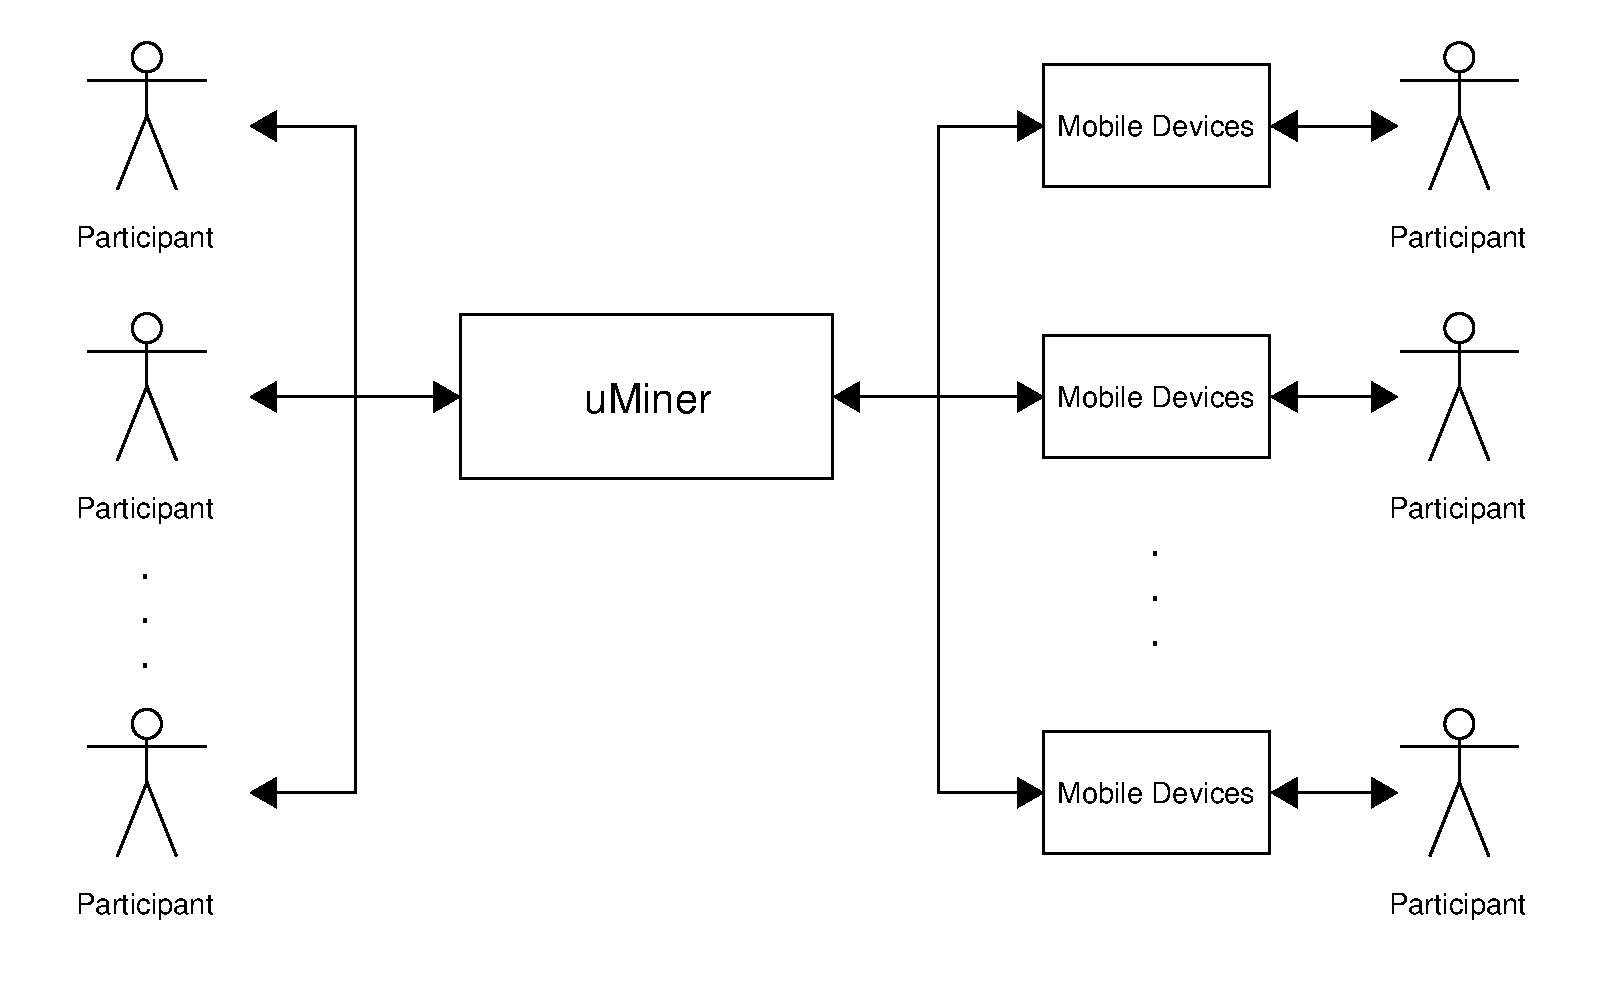
\includegraphics[width=\textwidth]{problem_analysis/vision/system_vision}
    \caption{The system vision.}
    \label{fig:system_vision}
\end{figure}
\FloatBarrier

%!TEX root = ../../super_main.tex
% Skal svare til Ivans: 2.6. Results from representation types and quadrants
% Her skal der tages en masse beslutninger baseret med vision scenarios etc. 
\section{Vision}
\label{sec:vision}
The vision for a solution for our problem is to develop a platform that allows for collection of data for reality mining. Different people who apply reality mining procedures often require different types of labeled training data. We would like to provide a platform that can gather snapshots, which will allow for human activity recognition. The campaigns should be configurable such that the gathered data can be useful for different purposes, for instance accumulating statistics or training a machine intelligence model. For this reason the platform should allow for configurable collection of snapshots. A customer should be able to to configure what type of information he wants in the snapshots, and how the labels of these should be derived, as well as define the demographic group that the campaigns should be available to. The vision for the platform is, that people, who are in need of context aware training data, can use our platform, instead of developing and distributing their own specialized applications to gather these type of data. The way we intend to concretize this, is to establish two different interfaces. One interface for customers, where they can specify campaigns, and another interface for participants that allows for gathering of data for reality mining. An illustration of this can be seen in \figref{fig:system_vision}. Here, customers specify the data the want, through the \emph{uMiner} system. This campaign specification is made available to all mobile devices, such that participants can join the campaign, and their smart devices will know how to ``mine'' the reality around the participants. 

\begin{figure}[!htbp]
    \centering
    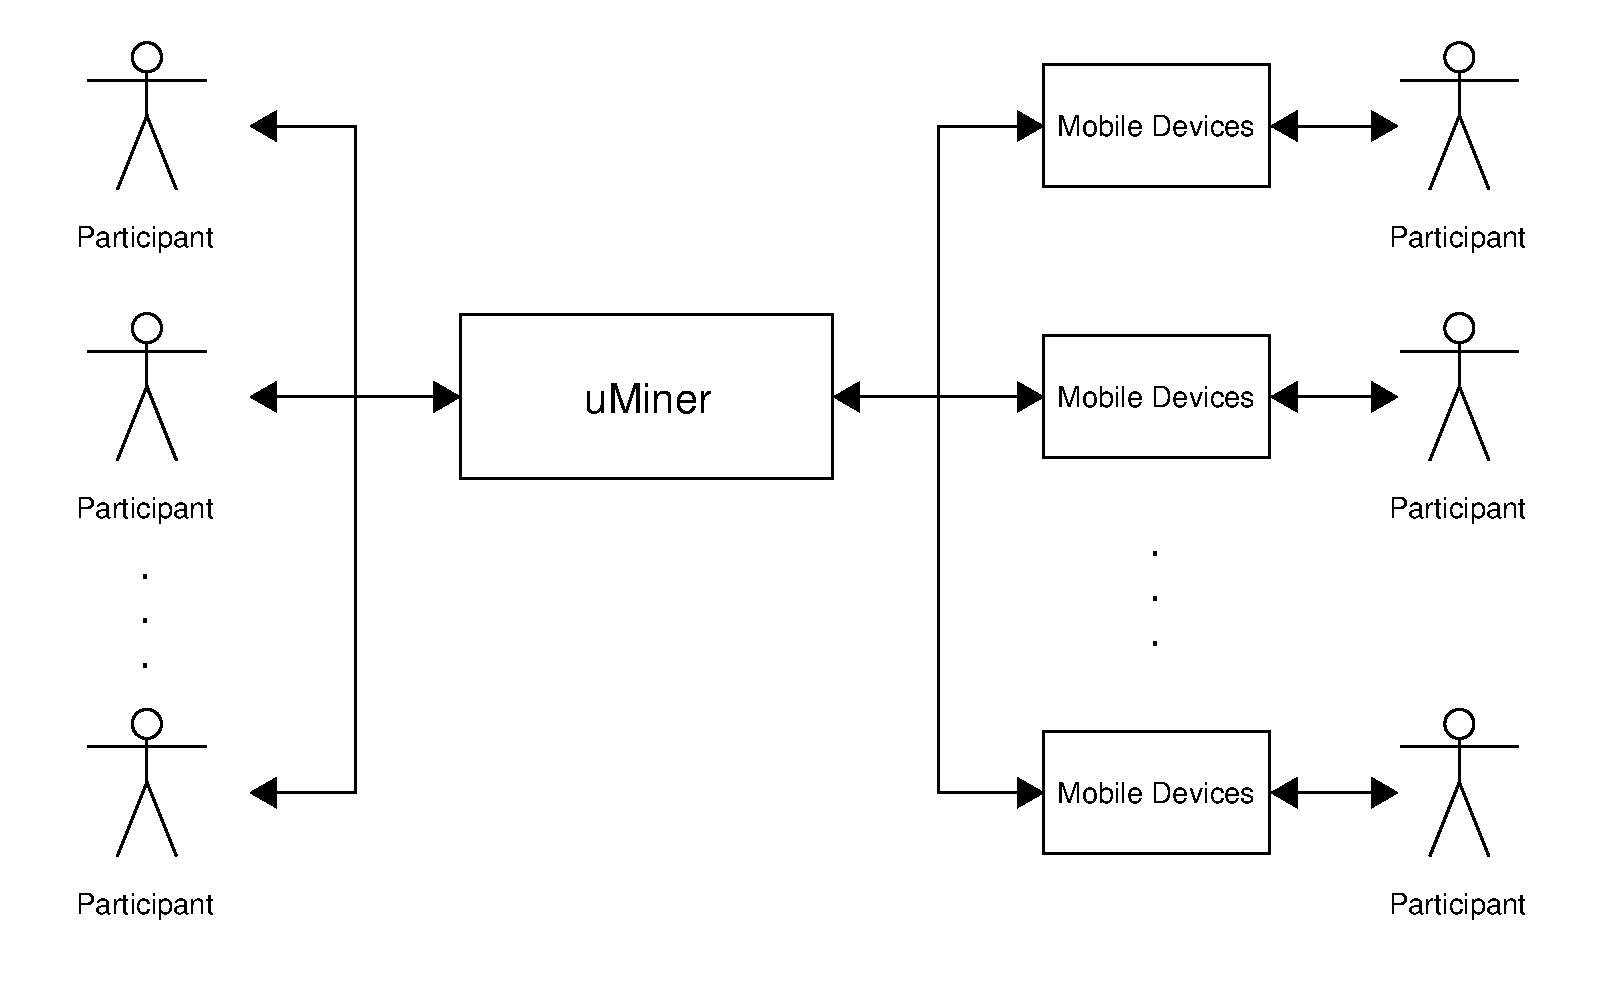
\includegraphics[width=0.8\textwidth]{problem_analysis/vision/system_vision}
    \caption{The system vision.}
    \label{fig:system_vision}
\end{figure}
\FloatBarrier

We imagine that our platform will handle all technical details related to the capturing of snapshots, and that customers should instead focus their effort on motivating participants to join their campaigns. 

\section{Delimitations}
\label{sec:delimitations}
From the vision scenarios, see \secref{sec:vision_scenarios}, we learned that the project could include profiles of participants, which could allow customers to target specific groups of people. We are certain the ability to target demographics would be valuable to customers, but we have however found this would significantly impact the implementability of our solution. We acknowledge the need for customers to have a more select group of people collect data. We have therefore; besides allowing participants to opt-in to campaigns, which we will refer to as public campaigns; decided to introduce a concept of private campaigns. A private campaign should work similarly to a public campaign, except that the campaign will not be listed publicly in the data gathering application. Access to a private campaign should be managed by customers, who would have to distribute an identifier for the campaign on their own. We feel confident that such a simple solution could provide some of the same value as including profiles of participants, while being easier to implement for first viable version of a solution.

% We could, besides sensors from mobile phones and wearables, also consider including external sensors such as cameras or smart home sensors like movement detectors or temperature sensors in the room. It is however demanding to support many different external sensors in an application, installation of compatible external sensors where the participants reside could entail high installation and maintenance cost and would require a different level of commitment from participants. There has been attempts to alleviate the burden of including many different external sensors in mobile applications by making it easier to interface with them and write drivers but the problem is still considered difficult and costly \parencite{open_data_kit}. We have chosen, at least initially, to not include external sensing as it is deemed too extensive to support collection of such sensors compared to the one of wearables and mobile devices.


%!TEX root = ../../super_main.tex

\section{Choice of Target Platform}
\label{sec:choice_of_platform}

\emph{uMiner} should give its customers access to as much training data as possible. Therefore we would like to have as many participants as possible involved in gathering the data. This means that developing a multi-platform mobile application would be ideal. There are different tools which can be used to create multi-platform applications, such as Xamarin or Adobe PhoneGap. Although they do it in different ways, both platforms enable developers to reuse code when developing mobile applications for multiple platforms, which in the end should save development time. 
\\\\
One problem is, that a large amount of our mobile application is focused around gathering data from the sensors of the devices, which varies a lot from platform to platform, meaning that we would have to somehow develop this code for each platform individually. Both PhoneGap and Xamarin require custom code to handle sensors for each platform, and Xamarin allows this better than PhoneGap does. 
\\\\
\todo[inline]{Læs om denne paragraf giver fin mening (corresponds til den gule lap der siger ``overvej om vi introducere Microsoft Band 2 lidt pludseligt'')}
Even though it would be possible to use Xamarin, we would not gain much from it, as we would have to write the code responsible for accessing the sensor outputs for each platform that we would support. Furthermore, we would have to spend time on learning to utilize a new framework for the development. We have instead chosen to develop an Android application using the native Java-based Android framework, which is a framework that we have used on a previous semester. Besides our previous experience with this framework, Android is also the ideal platform to work with due to its smartphone market share of around 80\% \parencite{android_os_market_share}, and the amount of wearables compatible with the platform. Furthermore, we have multiple Android devices available, as we have some ourselves, and as we can borrow Android devices from the university. The Android SDK and IDE, called Android Studio\footnote{http://developer.android.com/sdk/index.html}, are free and easy to setup and run on multiple platforms in contrast to many other options. We would like to include support for wearables in our project, and as we have a Microsoft Band 2 smart band at our disposal from the university, we have chosen to include it in our project.
\\\\
The Android operating system allows tasks to run in the background at all times, regardless of what developers intend to these tasks for. On the iOS platform, for instance, long-running tasks is only allowed for specific application types, such as audio playback and accurate navigation \parencite{apple_long_running_task}.
\\\\
The system should have a server solution that is able to store all the gathered information from the participants, and an interface for the customers to create and specify the campaigns they want. For this reason we have chosen the Laravel web framework based on the \textbf{P}HP: \textbf{H}ypertext \textbf{P}reprocessor (PHP) language. Laravel allows for routing and responding to various request. This will enable us to create a user interface for the customer, and a programming interface for the devices to communicate with. The Laravel framework does not have some obvious advantages over other web frameworks, however since some of the group member have previous experience with this particular framework, this will be the choice of platform for the server side of the system.

% \\\\
% On the Android platform there exist something called API levels which determines what version of the operating system that our application will be compatible with, we have chosen to support the API level 21, which is one of the most recent versions of the Android platform that is compatible with wearables. 

% Android er mest udbredte platform og de fleste wearables er nød til at være kompatible til
% Flest wearables der er kompatible med android
% Android har et helt økosystem til wearables, mens de 2 andre store kun har få til deres eget produceret ting
% Many wearables are depended on communication with a smartphone and a lot of wearables are compatible with Android. This is probably partially due to the fact that Android is the most used smartphone operating system \parencite{android_os_market_share} and partially because Android is also a an open wearable platform through Android Wear \footnote{https://www.android.com/wear/}.
% \\\\
% Vi har telefon til at teste på
% gratis og open-source/open-development environment
% We have Android devices available as we have some ourself and as we can borrow Android devices from the university. Android SDK and IDE, called Android Studio \footnote{http://developer.android.com/sdk/index.html}, is free and easy to setup and run on multiple platforms contrary to the Apple iOS development environment called Xcode \footnote{https://developer.apple.com/xcode/download/} which only runs on mac with OS X. We have not considered the Windows phone Operating system as a target platform because of its limited market share.
% \\\\
% We have therefore decided to develop the application, which should be run on the devices of participants, to run on the Android platform. On this platform there exist something called API levels which determines what version of the operating system that our application will be compatible with, we have chosen to support the API level 21, which is one of the most recent versions of the Android platform that is compatible with wearables. However, we had some issues in regards to this choice, both in terms of development method and some technical detailes regarding hardware and supported devices. A description of these issues and some reflection upon these can be found in \secref{sec:the_android_platform_compatibility_and_test_driven_development}.


\part{Feature Description} 
\label{prt:feature_ _description_}

% === ARCHITECTURE === %
%!TEX root = ../../super_main.tex

\chapter{Architecture}
\label{cha:architecture}

\todo[inline]{Describe the overall architecture of the system, such that it can be used as a basis for this part of the report, maybe move client-server architecture to here and maybe describe eco-systems of devices}
\todo[inline]{Describe the RESTful routes (how client and server communicates)}
\todo[inline]{Is this pretty and clear enough?}
\begin{figure}[!htbp]
    \centering
    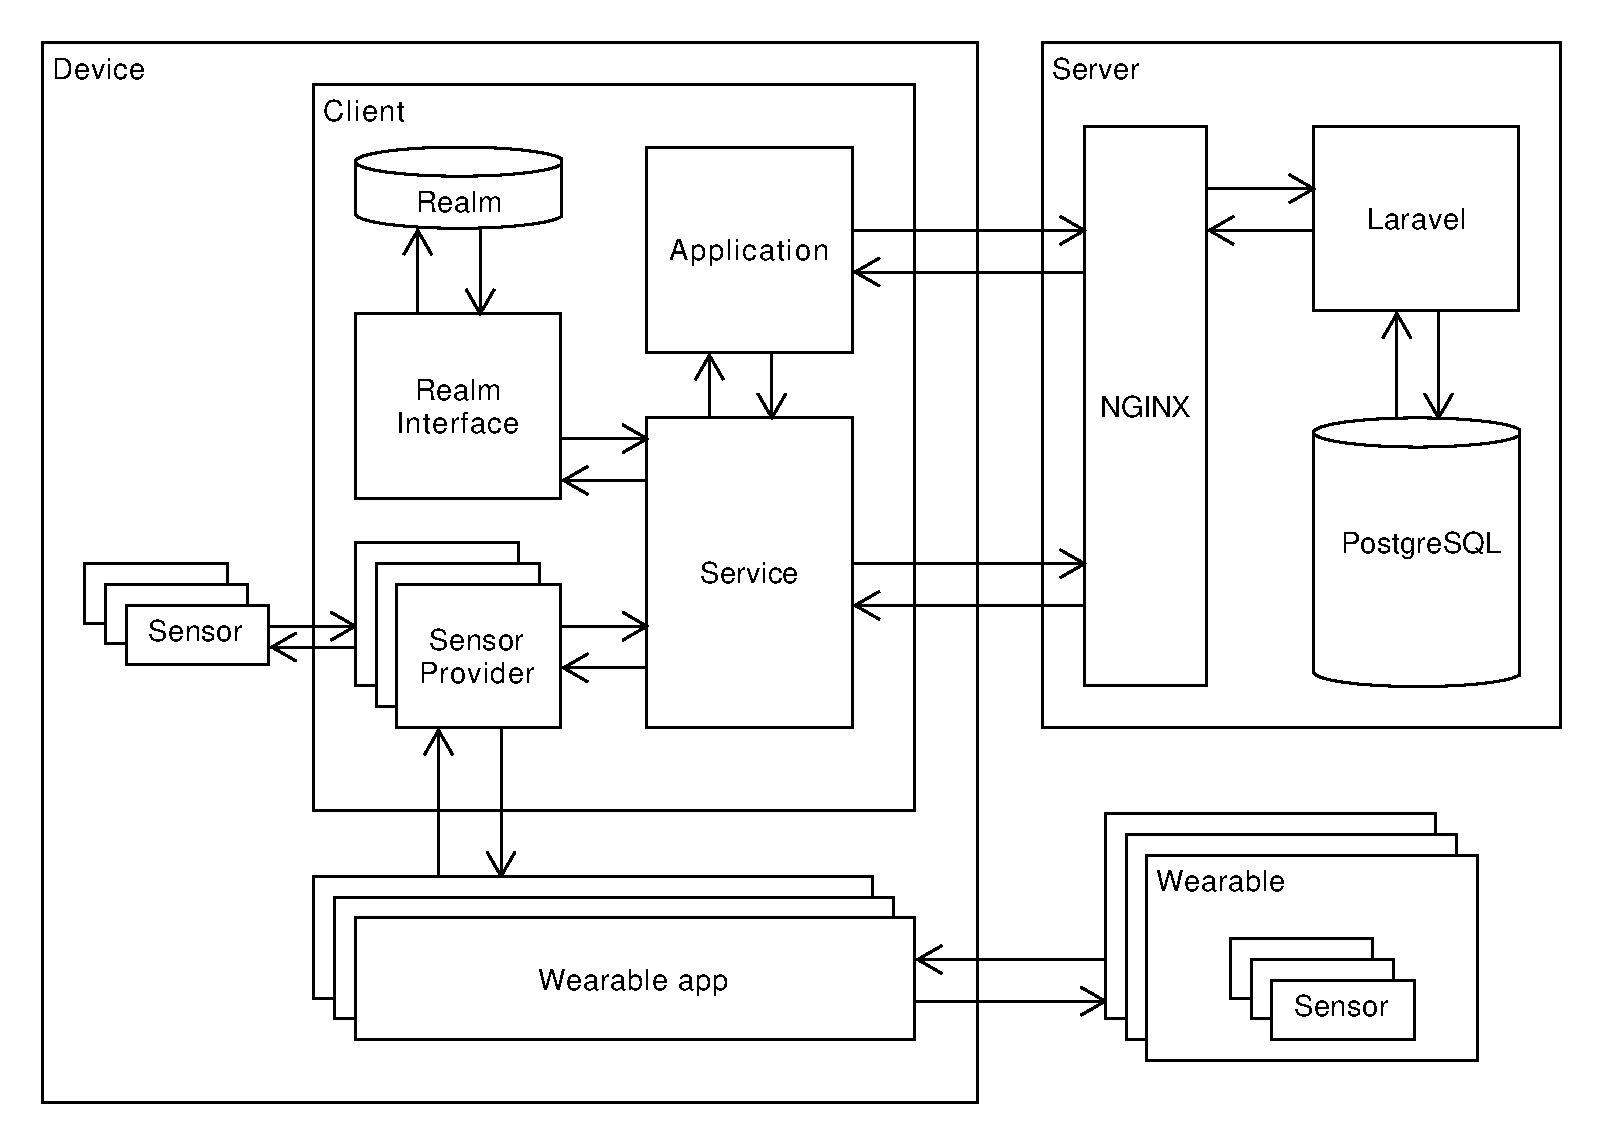
\includegraphics[width=\textwidth]{graphic/architecture/architecture.pdf}
    \caption{An abstract overview of the overall system architecture.}
    \label{fig:system_architecture}
\end{figure}
\FloatBarrier

%!TEX root = ../../super_main.tex

\section{Device}
\label{sec:device}
The device component is the part of the system that should run directly on the smartphone of the participant. This component is responsible for interacting with the participants, gather data from the sensors on the device, and communicating with the other devices in order to get data from wearables. The sensors represent the underlying hardware, and the Wearable Application is the interface from the client application to external wearable sensors, which in our case is the Microsoft Health application that communicates with Microsoft Band 2 we have implemented support for in the system.
\\\\
The client application contains a service component that is the main controller of the system client application. This service runs independently in the background at all times, and is the part of the system on a device that communicates with the different sensor providers, and also uploads the collected snapshots to the server. Furthermore it is also responsible for prompting the participants to answer the questionnaires. This service is completely detached from the interfaces, since it needs to ensure guarantees in respect to the real time aspects of gathering the sensor data.
\\\\
The UI components consists of two interfaces, a settings interface and a questionnaire interface. The settings interface allows for the participant to browse details and join campaigns. Furthermore, it also has some communication with the web server where it fetches the specifications of campaigns, and reports back to the server which campaigns the participants has joined. The questionnaire interface is a series of user inputs where the participants can provide answers for the questions of a questionnaire. This interface is prompted to the user by using notifications, which are sent by the service for every snapshot, in order to obtain labels on the data if possible.
\\\\
The service component is also in need of some persistent storage on the device, to ensure that it can store gathered snapshots, so that it can upload the data using best practices in regards of power consumption and robustness as described in \secref{sec:general_strategies}. For this reason the application has a storage module where we utilize a library called \mono{realm}, which will be further describe in \secref{sub:local_storage}.
\\\\
Lastly the service component is heavily dependent on the sensor providers, which are providers that abstracts various types of sensors, for example hardware sensors on the device, software sensors, and external sensors from wearable and so on. From the service point of view, it only needs to manage the specification of campaigns and request the data from these providers accordingly before it stores the data that has been gathered from these providers on the device. The controller of the service assumes that the interface of these providers guarantees the amount of data requested and that they keep their deadlines in regards to timing of measurements.

%!TEX root = ../../super_main.tex
\section{Server}
The server provides the interface for the customers of the system, the ones in need of campaigns. Besides allowing the customers to specify campaigns the, server is also responsible for handling the upstream of snapshots from the devices of the participants. Meaning that the server has both a application programming interface (API) \todo{check if this is the first place we mention API} and a graphical user interface (GUI) \todo{check if this is the first place we mention GUI} for the customers. The server runs a web server technology called NGINX which handles the network communication using the hyper text transfer protocol (HTTP) \todo{check if this is the first place we mention HTTP} and allows for using transport layer security (TLS) \todo{check if this is the first place we mention TLS}. Furthermore this web server is also able to communicate with the underlying operating system to be able to read files from disk and interpret PHP code.
\\\\
With these features of NGINX the server is now able to facilitate the web framework Laravel. This framework builds on the model-view-controller (MVC) pattern. This allows us to route incoming requests and handle them as both application request but also as user requests. 

\todo[inline]{Snak om PostgreSQL}


% === SECURITY === %
%!TEX root = ../../super_main.tex

\chapter{Security}
\label{cha:security}

Since the system should be able to handle personal data, there are certain security constraints that we must comply with as described in \secref{sec:personal_data}. For one the legislation states that the personal data must be encrypted at all times, constraining that all ways these data are communicated must also be encrypted. For this reason we utilize an encrypted network protocol (HTTPS) using SSL encryption.

%!TEX root = ../../super_main.tex

\section{Secure Socket Layer}
\label{sec:secure_socket_layer}

Secure Socket Layer (SSL) is a broadly used security technology for creating a secure connection between a client and a server. SSL establishes this secure connection by utilizing both symmetric and asymmetric encryption. Symmetric encryption algorithms use the same encryption key for both the encryption and decryption of the communication, whereas asymmetric encryption encrypts the communication using one key (a public key) and decrypts it using another (private key). 
\\\\
\todo[inline]{Har svært ved at finde en god/akademisk kilde til det her}  
To establish the connection between the client and the server, the client initially sends the server information of how it wishes to communicate, such as what version of SSL/TLS, what cipher suites it supports and how the messages between them should be validated. The server will then chose what version and what algorithms are used in the communication and send it back to client along with its certificate and its public key. The client will then validate the certificate through a Certificate Authority (CA). If it is valid the client will use the public key to encrypt a \mono{PreMasterSecret} that will be used by both the client and the server to create the key for the symmetric encryption algorithm that will be used for further information. The key will be based on both the \mono{PreMasterSecret} as well as some random numbers that have accompanied every request up to this point. The server will then decrypt the \mono{PreMasterSecret} using its private key. The server and the client can then both generate the key used for the symmetric encryption algorithm based on the random numbers and the \mono{PreMasterSecret} and use this for any further communication.
\\\\
For our purposes we have chosen to use what is called a self-signed certificate, because it covered the need for encryption that we had, and the price of a certificate issued by a CA is fairly high. The certificate we use was created by using OpenSSL\footnote{https://www.openssl.org}, which is an open source project that allows you to create your own certificate. One of the issues in utilizing a self-signed certificate is that the certificate will not be trusted by most browsers and operating systems. A more severe problem is the fact that it leaves the connection vulnerable to a man in the middle attack, where a third party with malicious intent might intercept the connection and use his own ``fake'' certificate and thereby getting access to potentially sensitive information. This would not be a problem if we had used a certificate issued by a CA, because the certificate then could be validated. Having a self-signed certificate also means that most browsers will not trust the certificate, and make the user of the browser aware that the site they are trying to connect to might be insecure with a scary warning page. 
Another problem is that the self-signed certificates are not trusted by Android, which causes problems when trying to make a connection to our server. To solve this problem Android provides the possibility of overriding what they call their \mono{TrustManager}, which we have done. 

\todo[inline]{insert snippet of trust manager override, and explain it above}

Another problem that we encountered with the Android platform is that there are issues when a certificate uses what is called wildcard subdomains. Wildcard subdomains allows us to use the same certificate for various subdomains. The reason why it is necessary for us to have multiple subdomains is that we have a development site (dev) and a production site (prod). These sites all should have different domains to allow the server to tell them apart. Furthermore, the server has different IP addresses depending on if the server is accessed from the university network, or if it is accessed from outside, meaning that we need different DNS records for in house access and outside access. Therefore we created the different DNS records seen in \tabref{tab:dns}, and used the wildcard domain ``\mono{*.*.ourdomain.dk}'' on our certificate.

\begin{table}[!htbp]
	\centering
	\begin{tabular}{|l|l|} \hline
		\textbf{Domain}				& \textbf{IP}	\\ \hline
		prod.local.ourdomain.dk 	& localip		\\ \hline 
		dev.local.ourdomain.dk 		& localip		\\ \hline
		prod.global.ourdomain.dk 	& globalip		\\ \hline
		dev.global.ourdomain.dk 	& globalip		\\ \hline
	\end{tabular}
	\caption{DNS records}
	\label{tab:dns}
\end{table}

In case of wildcard subdomains the standard Android hostname verifier will try to check if the domain is an exact match to the requested hostname, which will fail and raise an exception. Luckily, the framework allows us to override their \mono{HostnameVerifier} as seen in \todo{insert hostname verifier ref}

\todo[inline]{Insert snippet of hostname verifier and describe it below}

Having the server placed on the university did also introduce other problems, due to a limitation in what ports that we could use for outside access. 
We were assigned two different ports from outside access namely port 8000 and 8001, which we used for the web application, and our continious integration system respectively. 
If we had access to the ports normally used for the HTTP and HTTPS protocols, we could have used a system called let's encrypt \footnote{https://letsencrypt.org}, which is an free certificate authority trusted by all major browsers \parencite{lets_encrypt_all_browsers}. Let's encrypt allows for automatic verification of domain name ownership by installing their client on the server, where it will use port 80 and 443 to access validate a servers authenticity and create a certificate that can be validated through them. Using let's encrypt as our CA would remove the intimidating error potential customers encounter when accessing our page through most web browser, and also remove the need for overriding the \mono{HostnameVerifier} and the \mono{TrustManager} in the Android client code.

%!TEX root = ../../super_main.tex

\section{Storage Encryption}
\label{sec:storage_encryption}
% Skriv om at vi skal gemme data sikkert
According to the legislation briefly described in \secref{sub:legislation}, data that can identify individuals must be encrypted. In our case we both need to store data locally on the clients Android device, as well as remotely on a server dedicated to storing the data and showing it to the correct customers, meaning that we will have to consider security and encryption in two different code bases and on two different platforms. 

\subsection{Local Storage}
\label{sub:local_storage}
We decided to look at different options to ensure, that we could safely store the gathered data on Android devices. Storing the data locally requires a local solution for encrypting all saved data in persistent storage on a device. 
\\\\
Firstly, we considered the SQLite DBMS which is natively supported on the Android platform. The problem with using SQLite is that we would have to create a schema for each of the sensors and their data types, making it a longsome task. The process of adding new sensors would also become more tedious, making the system less adaptable to new sensors. Furthermore to ensure encryption on a SQLite database we would have to use an extension to SQLite called SQLCipher\footnote{https://www.zetetic.net/sqlcipher/} which would allow us to encrypt the database. 
\\\\
Another option that we looked at is Android-Simple-Storage (ASS)\footnote{https://github.com/sromku/android-simple-storage}, which, as the name implies, is a simple library for handling the internal (storage reserved for an application and only accessible through the application it is reserved for) and external (SD card or other shared storage) storage in Android. ASS allowed us a simple interface to this file system while at the same time it made it possible to encrypt the data directly through the library by specifying a few options. We therefore implemented a prototype of this as our main storage for the application. Our prototype was based on JSON as our file format and the GSON library, which provides easy serialization and deserialization of Java objects to and from JSON. A problem arose with this approach. This way of storing our data could not pass one of our acceptance tests stating that:

\begin{itemize}[noitemsep]
   \item When there exist a snapshot model, which does not use more than 0.42 MB storage space using all sensors (per device) for one hour
   \begin{itemize}[noitemsep,topsep=0pt,parsep=0pt,partopsep=0pt]
      \item Snapshot duration: one hour
      \item Sample frequency: one minute
      \item Sample duration one second
      \item Measurement frequency: 100 milliseconds
   \end{itemize}
\end{itemize}

The problem was that we used more than the maximum storage size of 10 MB as stated in the acceptance test. The JSON format had too much overhead, because it utilizes explicit field names instead of a schema, and thus it used more storage space than what should be needed. 
\\\\
This lead us to explore other options, and we came across Realm\footnote{https://realm.io/}. The developers behind Realm says that it should be the replacement for SQLite, and that it should not just be an Object Relational Mapping (ORM) on top of it. Realm uses its own persistence engine, and is cross-platform meaning that the same Realm file can be shared across multiple platforms. Realm natively supports encryption of the data. We ended up choosing Realm for our persistence layer. One of the drawbacks of Realm is that it only supports a single level of inheritance to specify which objects should be able to be stored persistently. All persistent objects must directly be children of a class called \mono{RealmObject} and it is therefore not possible to create complex inheritance hierarchies with multiple levels of inheritance with abstract classes to help minimize code duplication.  
\\\\
Another drawback is that Realm only supports one aggregate or collection type, namely \mono{RealmList}. Realm does not support types such as maps or enums, forcing us to either serialize and deserialize objects of these types manually or by creating class wrappers that extends \mono{RealmObject}, which could represent the unsupported types.

\lstinputlisting[
   style = Java,
   caption = {An example of how the realm is accessed and objects in it are manipulated.},
   label = {lst:realm_example},
   float=!htbp,
]{content/security/code_snippets/notifyQuestionnaireCompleted.java}
\FloatBarrier

\todo[inline]{Rikke: This text need some rework, it is quite difficult to understand}
Realm still has a nice API even though has these restrictions. A realm configuration is needed to create a realm instance. Different parameters can be set for a realm configuration such as an identifying name and whether data should be encrypted. One can obtain a previously defined default instance of the access point, simple called a (\mono{realm}), as can be seen on \lineref{lst:get_default_realm} in \lstref{lst:realm_example}. It is then possible to obtain objects of certain types by using the obtained instance. We are in this case looking for a \mono{Snapshot}, where its timestamp is equal to a given value. In this example we want to add a questionnaire with its questions answered to the snapshot, in the case such a snapshot exists, by first adding it to the realm, and then update the snapshot with the given questionnaire set as a field on the snapshot. Similar to the \mono{copyToRealm} and \mono{copyToRealmOrUpdate} there also exists functionality for removing objects from a realm, namely \mono{removeFromRealm} and \mono{removeAllFromRealm}.
\\\\
Realm creates a schema for the application based on compile time language reflection of classes and language supported annotations of class members. Realm looks a at all direct subclasses of \mono{RealmObject} and at annotations such as \mono{@PrimaryKey}, for specifying the member which should work as the primary identifying key; and \mono{@Ignore}, which tells Realm to ignore a given member when creating the schema.
\\\\
The default configuration used in the previous example needs to be set somewhere, as mentioned, before any access is attempted from the application. The code responsible for setting the default instance can be seen in \lstref{lst:realm_default}. 

\lstinputlisting[
   style = Java,
   caption = {The algorithm generating encryption keys.},
   label = {lst:realm_default},
   float=!htbp,
]{content/security/code_snippets/setupRealmAndStartTimers.java}
\FloatBarrier

The code for specifying an instance of a realm, as shown, is very simple, and a thing such as encryption is handled by just a single line of code, given that the encryption key is known at this point. How we generate and retrieve the encryption key is covered below. 

\subsubsection{Encryption Keys}
\label{sub:encryption_keys}
A requirement when storing sensitive data encrypted is that the encryption key is not stored on the same unit as the data. We initially stored the encryption key in the source code of the application to simplify the encryption of the data. A problem with this approach, and the reason why it is a requirement to store it separately, is that a distributable application, known as an APK file, which is made publicly available, can be decompiled and the encryption key could potentially be extracted. 
\\\\
All that is needed for a potential attacker or malicious application is then to somehow gain access to the internal storage of our application and fetch the Realm file. The internal storage of the application is private, and under normal circumstances the underlying Linux operating system will only grant the application owning the internal storage access to it. This holds unless there is a security hole present, or the user of the device has rooted his device, i.e. is using a privileged account, in which case it is possible to access the internal storage of every application on the device. An application or user with root privileges could then access our storage and with the use of the key found in the decompiled APK and gain access to all the sensitive information that we store on the device.
\\\\
Instead of storing the encryption key on the device we decided to move it to the server, and also ensure that every device has its own encryption key. Having an encryption key for each device requires us to somehow be able to uniquely identify a device. Luckily, as mentioned in \secref{sec:device_identification} we have a way of generating a unique identifier for each individual device. In having the device identifier it is possible for us to generate a 512 bit random encryption key the first time a device issues requests to our server and then simply return the newly generated key or a stored key if one has already been generated for the given device. This key exchange is of course done over our TLS encrypted connection covered in \secref{sec:transport_layer_security}. We generate the key with the algorithm seen in \lstref{lst:encryption_php}. 

\lstinputlisting[
   style = PHP,
   caption = {The algorithm on the server generating encryption keys.},
   label = {lst:encryption_php},
   float=!htbp,
]{content/security/code_snippets/encryption.php}
\FloatBarrier

This algorithm utilizes the random number generation features in the Linux kernel, by utilizing a special file, \mono{/dev/urandom} that interfaces the random number generation. Each time this file is read by the algorithm it will return a random byte, making it ideal to generate a sequence of random bytes representing an encryption key. The algorithm firstly create a file pointer to the \mono{/dev/urandom} file with the \mono{fopen} function. The function will return \mono{FALSE} if the file could not be opened, which is checked in \lineref{lst:fp_check}. Next, we will read the number of specified random bytes with the \mono{fread} function, which we will then return back to the call site as a binary string. This key can then be sent to a client if requested. On the Android client the encryption key is expected to be in the format of a byte array, meaning that we will need to convert the binary string into such a data structure. 
\\\\
Luckily, the library that we utilize for making HTTP requests from the Android application has built in support for conversion of binary data into byte arrays very simple as shown in \lstref{lst:binary_to_byte_array}, where we simply send a GET request with the \mono{device\_id} as a parameter. The request that is send will be sent up to three times if the transmission fails, which is specified with the \mono{retry(3, false)} method call. Lastly we utilize the asBytes method to transform the response that we get to a binary array, which is what the body type of the response then will resolve to in the \mono{onResponseCodeMatching} method. In this method we simply can get the converted response body corresponding to the encryption key generated by the server, and utilize this throughout our application to encrypt and decrypt the realm file.    
\lstinputlisting[
   style = Java,
   caption = {Simple example of how we use the Webb library to convert binary strings to an byte array.},
   label = {lst:binary_to_byte_array},
   float=!htbp,
]{content/security/code_snippets/getEncryptionKey.java}
\FloatBarrier

\subsection{Remote Storage}
\label{sub:remote_storage}

According to the legislation the data on the server should also be encrypted. However, due to limited limited time and prioritization of functionality over security, we have not been able to implement proper encryption of the data on the remote storage. We are utilizing PostgreSQL and it has some support for encryption that may fit our needs, however, the connection to the database is currently managed through an ORM, which might complicate the task of decrypting the data before it is used in the application. To be able to release this product we would have to implement encryption on the back end as well to meet the statutory demands.



% === GATHERING SENSOR DATA === %
%!TEX root = ../../super_main.tex
\chapter{Gathering Sensor Data}
\label{cha:gathering_sensor_data}

A core feature of uMiner is the ability to gather sensor data from the participants' devices. This chapter describes how this data is structured, but also how we handle the gathering of sensor data concurrently. Furthermore, the chapter will cover some of the measures we have taken to minimize the network and battery impact of the Android application.

%!TEX root = ../../super_main.tex

\section{Structuring Sensor Data}
\label{sec:modeling_sensor_data}

\todo[inline]{Skriv en blød introduktion der beskriver hvorfor vi har brug for en god struktur.}

Conceptually, a \emph{snapshot} is a snippet of the reality (context) that a specific participant exists in, measured through the participants' devices, along with a \emph{label}, describing the context further. This label is used to define the context in ways that available sensors cannot. By examining the measured context and the labels describing these measurements, customers will be able to search for patterns in the data, and thereby might be able to see a correlation between sensor output and human dynamics. To search for temporal patterns in the data collected from the continuous- and reactive sensors, covered in \secref{sec:deriving_the_context_from_sensors}, multiple measurements are required. An example of this could be measuring the location of a participant over time to see that a user is moving. To facilitate this, a snapshot consists of a sequence of sensor readings collected from multiple sensors and a label. In order to see this development over time, time has to pass between every measurement. This timespan depends on what the customer desires to measure, and therefore he/she must be able to configure how long a delay there should be between every sensor reading. To define this timespan, and other aspects such as which sensors to measure from, and when to present the questionnaire to the participants, the customer must define a \emph{campaign}.
\\\\
One could imagine that a customer might be interested in finding a correlation between heart rate, movement patterns, and the influence of alcohol. In order to do this, a customer could create a campaign, in which he specifies which information should be gathered from the sensors, such as heart rate, acceleration, and GPS location. The customer would furthermore specify questions for the participants, asking whether they are, or have been, under the influence of alcohol at a specific time. One could alternatively utilize a breathalyzer, but these are not common in mobile devices, making a questionnaire a viable alternate method for distinguishing if the participant have consumed alcohol. When contributing information to this campaign, participants would submit snapshots matching this specification. An illustration of how these snapshots are structured can be seen in \figref{fig:snapshot_model_no_samples}, which shows how time elapses between every measurement. In this example, the participants are asked to answer the question: \emph{Are you under the influence of alcohol?} in order to label the data.
\\
\begin{figure}[!htbp]
    \centering
    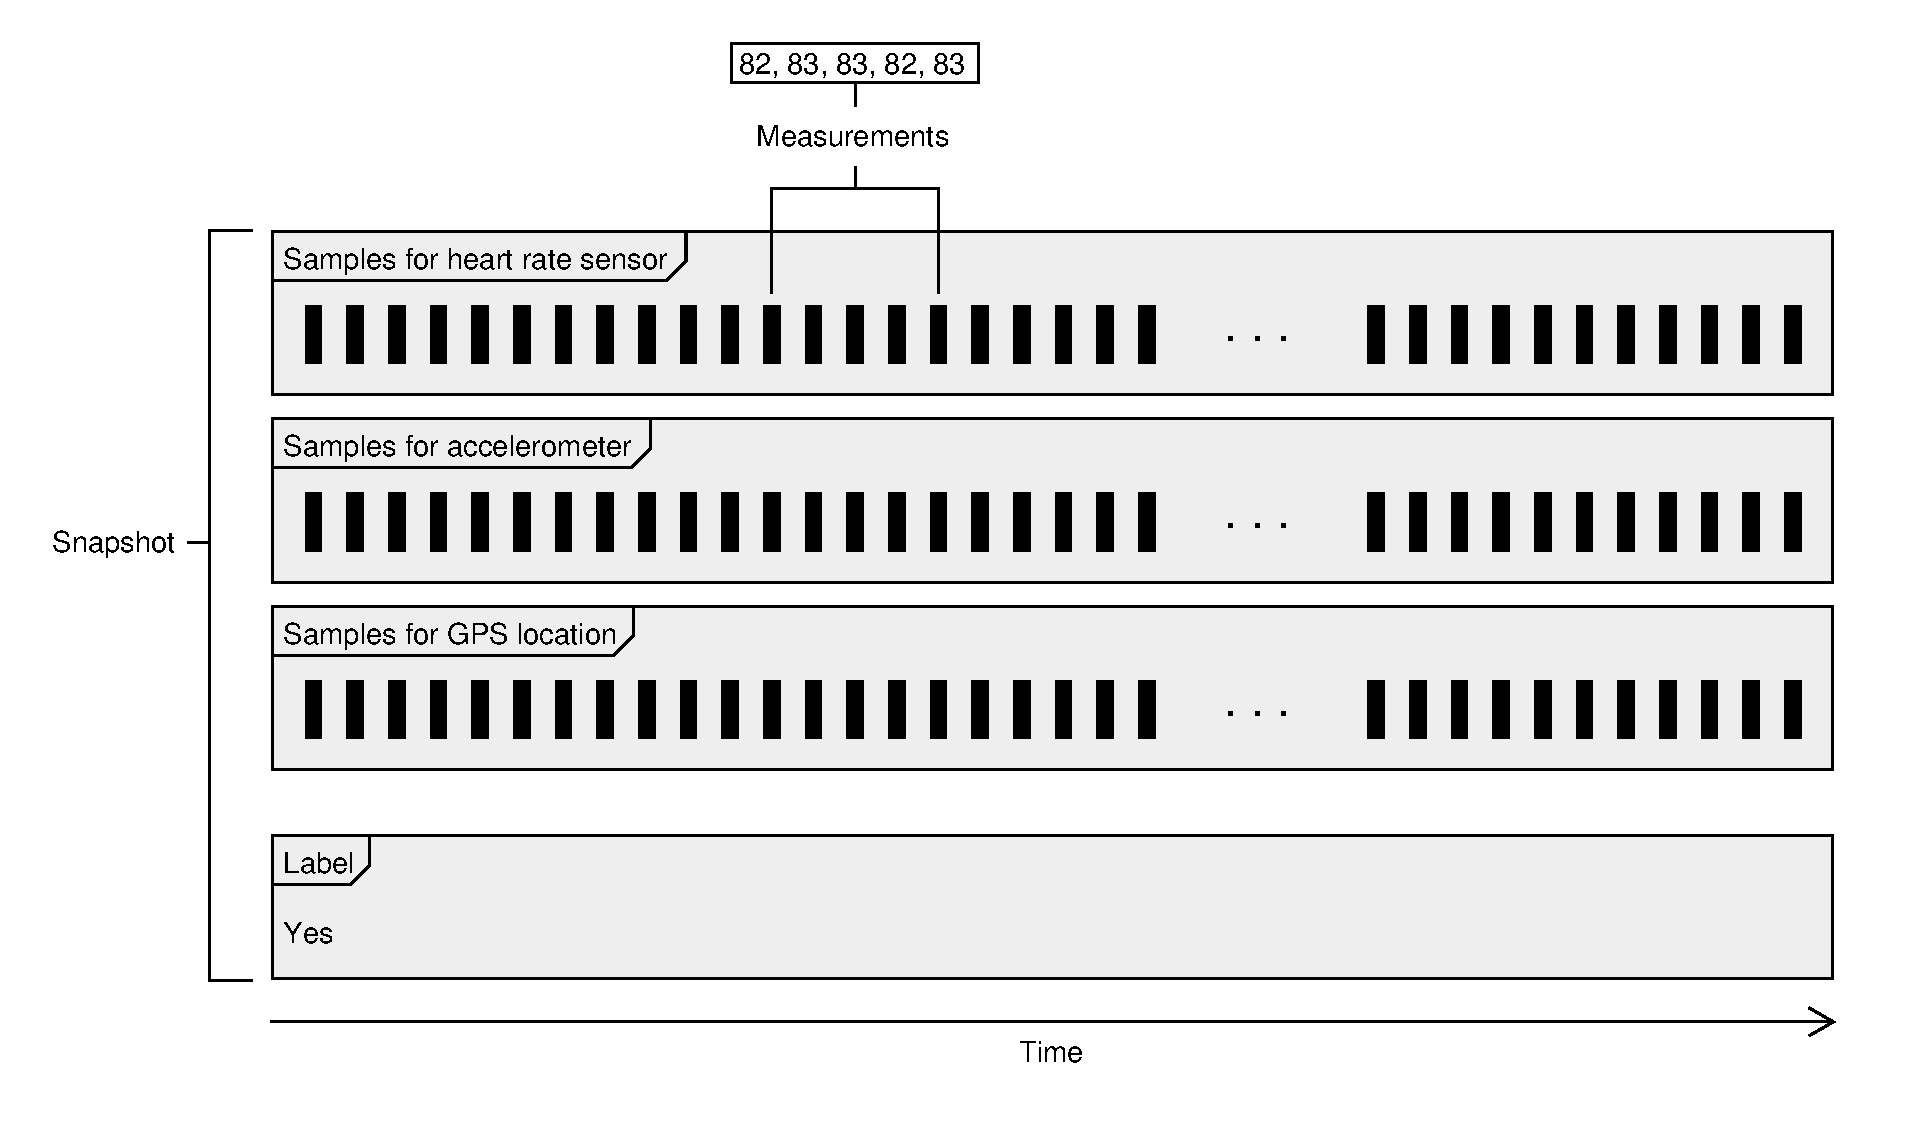
\includegraphics[width=\textwidth]{gathering_sensor_data/snapshot_model_no_samples}
    \caption{Snapshot example containing measurements from three sensors and a label.}
    \label{fig:snapshot_model_no_samples}
\end{figure}
\FloatBarrier

%!TEX root = ../../super_main.tex

\subsection{Data Quantity Estimation}
\label{sec:data_quantity_estimation}
%This gave us a dataset with a size of 142908 bytes. This experiment would then yield a data set of approximately 205 MB if it was run for a day. Running the same experiment for 30 days with 100 different devices would then approximately yield a data set of 617 GB assuming similar mobile devices with similar sensors. This quick napkin math was only for one sensor with 100 people and this could quickly escalate if more sensor or more people are added.

\todo[inline]{Overvej: Lav en reference til vores user story, og fortæl hvor meget data vi samler om dagen med disse målinger. Skriv også at dette KUN er RÅ sensor output, stored i Java-hukommelse størrelser. Med snapshot struktur er det meget værre} 

According to our problem statement in \secref{sub:problem_statement}, we want to minimize the effect that our application has on the  daily mobile lives of participants. One aspect that might have influence on this is the battery consumption and network usage of our application. We would there like to minimize these factors. In order to do this, we have experimented with different continuous sensors on a Nexus 5 smartphone and logged all values captured from the sensor for 1, 5, and 20 minutes. The results of these tests can be seen in \tabref{tab:sensor_experiment}. Note that the orientation sensor is a virtual sensor, which uses data collected from both the gyroscope and magnetometer, hence the correlation between the data sizes ($143 \text{KB} + 35 \text{KB} \approx 177 \text{KB}$ for 1 minute). These tests were only performed for four different sensors, but customers might need data from several different sensors, thus further increasing the amount of data collected. These quantities of data might present a problem even on modern mobile platforms due to paid limited data plans and battery consumption. There might be different data needs, some customers might require very detailed data from many sensors from a few devices and others might require more sparse data from a few sensors from a lot of different devices. However, we can conclude that gathering a continuous stream of data from all sensors all the time is not a viable solution.

\begin{table}[!htbp]
\centering
\begin{tabular}{l|c|c|c|c}
\textbf{Sensor}     & \textbf{Accellerometer} & \textbf{Gyroscope} & \textbf{Magnetometer} & \textbf{Orientation} \\ \hline
\textbf{1 minute}   & 142 KB                  & 143 KB             & 35 KB                 & 177 KB               \\ \hline
\textbf{5 minutes}  & 714 KB                  & 714 KB             & 178 KB                & 892 KB               \\ \hline
\textbf{20 minutes} & 2,859 KB                & 2,859 KB           & 715 KB                & 3,573 KB                
\end{tabular}
\caption{Data size of sensor data collection after a set amount of time.}
\label{tab:sensor_experiment}
\end{table}
\FloatBarrier

\subsection{Temporal Properties of Snapshots}
\label{sec:temporal_properties_of_snapshots}

\todo[inline]{Skriv en opdateret introduktion der er baseret på \secref{sec:data_quantity_estimation}, der forklarer hvorfor vi har behov for samples, og deres delay. Det er IKKE fordi kunderne synes at det er godt!}

\todo[inline]{Beskriv konflikten mellem customers og participants (kunder vil gerne have meget data, men participants kun vil give så lidt som muligt).}

\todo[inline]{Beskriv at det er et krav at mellemrummet mellem measurements er konstant, så vi kan sammenligne measurement på index x i et sample for sensor 1, sammen med index x i et andet sample for sensor 2. Alternativt kunne man tage et timestamp på alle measurements, men det vil tage meget plads at sende, så istedet vil vi gerne have et timestamp på sample, og en relativ tid på measurements.}

A single sensor reading from a continuous sensor often does not make much sense on its own, which is why we introduced the \emph{measurement} concept. Following the introduction of measurements, we came to the realization that customers might be interested in taking a stream of measurements, waiting for some amount of time, and then taking another stream of measurements. The customers might need data sequences that is separated by some span larger than the one between measurements. However, the more apparent benefit of this is to encourage the participants to join, due to reduced strain on their hardware. In introducing a span between a sequence of measurements the customer can regulate this in order to reduce the amount of data send to the server, which will reduce the battery and network consumption on the participants' devices. This has led to the introduction of a concept that we call \emph{sample}. A \emph{sample} is simply a sequence of \emph{measurement}s with an interval between them, as seen in \figref{fig:snapshot_example_with_samples}. This allows customers to make sense of continuous sensor readings, but in a periodic manner, that avoids unnecessary strain on the participants' devices.

\begin{figure}[!htbp]
    \centering
    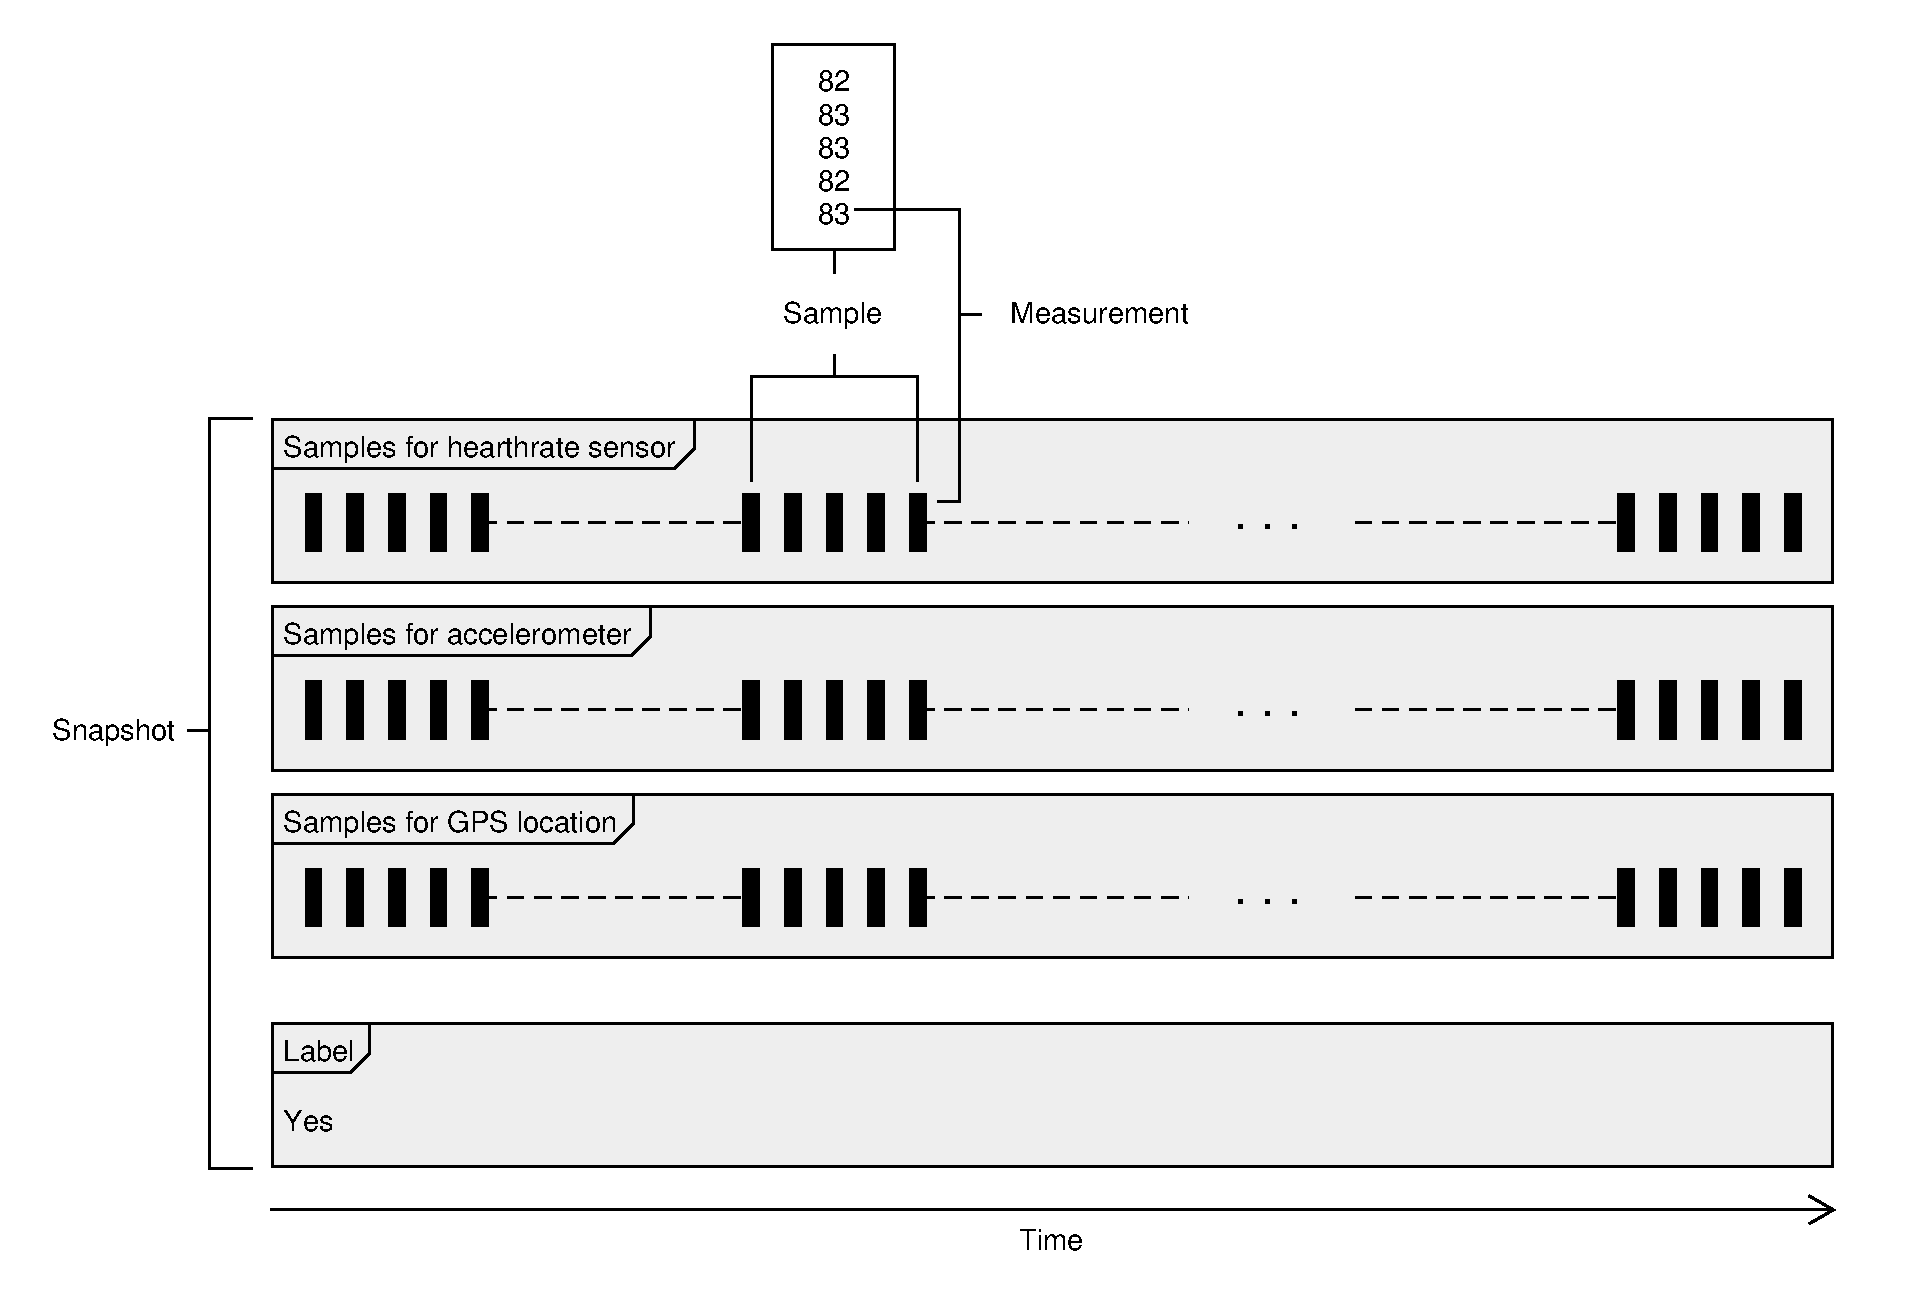
\includegraphics[width=\textwidth]{gathering_sensor_data/snapshot}
    \caption{Snapshot example containing samples from three sensors and a label.}
    \label{fig:snapshot_example_with_samples}
\end{figure}
\FloatBarrier

We want customers to configure how often \emph{measurement}s should be made, and we therefore allow them to define a \emph{measurement frequency} for their \emph{campaign}. Customers should furthermore be able to define how often \emph{sample}s should be gathered, and for that reason we allow them to define a \emph{sample frequency}. Lastly, the length of the \emph{snapshot} is configurable by defining how many \emph{sample}s the customer wants for a single \emph{snapshot}. This is used to calculate what we call \emph{total duration}, which states for how long samples should be generated for a snapshot. All of this is illustrated in \figref{fig:sample_temporality}. 

\todo[inline]{Skriv hvordan label'en kommer ind i billedet. Det skal forklares i dybden, og ikke bare være en sidenote
. Før stod der: Lastly, a customer should be able to define when the questionnaire should appear to the participant, for example at the start or the end of a snapshot.}

\begin{figure}[!htbp]
    \centering
    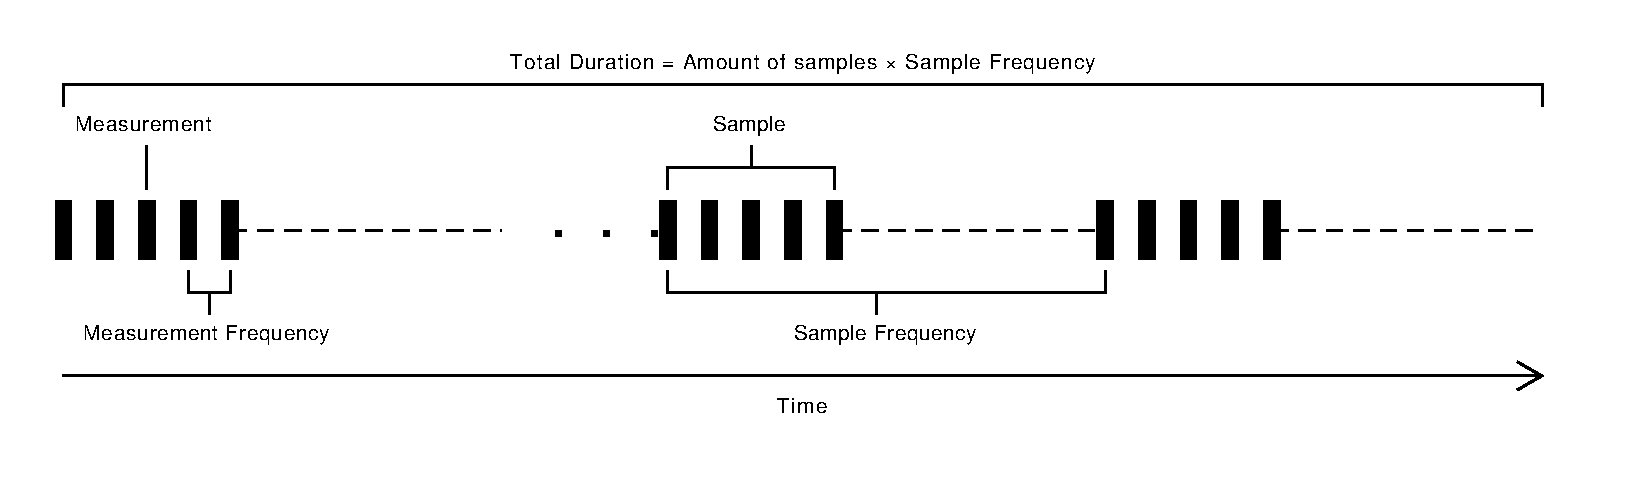
\includegraphics[width=\textwidth]{gathering_sensor_data/sample_temporality}
    \caption{Illustration of temporality for samples for a single sensor in a snapshot.}
    \label{fig:sample_temporality}
\end{figure}
\FloatBarrier

By this temporal structure of the sensor data we provide a viable way of configuring how the snapshots should be structured in regards to sensor readings, while maintaining a uniform output format for customers of the system.


%!TEX root = ../../super_main.tex

\section{Providing Sensor Data}
\label{sec:providing_sensor_data}

To support this structure of the sensor output, we have designed an abstraction over the different sensors available. This abstraction is designed for concurrent collection of samples, as we want the application to be able to gather information from multiple sources at the same time, meaning that the system is able to, for instance, collect data regarding the motion and location of the participant simultaneously. This is done in order to make sure that the gathered data is obtained according to the desired temporality of the customer, i.e. the time constraints of the campaign.
\\\\
Problems will arise when enforcing temporality of snapshots due to the event oriented nature of sensors in Android. Sensor events will trigger whenever a value is updated. This effectively means that it is impossible to know when these events will trigger. We want to guarantee that measurements can be made with a specific frequency independent on what is supported by the sensor, i.e. measurements can be made more often than what some sensors provide, but also more rarely. To make it possible to always get samples at the desired rate, we need to store the last measured value. To do this, we will use a cache, containing the last measurement. This concept is illustrated on the message sequence diagram in \figref{fig:cached_values}. If multiple values are output from the sensors in between two sample readings, only the latest one will be considered by the sample collection unit. This might mean that some sensor readings will not be used for anything, but this is a necessary precaution we have to take, in order to ensure the temporal features of the snapshot. In the case where no measurements have been provided by the sensor, and the sample collector reads the cache, a default value will be read, which will reflect the fact that no measurements have been provided. It is then up to the customer to handle this.

\todo[inline]{Rikke: Need to explain the figure better}
\begin{figure}[!htbp]
    \centering
    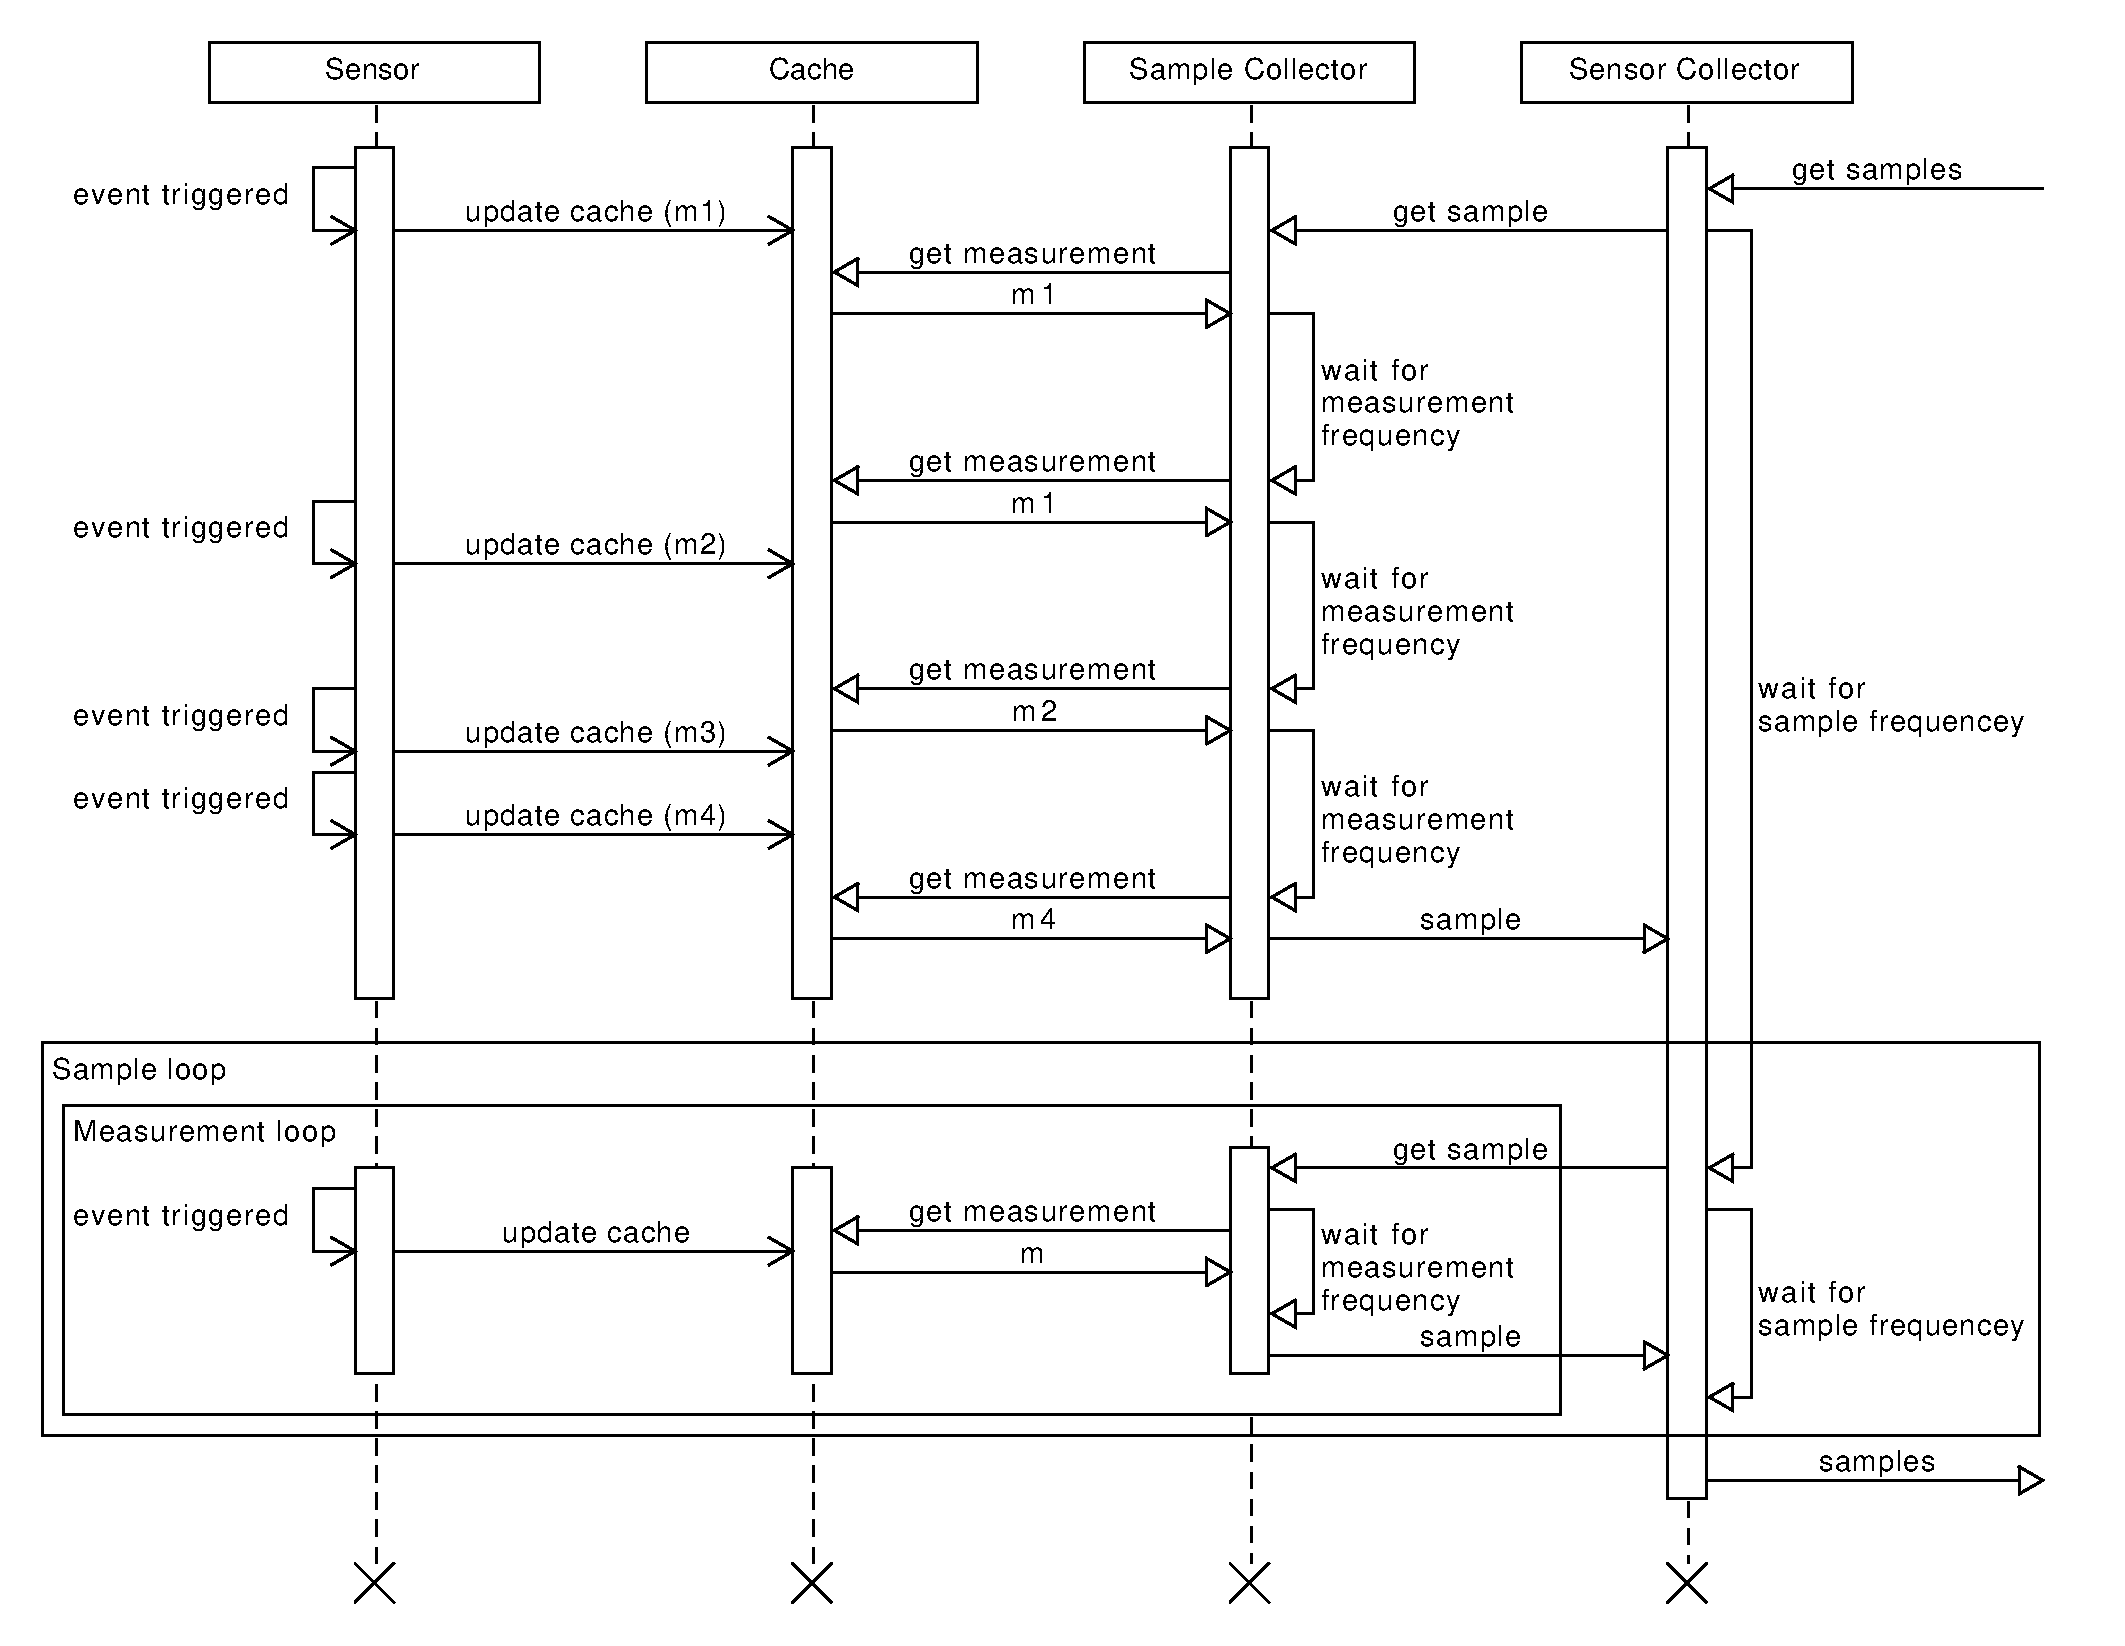
\includegraphics[width=\textwidth]{backgroundsensorservice/cached_values}
    \caption{Snapshot creation based on cache to ensure desired temporality.}
    \label{fig:cached_values}
\end{figure}
\FloatBarrier

\subsection{Implementation}
\label{sub:providing_sensor_data_implementation}
We have implemented an abstract class called \mono{SensorProvider}, which must be specialized for each type of sensor available, both for sensors found in Android, but also for sensors found in the Microsoft Band 2. The abstract class provides functionality that makes it easy to implement specialized implementations for every sensor that we have. Sub-classes of the abstract \mono{SensorProider}, must specify a generic argument, \mono{MeasurementT}, describing the type of measurement that the implementation will make. Besides this, the following methods must also be implemented on the specializations:

% The common interface for these sensor providers is implemented by the following methods:

\begin{description}
	\item[\mono{boolean isSensorAvailable()}] Should return \mono{true} if the sensor is currently available, and ready to take measurements. Should return \mono{false} if the sensor is unavailable or not present on the device.

	\item[\mono{SensorType getSensorType()}] Should return the \mono{SensorType} that the sensor provider implementation will utilize. For instance \mono{SensorType.BAROMETER}.

	\item[\mono{EventListenerRegistrationManager createRegManager()}] Should return an instance of something that implements the \mono{EventListenerRegistrationManager} interface. This interface will enforce the class to implement the following two methods: \mono{void register(int frequency)} and \mono{void unregister()}. These methods will be used by the \mono{SensorProvider} implementation to register the sensor (and its event listeners) when the specific sensor is needed, and unregister them when they are not.
\end{description}

Besides implementing these methods, the specializations must also call the \mono{void onNewMeasurement(MeasurementT)}, which will override the cached value, as preciously described in \figref{fig:cached_values}. With these measurements registered, the \mono{SensorProvider}, and in effect all of the sub-classes, are now able to construct \mono{Sample} objects by reading measurements from the cache with the specific intervals. 
\\\\
All of this effectively means that new sensors can be implemented into the system with very few lines of code. An example of such an implementation can be seen in \lstref{lst:sensor_provider_acclerometer}, which shows how the \mono{AccelerometerSensorProvider} implements and uses the methods described above to make measurements from the phones accelerometer available to our application. 

\todo[inline]{Rikke: Need to explain the code better}
\lstinputlisting[
   style = Java,
   caption = {Implementation of sensor provider for Accelerometer.},
   label = {lst:sensor_provider_acclerometer},
   float,
]{content/gathering_sensor_data/code_snippets/sensor_provider_acclerometer.java}

% The abstract \mono{isSensorAvailable()} method allows the subclasses of \mono{SensorProvider} a way of specifically checking if the device has that sensor available. This might for example be useful in order to determine which campaigns should be available to which participants at some point, or detecting if a wearable device has been disconnected. \mono{retrieveSampleForDuration()} is a method that every subclass has to implement, which specifies how a sample is created for this specific sensor. The \mono{retrieveSamplesForDuration()} method is implemented on the \mono{SensorProvider} class, i.e. not abstract like the other two methods, and is the method that makes all the different providers work asynchronously. The method returns a \mono{Future<List<Sample>{}>}. A future, in Android, is the result of an asynchronous computation. The result from a future can be retrieved by calling the \mono{get()} method on the future object, which is a blocking call. Android then provides different methods to check whether or not the computation is completed, in progress, and so on. The method works by submitting a \mono{Callable} to a thread pool, which will eventually return a list of samples, i.e. the future. This callable contains a \mono{TimerTask}, which is a task that is repeated a certain amount of times, that in return calls the \mono{retrieveSampleForDuration()} method. In that way, we have a \mono{Callable} which at some point returns the desired amount of samples. 
% \\\\
% The \mono{retrieveSampleForDuration()} method has, in all the subclasses of \mono{SensorProvider}, been implemented by using a native method called \mono{onSensorChanged()}. As the name implies, this event is triggered whenever a sensor changes its state. This is a potential issue, since not all sensors provide continuous data, and not all sensors will change in the time limit that is allowed between two measurements (see \figref{fig:sample_temporality}). A potential solution to this is to always store the previous state, and if the event is not triggered within the alloted time, simply use the cached value. 
% \\\\
% Another potential issue with this implementation is the desire for asynchronism, which we implemented by using \mono{future} objects. Since we cannot know for certain when different asynchronous calls are finished, it might become difficult to create a snapshot and send it to the database.

% \lstinputlisting[
%    style = java,
%    caption = {Property similarity on a component.},
%    label = {lst:attribute_difference},
%    float,
%]{content/implementation/annotation/attribute_difference.java}

%!TEX root = ../../super_main.tex

\section{Background Sensor Service}
\label{sec:background_sensor_service}

We have implemented a service, which we call Background Sensor Service, in order to facility non-intrusive data collection in the Android system.
This section includes some technical details about how services work in Android and how we have implemented our Background Sensor Service. 

\subsection{What is an Android service?}

A services in Android is an application component which encapsulates long running background processing or a way to provide access to a shared ressource. Services can be shared and can be configured run independently, i.e. running in a different process, from the graphical interface shown to users, which is ideal for our background data collection. Services have their own lifecycles and can be configured in many different ways. They can be configured as an API where the service itself has a short lifespan while serving some data or while performing a short task or they can be configured as a long running background task with its own complex behavior.
\\\\
% Message parsing
The Android framework supports two-way message parsing as a way of communication with a service when it runs in a different process. Message parsing makes it easy for the Android \mono{Activity} elements in the graphical and interactive part of the application to communicate with our Background Sensor Service.
\\\\
We have given an overview of the concurrency 

\subsection{Service Start}

% Boot receiver
% On Application start
Our Background Sensor Service should ideally always be running, which does not imply that it is constantly using processing ressources. We have implemented two measures to ensures that the service is running for as much time as possible. We have implemented an Android BroadcastReceiver, which upon receiving a system wide boot completed action (\mono{ACTION\_BOOT\_COMPLETED}), starts the service. The service is also attempted started everytime the application is started, but is not started twice if the service is already running. 

\subsection{Snapshot Generation and Synchronization}
\label{sub:background_sensor_service_snapshot_generation_and_synchronization}

The background Background Sensor Service uses two independent timers. One for Snapshot generation and one for synchronization of the snapshots with our server. The timer for snapshot generation is encapsulated in a class called \mono{SnapshotTimer} which is started whenever the service has an active running campaign which should generate snapshots. Timed tasks are then scheduled at a constant rate, generating snapshots, until the campaign is completed or stopped by the user.
\\\\
Synchronization of snapshots with the server is done with the second timer which is encapsulated in a class called \mono{SynchronizationTimer}. \mono{SynchronizationTimer} schedules tasks, when active, which attempts to synchronize gathered snapshots with the server at a fixed rate if the device is currently connected to a WiFi network. This is not an optimal solution as it does not incorporate any battery consumption optimizations except maybe for a little bundling of the data in the given temporal frame until the next synchronization. The actual size of the bundled data is not taken into account so the bundling of the collected data is probably not that effective, especially not for data sets collected at a low frequency. The \mono{SynchronizationTimer} also does not incorporate any radio based optimizations such as scheduling network task through Android APIs. The \mono{SynchronizationTimer} just requests immediate communication over the WiFi connection which forces waking up radio hardware if it was in a dormant state. This is not ideal as we do not require data to be uploaded as soon as its ready as stated in \todo{Byg ref til vores opsummering af krav jf. task til at gøre det} and because there is potential for less battery consumption which would help satisfy \todo{ref til konkret requirement }. 
\\\\
An example of an Android API, or rather a library with Google APIs for Android, which could help optimize network usage would be the \mono{GCMNetworkManager} class, which is an Android service, that can schedule encapsulated network tasks. \mono{GCMNetworkManager} \parencite{gcmnetworkmanager} handles batching of network tasks; retries; backoffs, in case a remote server is not responding or is busy; waiting for WiFi, for bandwidth heavy communication; waiting with commutation until the device is charging; and waiting until a radio becomes active, for instance by getting activated by another application. It does all of this based on parameters given to every encapsulated network tasks such as a desired time frame for the network communication and desired network or battery conditions.  
\\\\
Adding such optimizations should however be doable as all data synchronization work is local to the \mono{SynchronizationTimer} and not distributed elsewhere in the implementation. Other network tasks such a refreshing GUI with lists of Campaigns from the service should happen instantly and are thus more difficult to optimize. 

\subsection{Background Sensor Listening}

The Background Sensor Service is configured to have one thread, in a pool of threads, available per sensor type, i.e. per \mono{SensorProvider}, see \secref{sub:providing_sensor_data_implementation}, instance used in the service. This lets the scheduling of the gathering from the different \mono{SensorProvider} instances up to the underlying Java implementation of threads in a hope to run the different types of sensors and other data sources as independently as possible. Data is only collected from the \mono{SensorProvider} instances if the corresponding sensors are included in the currently active campaign and if the system is currently gathering a snapshot. There is no data collection activity in the Background Sensor Service unless a timed task for a snapshot is running. CPU resources and thereby battery is therefore only consumed on demand.
\\\\
We do not provide any real time guarantees but the different threads from the different streams of data should always be able to run unless they get starved by other processes in the system. Temporary starvation of the data collecting threads might result in missed updates from different data sources. 

\subsection{Concurrency Overview}

We have attempted to give an overview of the current processes and threads running in the mobile application in \figref{fig:system_currency_and_lifecycle} illustrated with a near UML Activity Diagram Syntax. 

\begin{figure}[!htbp]
    \centering
    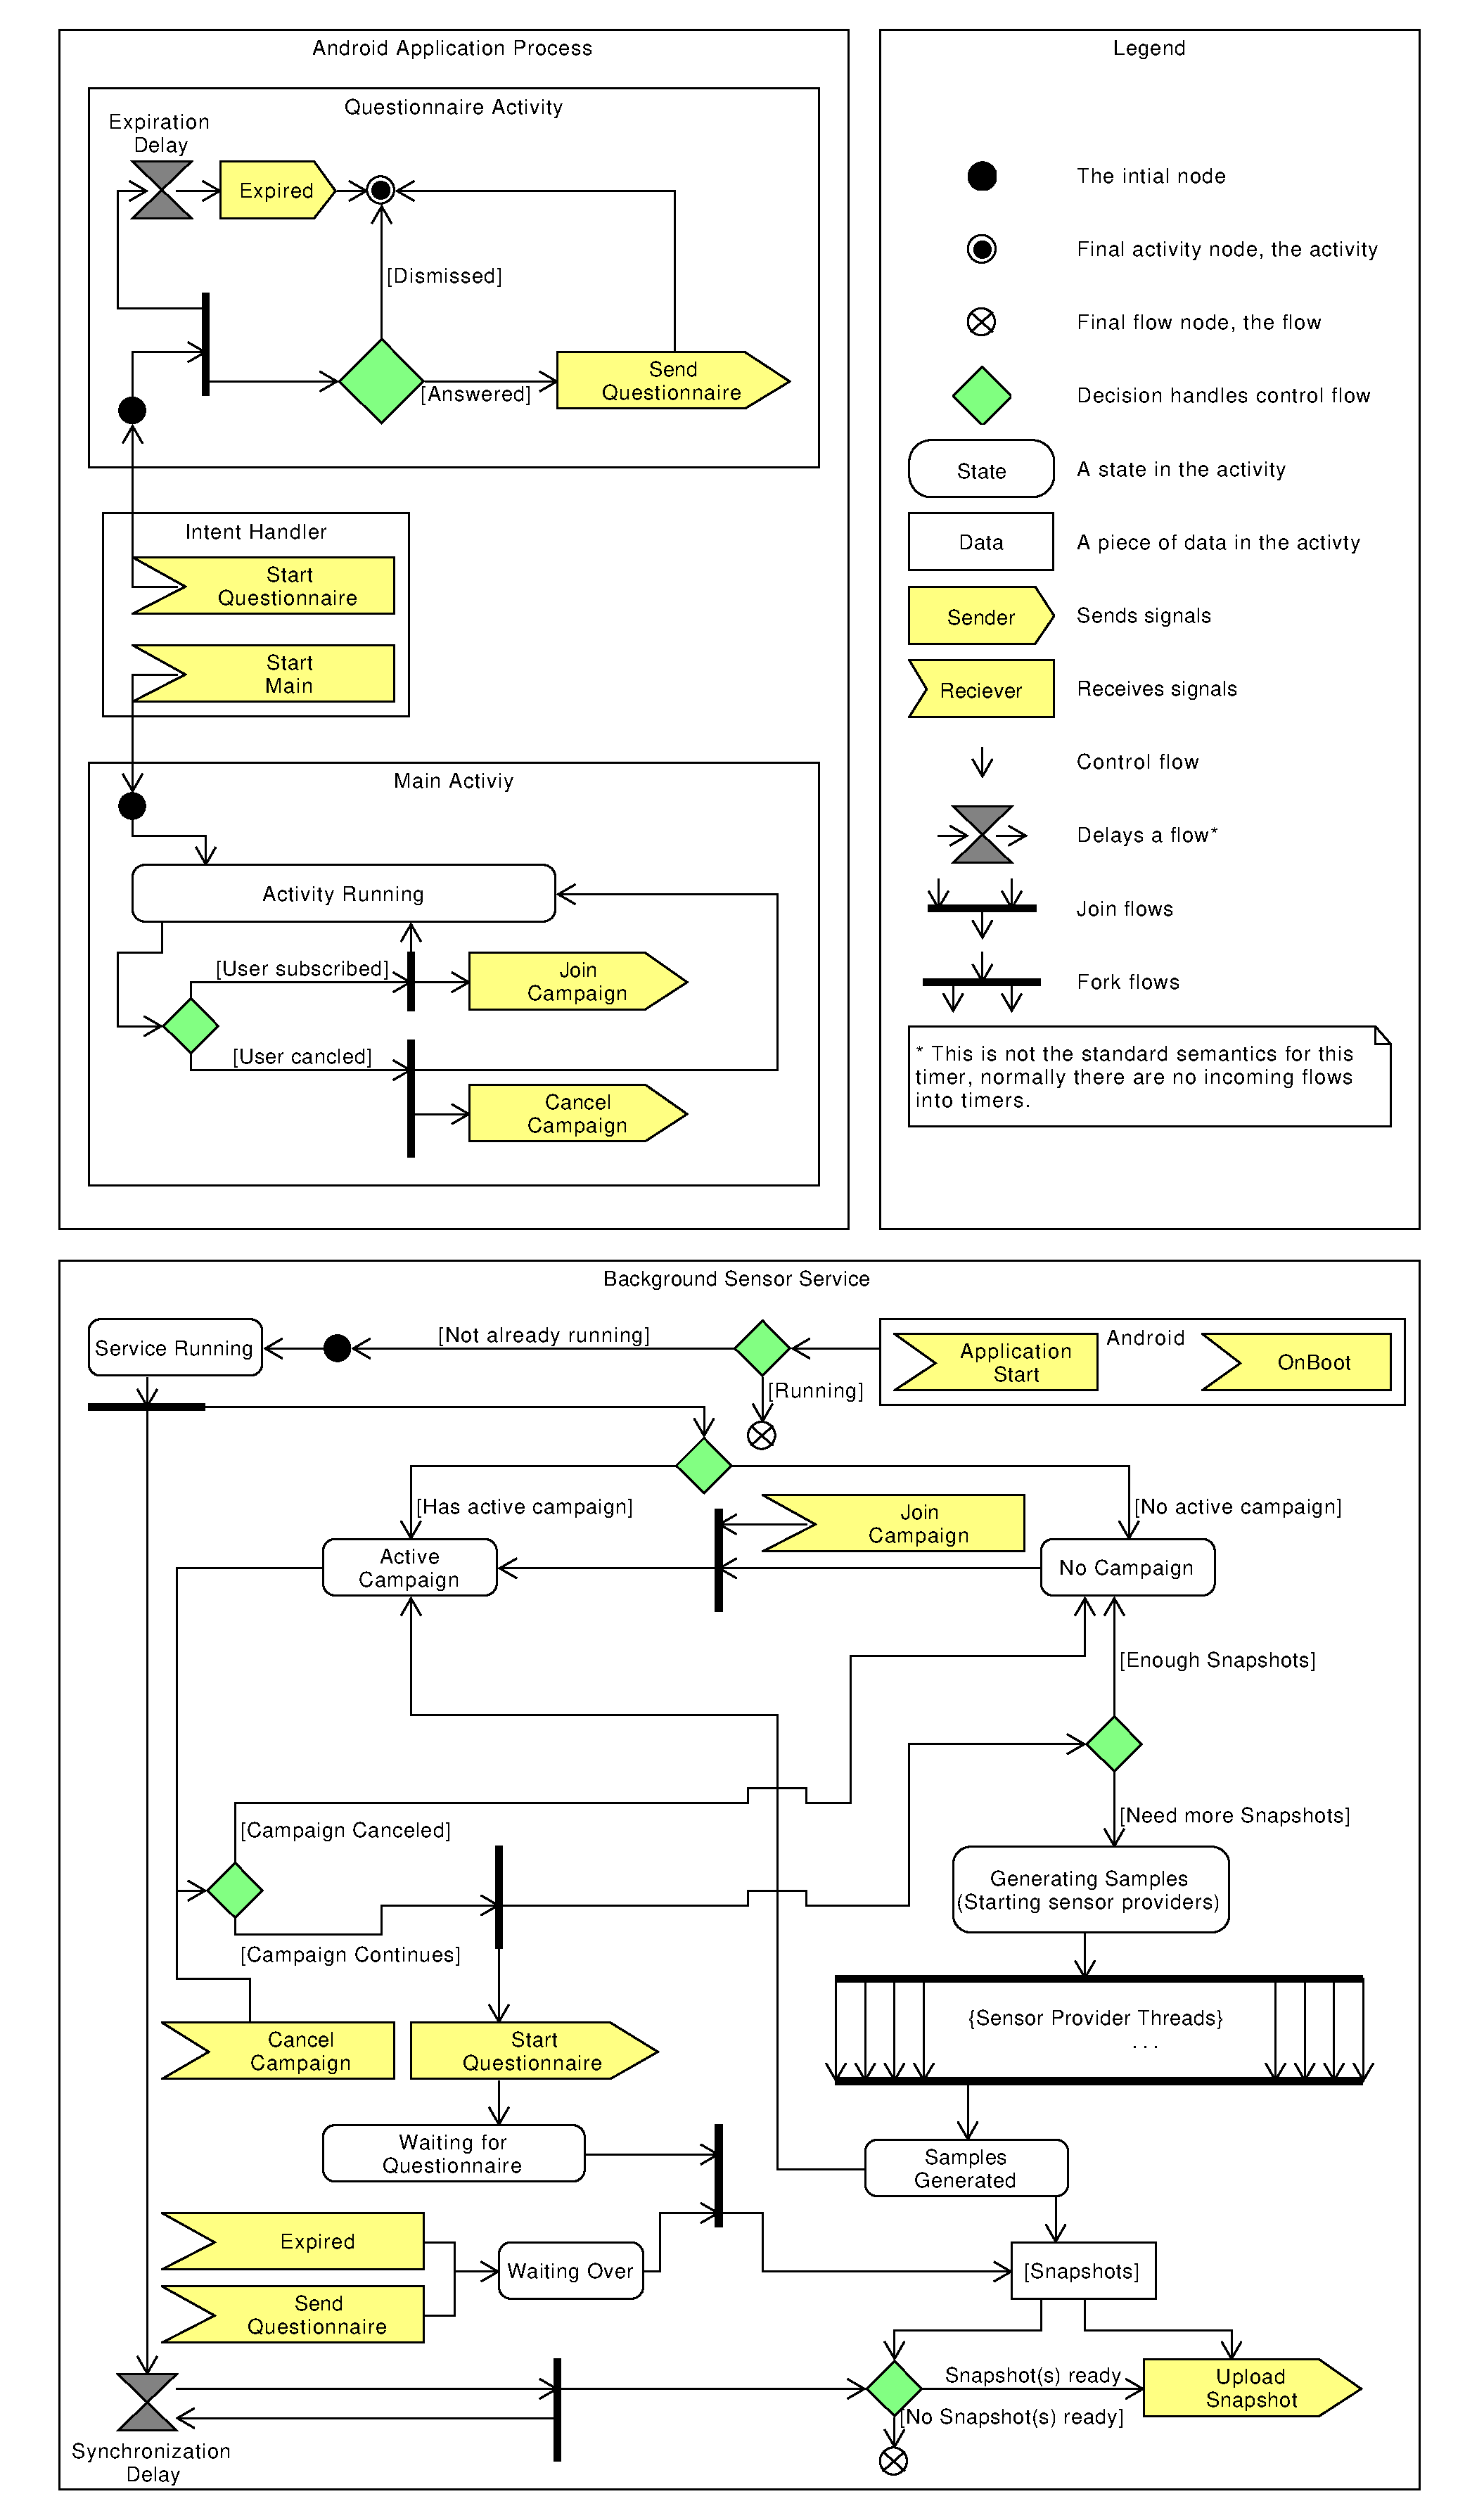
\includegraphics[width=\textwidth]{graphic/backgroundsensorservice/lifecyclestuff.pdf}
    \caption{An Activiy Diagram like overview of the mobile Application Components.}
    \label{fig:system_currency_and_lifecycle}
\end{figure}
\FloatBarrier

%!TEX root = ../../super_main.tex

\section{Compression}
\label{sec:compression}

As described in \secref{sec:data_quantity_estimation}, we would like keep the power consumption of our application low. One way of doing this is ensuring that the amount of data sent from our application to our server is the minimum amount necessary, because sending less data costs less power. During the development we discovered that many of the data types used for sensor measurements have significant overhead, compared to what is necessary in order to store the data, which opens up for the possibility of compressing the data. 
\\\\
An example of this is the heart rate sensor in the Microsoft Band 2 wearable, which uses an signed integer in order to store a heart rate. A signed integer is typically 32 bits, and has a maximum value of $2^{31} - 1$ (2,147,483,647), while a heart rate over 250 is very abnormal. This knowledge would allow us to exploit the limited value range, and use as little as 8-10 bits (values 255-1023). This would effectively cut off the majority of bits used to store a value. Furthermore, Microsoft Band 2 also uses a boolean to represent if the reading is precise (they call it locked), which uses 8 bits. This effectively means that even if you use 10 bits for the heart rate, and 1 for the locked state, you would still save 29 bits.    
\\\\
There are many more cases like that in the sensor readings, and we decided to implement a strategy for compressing one of the common values returned by many sensors, namely an array of floats containing three values. An example of a sensor that returns such measurements is the accelerometer which measures how the phone moves on its $x$, $y$, and $z$ axes. We designed a class called \mono{FloatTripleMeasurement} which is used to compress these three values to a single \mono{long}, meaning we convert $12$ bytes ($3$ floats $\times 4$ bytes) to be stored in $8$ bytes. We do this by sacrificing some of the precision of a regular float, because we think the regular precision is overkill, both in terms of sensor inaccuracy and also its usefulness for the customers. When compressing, we assume that the integer part (of the float) does not exceed $7$ numbers. We do this because the sensors only produce values ranging from $-360$ to $360$. We strip the decimal separator from the floats and treat them as a $20$ bit integer value, where the first bit determines whether the value is positive or negative. This means that we now use $60$ bits for storing the compressed value of the floats. We use the remainder of the long to add 3 bits for representing where the decimal should be placed. A visualization of the method used to compress floats can be seen in \figref{fig:float_triple_convert} and \figref{fig:float_triple_bit} respectively.

\begin{figure}[!htbp]
    \begin{alignat*}{6}
       &8.138   &&                   &&   && 8138  &&                   && \text{\mono{00000001111111001010}} \\
      -&12.821  && ~~ \rightarrow ~~ && - && 12821 && ~~ \rightarrow ~~ && \text{\mono{10000011001000010101}} \\
       &42.4878 &&                   &&   && 42487 &&                   && \text{\mono{00001010010111110111}} 
    \end{alignat*}
    \caption{Compression of floats.}
    \label{fig:float_triple_convert}
\end{figure}
\FloatBarrier

\begin{figure}[!htbp]
    \centering
    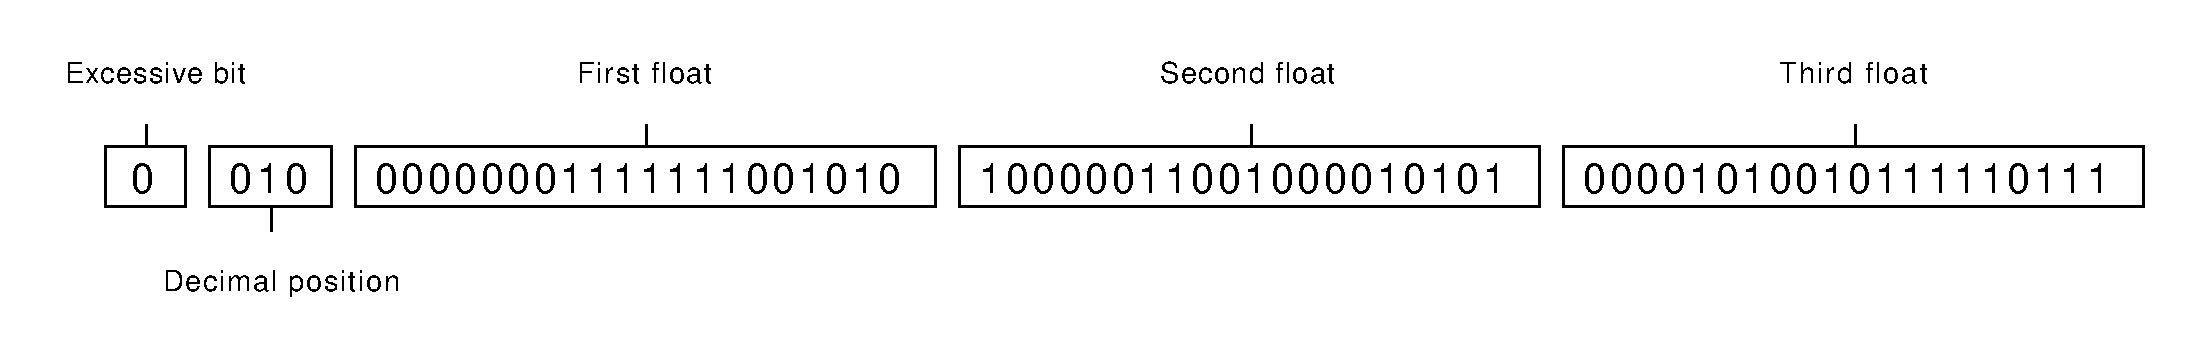
\includegraphics[width=\textwidth]{graphic/gathering_sensor_data/float_triple_bit}
    \caption{The bit representation of a \mono{FloatTripleMeasurement}.}
    \label{fig:float_triple_bit}
\end{figure}
\FloatBarrier

We wanted to compress the floating point values of the sensors so that the size of the data we need to send over network and store on the device would decrease. However, this compression does not come for free. We actively make a trade off between size of data stored and CPU cycles used for compressing and decompressing the values. We have conducted a performance test for our compression of floats that investigates how much extra time has to be spent on compressing and decompressing the floats. In the test we create a number of arrays that each contain three float values. The actual test is how fast the three float values can be multiplied together. We do this in two ways: One where we compress and decompress the float values first, and another one where we just multiply. This can give us an indication of how much time is lost on the compression when performing another task. The results of the test can be seen in \tabref{tab:results_of_compression_test}.

\begin{table}[!htbp]
\centering
    \resizebox{\textwidth}{!}{%
        \begin{tabular}{|l|l|l|l|l|l|l|}
            \hline
            ~ & \multicolumn{3}{|c|}{1+ One} & \multicolumn{3}{|c|}{Nexus 5 } \\ \hline
            Count    & \begin{tabular}[c]{@{}l@{}}With \\ compression\end{tabular}  & \begin{tabular}[c]{@{}l@{}}Without\\ compression\end{tabular} & Ratio & \begin{tabular}[c]{@{}l@{}}With \\ compression\end{tabular}   & \begin{tabular}[c]{@{}l@{}}Without \\ compression\end{tabular} & Ratio \\ \hline
            10000   &   83 ms   &   11 ms   & 7.55  &   77 ms   &   10 ms   & 7,70  \\ \hline
            100000  &  635 ms   &  172 ms   & 3.69  &  783 ms   &  113 ms   & 6,93  \\ \hline
            1000000 & 9088 ms   & 1333 ms   & 6.82  & 8245 ms   & 1090 ms   & 7,56  \\ \hline
        \end{tabular}%
    }
    \caption{Results of compression test}
    \label{tab:results_of_compression_test}
\end{table}
\FloatBarrier

As can be seen in \tabref{tab:results_of_compression_test}, it generally took seven to eight times as long to perform the multiplication when we used compression and decompression. It is, based on these results, pretty obvious that rather many CPU cycles will have to be spent on this. With this in mind, one has to consider if these extra CPU cycles, extra battery usage, etc, is worth the tradeoff. On one hand, it is possible to spend additional CPU cycles, and thereby power, before storing data on the device, in order to save $\sim 33\%$ of the space, while having to transfer less data to the server and thereby spending less power and CPU cycles on this. On the other hand we could save all the power before storing, just save the normal floats in the database, and then have to spend extra power for transferring because there is simply more data. We do not know if our approach uses more power than simply not doing it, but if the system should be expanded into something large scale, it should definitely be tested. One thing that we can definitely know for sure is that our approach uses less disk space, which is also something to consider. 
\\\\
There are furthermore the considerations of how modern compression algorithms will handle our single long compared to the three floats. In Android the standard class for sending HTTP requests has the possibility of automatically compressing requests to a format called gzip. To see if this compression would further reduce the space of the collection information, we conducted a small test, where we compressed (using gzip) some snapshots containing \mono{FloatTripleMeasurement}s, and compared them to compressed (also using gzip) snapshots containing regular floats. Note that both the snapshots were serialized using JSON, similar to what is outputted by the server, as seen in \lstref{lst:snapshot_json_example}. When compression with the gzip program, you may specify how fast the algorithm should perform the compression. The faster you specify, the less compression would be achieved. We conducted a test where we would compress using the \mono{fast} setting, but also the \mono{best} setting (slowest). The result of the conducted test can be seen in \tabref{tab:gzip_compression}. All sizes are measured in bytes.

\begin{table}[!htbp]
\centering
\begin{tabular}{r|l|l|l|}
\cline{2-4}
                                                                           & \textbf{No gzip} & \textbf{Fast gzip} & \textbf{Best gzip} \\ \hline
\multicolumn{1}{|r|}{\textbf{Size with \mono{FloatTripleMeasurements}}}    & 101,543          & 40,532             & 38,358             \\ \hline
\multicolumn{1}{|r|}{\textbf{Size with regular float measurements}}        & 118,660          & 44,893             & 38,643             \\ \hline
\multicolumn{1}{|r|}{\textbf{Difference}}                                  & 17,117           & 4,361              & 285                \\ \hline
\end{tabular}
\caption{gzip float compression test result. All sizes are in bytes.}
\label{tab:gzip_compression}
\end{table}
\FloatBarrier

This test indicates, as expected, that the biggest size difference is when not using gzip. However, when using the \mono{fast} setting, gzip will further compress the data to $\sim 38-40\%$ of the original size, and here we still see a $\sim 10\%$ difference in the size of two snapshots, indicating that using both compression methods would yield a noticeable result. When using the \mono{best} setting, the data is compressed to $\sim 33-38\%$ of the original size, however, here there is not a big difference ($\sim 1\%$) between the two snapshots, indicating that if we use the \mono{best} setting, we would not gain much in term of size. Keep in mind that this test only contains \mono{FloatTripleMeasurement}s, and might yield a much better result, when using other uncompressed measurements such as simple integers, which are used for heart rate measurements. This effectively means that using gzip is a good idea for minimizing the network impact that our solution have. We have not implemented the use of gzip in the current implementation of the system due to limited time. It is also important to keep in mind that the knowledge we have regarding the measurements will allow us to make compression methods that potentially are faster (in terms of CPU cycles) compared to gzip, which first need to find these patterns in the data. 

% It is therefore important to take into consideration when deciding whether or not to use our own compression, that the transfer gain is rather low. We use knowledge about the data we collect, while gzip utilizes patterns, and we do not know if there there is much to gain if we use this for all the different types of data we gather. There are furthermore the considerations about how fast we can compress our smaller data types compared to the normal implementation, which directly translates into the amount of necessary CPU cycles and thereby also power, which should therefore be checked before making a final decision about which solution is best. As a temporary solution, until the proper analysis has been made, we have decided to not use gzip, because it would too long time to implement on the server side without the guarantee that it would be better, and because we always transfer data on Wi-Fi anyway. 


% === DATA MODELING === %
%!TEX root = ../../super_main.tex

\chapter{Data Modeling}
\label{cha:data_modeling}

\todo[inline]{Write introduction}

% Campaign
%!TEX root = ../../super_main.tex

\section{Campaign}
\label{sec:campaign}

% Write introduction and motivation for campaign
AndWellness had a concept of campaigns \secref{sub:start_configuration} which we liked. We think we could introduce something similar to their campaigns in this project. Our concept of a campaign and its model will be known as a \textit{campaign specification}, it includes questionnaire specifications, snap shot specifications, and trigger specifications \todo{Overvej om vi skal have triggers med}. The details of our \textit{campaign specification} is further described in this section. This \textit{campaign} model will have to coexist server side and client side in order to enable customers to specify campaigns and user devices to subscribe to them.  

\subsection{Questionnaire Specification Model}
\label{sub:questionnaire_model}
We had come to the conclusion that customers should be able to define questionnaires to be a part of the data collection \secref{sec:human_activity_recognition}. Customers should be able to define one or more separate questions or more generally data inputs which combined should make out a questionnaire model. 
\\\\
Simple boolean yes/no questions can directly be combined to create a discrete amount of labels or classes which can later be used as targets for an AI model but more open inputs, which for instance can be used for regression or as more diverse features, should also be possible \todo{Overvej om vi når at implementere continuous inputs}. 
\\\\
A questionnaire specification should be transformable to a format which can be easily be parsed and send from the server to the collecting devices. We have therefore implemented a questionnaire to be Java \mono{Parcelable}. \todo{Overvej at ændre det her hvis vi gør det til JSON ting i stedet} 

\todo{Overvej om den figur skal opdateres med muligheder for mere advancerede input}
\begin{figure}[!htbp]
	\centering
	\includegraphics[width=0.6\textwidth]{graphic/data_modeling/questionnaire.pdf}
	\caption{The model of the questionnaires in the system}
	\label{fig:questionnaire_model}
\end{figure}
\FloatBarrier


\subsection{Class Diagram}
\label{sub:class_diagram}

Questionnaires are not the only source of data and different configurations of the different available sensors should also be customizable for customers. They should be able to specify which data sources they want to include, when they want the data gathered, and how much data they want at a time. 

\todo{figure out where to place this}
\begin{figure}[!htbp]
    \centering
    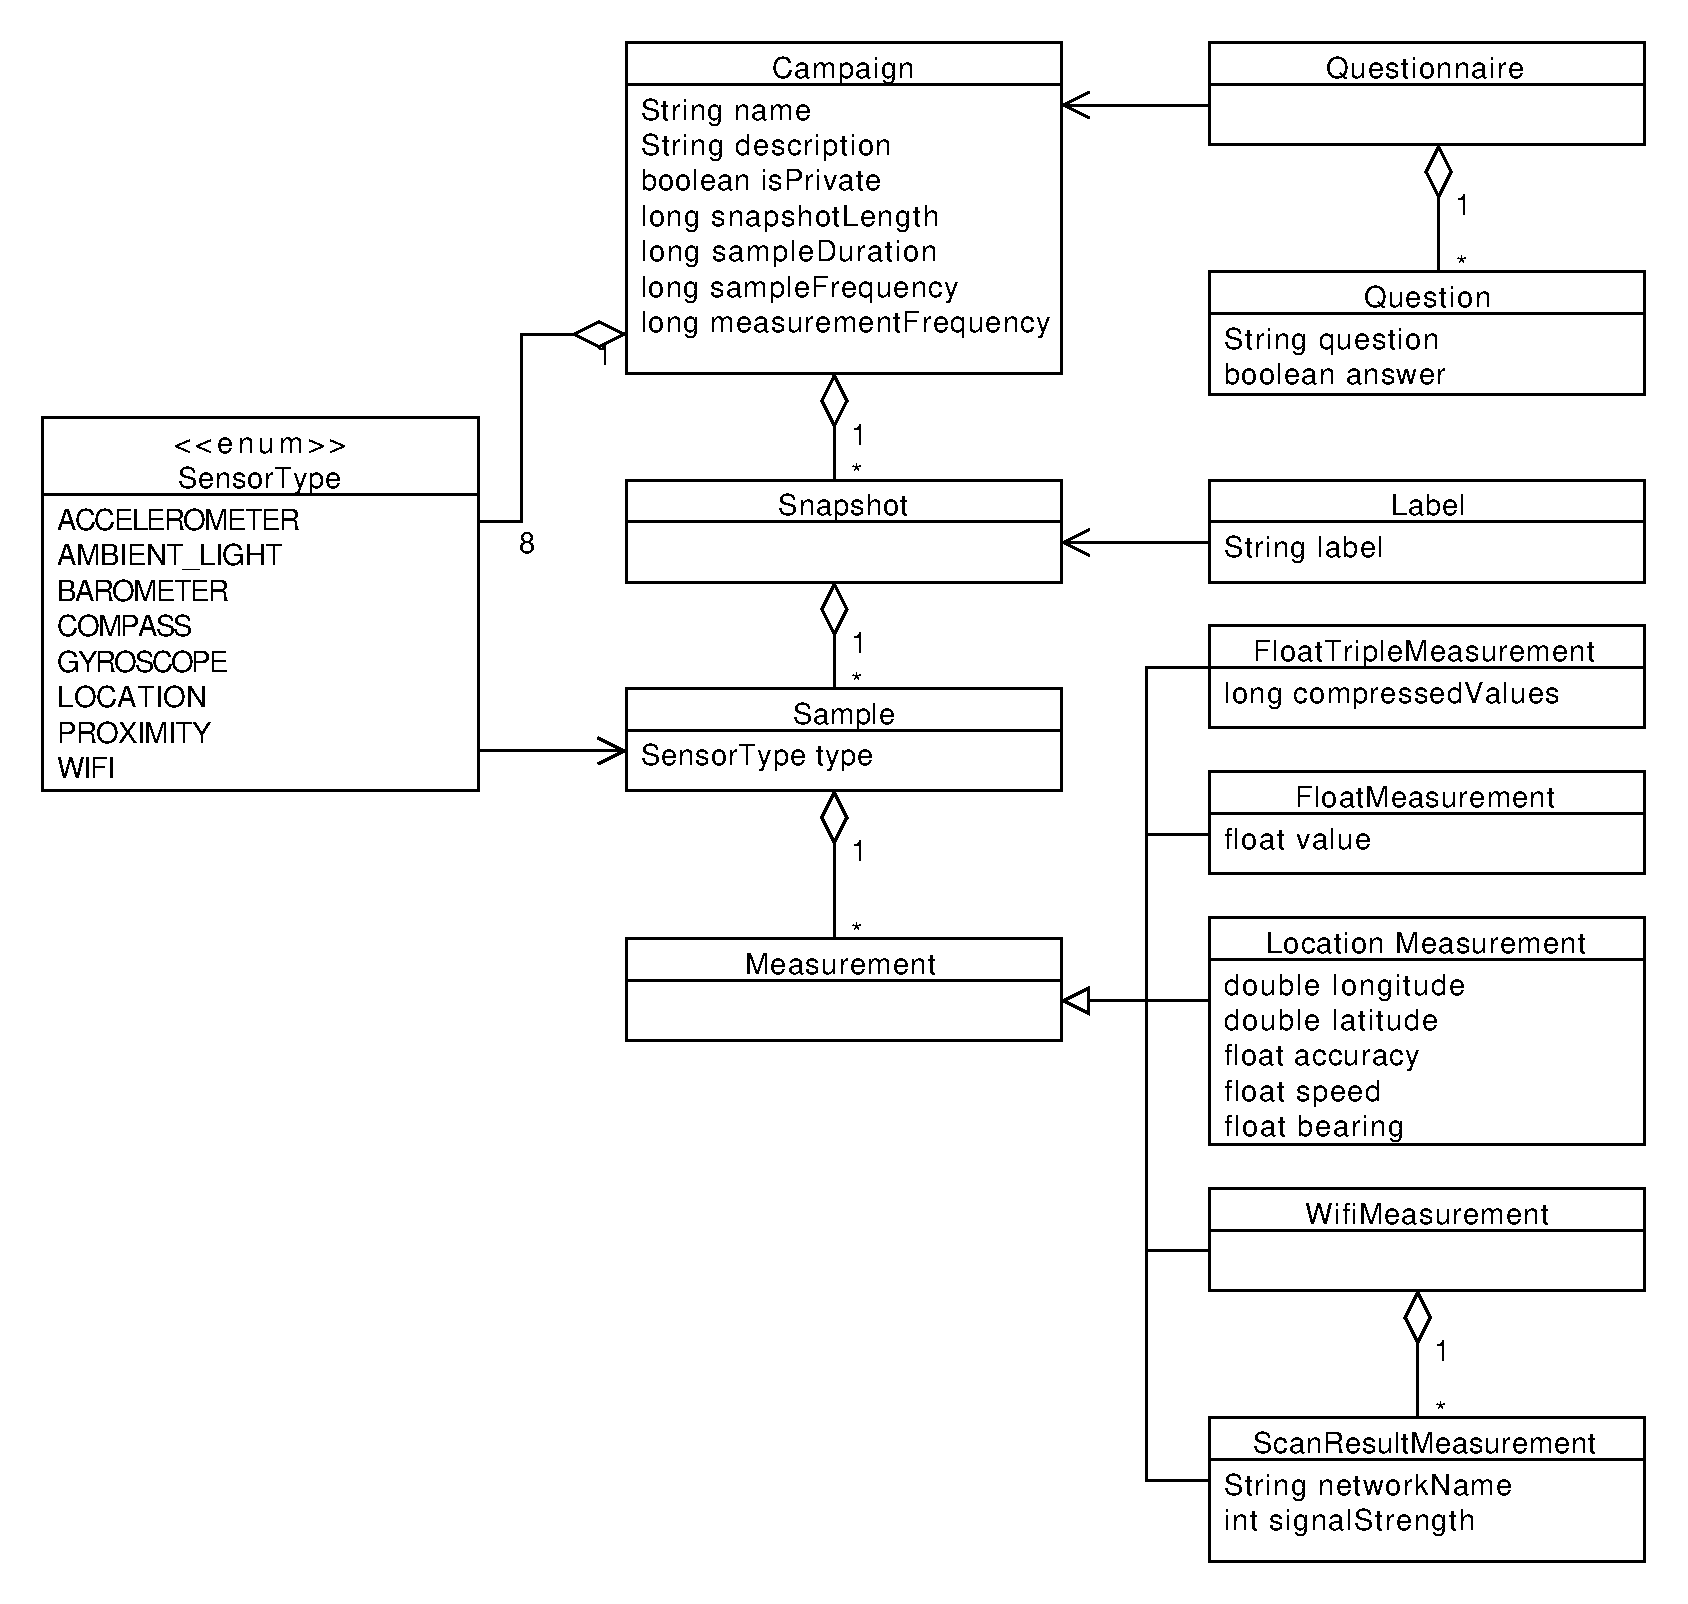
\includegraphics[width=\textwidth]{graphic/data_modeling/model_class_diagram.pdf}
    \caption{Class Diagram of the campaign model.}
    \label{fig:model_class_diagram}
\end{figure}

\todo{Slut af med at vi er kommet frem til at vi skal bruge en model for det data der er blevet indsamlet og lav forward ref til snapshot sektion}




% === CLIENT SERVER === %
%!TEX root = ../../super_main.tex

\chapter{Client Server Architecture}

A core features of the platform is that multiple clients should feed the server with data gathered from various context alongside labels that is derived form questionnaires. The way we handle this communication on both the client and the server is described in this chapter.

%!TEX root = ../../super_main.tex
\section{Consumption of Battery and Disk}

As mentioned in SECTION\todo{ref to good engineering practices}, we do not want to reactivate the network antennas repeatedly. At the same time we do not want the client application to be hardly dependent on network. Instead of streaming the data gathered from the senors directly to the server we store it persistently on the device in order to send it in bulks whenever the antennas is already active. By doing this we save a lot of battery time, in fact the larger bulks we send to the server the more energy is saved. Also we want to avoid using the cellular communication when uploading the data for two reasons. One is that this type of communication is charged per byte sent from the user, and secondly this type of communication is slower and for that reason requires the antennas to be active for longer periods of time, hence consuming more battery. If we try to utilize the WiFi as much as possible and at the same time send the data in as big chunks as possible we save energy, however we do not want to occupy the disk capacity of the device entire if the campaign is intended to gather a lot of sensor data rapidly. For this reason we have designed some rules that tries to decrease the battery consumption while still guaranteeing that the disk of the device is not overflown with sensor data.

\todo{When we have designed this, write it here!}



% === USER INTERFACE === %
%!TEX root = ../../super_main.tex

\chapter{User Interfaces}
\label{cha:user_interfaces}

% === QUALITY ASSURANCE === %
%!TEX root = ../../super_main.tex

\chapter{Quality Assurance}
\label{cha:quality_assurance}

This section describes the different measures we have used in order ensure the quality of our developed product 
\\\\
\todo{Write more intro to QA}. 
When we executed tests that required that we run the code om some device, we always attempted to run it on multiple different devices in order to support several different hardware configurations and also that we are compatible with multiple Android versions. The phones we have available all run stock Android versions from the Android open source project. This might indicate that we also cover additional OS versions that are based on the stock versions, since if we find some bug when we test against the stock version, it is most likely also present in the modified version. 

%!TEX root = ../../super_main.tex

\section{Continuous Integration}
\label{sec:continuous_integration}
As mentioned in \secref{sec:extreme_programming}, we wanted a Continuous Integration (CI) server in order to ensure that our code base always was at a stable state. We installed Jenkins on the same server that makes up the server part of our client-server architecture because it was easily available. Jenkins is an open source automation server, which supports various different plugins that helps with builds, viewing test results, etc. We configured this Jenkins server to be notified whenever our Git version control code repositories (hosted on GitHub) for both Android and PHP code were changed. When this notification happened, Jenkins would build the corresponding project and automatically run its unit tests. Whenever the build projects would go from a previously successful build to a now failing build or vice versa, the Jenkins system would send out mails to our group, so we were aware that something went wrong or that it was now fixed again. If a build failed, the mail would contain information regarding which tests failed, and their stack trace. This made it possible for us to give immediate attention to issues that we did not catch before pushing our content to the version control. \figref{fig:jenkins_front_page} shows the front page of the Jenkins website. In the left side, the build queue can be seen, which shows if any builds are currently running. In the center, the various projects that are currently configured for the Jenkins setup can be seen. The blue circle changes to red if the most recent build was a failure, and besides that, it can be seen how long time has passed since the most recent pass, most recent failure, and how long the last build took to finish. By clicking on one of the projects, statistics can be seen for checkstyes warnings, code coverage, and test results. 

\begin{figure}[!htbp]
    \centering
    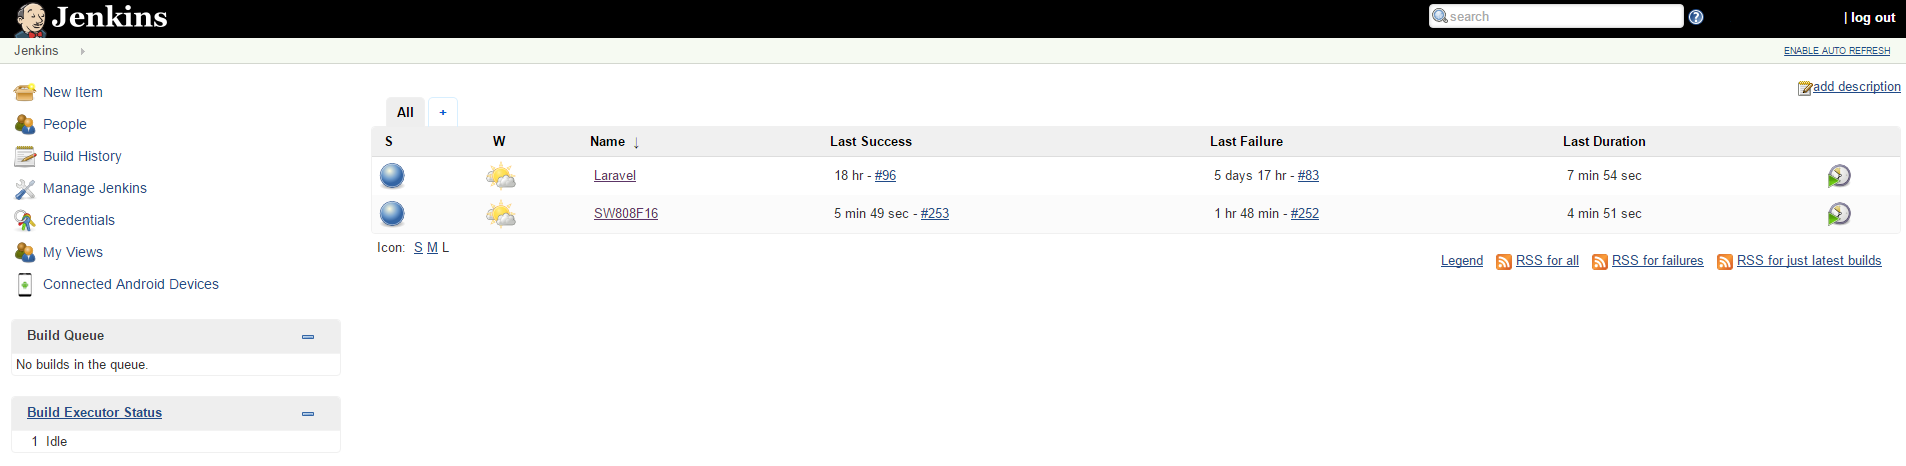
\includegraphics[width=\textwidth]{graphic/quality_assurance/jenkins_frontpage}
    \caption{Jenkins CI front page.}
    \label{fig:jenkins_front_page}
\end{figure}
\FloatBarrier

We used this extensively during the development, because when several people merge their work into the master branch of the version control several times per day, something is bound to go wrong eventually. This ensured that we always knew if something was wrong with either of our projects, so we knew when we needed to allocate people for fixing it. 


%!TEX root = ../../super_main.tex

\section{Code Metrics}
\label{sec:automated_unit_test}

Our development method states that all code we develop should be made in a test-first fashion (see \secref{sec:extreme_programming}). We therefore attempted to always make test cases for all the features we implemented. Our code coverage graphs can be seen in \figref{fig:android_project_code_coverage} and \figref{fig:php_project_code_coverage}, for our Android and PHP projects respectively. The two figures look different because we use different plugins on the CI server (due to the projects being written in different programming languages). We could have used a more strict coverage metric than line coverage, but due to prioritization of feature development we have chosen not to. Other interesting and useful coverage metrics includes branch coverage. In the Android project our line coverage percentage is $\sim 43\%$, which is relatively low. %But as explained previously, this is due to the complexity of the integration tests which were manual instead. 

% In \figref{fig:android_project_code_coverage} the line coverage is represented with green while missed lines are represented with red. In \figref{fig:php_project_code_coverage} the red line is method coverage, blue is line coverage and green is total.

\begin{figure}[!htbp]
    \centering
    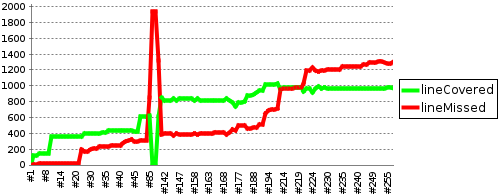
\includegraphics[width=0.7\textwidth]{graphic/quality_assurance/jenkins_android_code_coverage}
    \caption{Android project code coverage}
    \label{fig:android_project_code_coverage}
\end{figure}
\FloatBarrier

In the PHP project, we have a $\sim 74\%$ line coverage, which is rather good. Most of the untested code is library- or auto generated code, and we have not tested this because we assume these parts work as they are supposed to. This is a risk assessment we have made, and deemed insignificant, in contrast to the speed we gain from using the libraries without testing them. % If we only considered coverage on the code we made ourselves, it would probably exceed 90\%. 

\begin{figure}[!htbp]
    \centering
    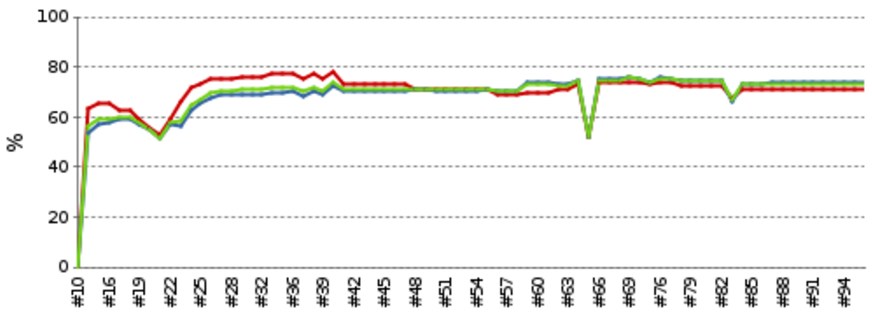
\includegraphics[width=0.7\textwidth]{graphic/quality_assurance/jenkins_php_code_coverage}
    \caption{PHP project code coverage}
    \label{fig:php_project_code_coverage}
\end{figure}
\FloatBarrier

\subsection{Manual Test}
In some cases it was infeasible to create automatic dynamic white box tests in decent time, and we therefore, in these cases, switched to a dynamic black box approach instead. Here we made test specifications, executed some part of the code manually and observed the result relative to the specifications. We mainly did this for the more complex parts of the code, such as the \mono{BackgroundSensorService} class, which schedules all the \mono{SensorProvider}s asynchronously and sends the results to the server. Here we test if the sensor provider outputs the data correctly to the server. We also used this approach for other testing methods, such as regression and integration testing of UI features. For instance, we would, when a new UI-related feature was implemented, manually test if previous UI features still worked. We did not spend time on specifying written test-cases on the most basic integration tests, such as ``is it possible to subscribe to a campaign?'', since these would probably be found during ad-hoc testing done while developing new features.
\\\\
These manual tests resulted in a generally lower line coverage, especially on the Android project, since the CI plugin we used was unable to compare our manual tests to the code base. This does not necessarily mean that the code is less tested, but it is harder to tell when tests are covering the code base well. 

\subsection{Static Code Analysis}
Besides using coverage metrics, we have used some metrics produced by static code analysis to improve the quality of our code base. We have used a linter, which will produce warnings on code that is known to be error prone, which helps us avoid common mistakes on the Android platform and Java in general. Furthermore, we have used check-style, which helps us find structural inconsistencies in our code base. Effectively, this type of metric will assist us in keeping our code base uniform and look consistent, which will make it easier for all developers to read the code, since all parts of the code base is structured in the same way.


%!TEX root = ../../super_main.tex

\section{Monkey Test}
\label{sec:monkey_test}
We executed UI/Application Exerciser Monkey tests on the android code. The exerciser monkey generates pseudo-random streams of user events, which can be used to test the robustness of the application. The monkey is able to stress-test the application because of frequent button clicks, etc., such that it most likely crashes if there are memory leaks or other bad implementations. It furthermore provides the possibility of simulating erratic user behavior, that might perform some trace of actions that human users would not typically follow, which might crash the application. Whenever the monkey crashes the application, the entire trace is available, but we mainly used it for the crash reports and exceptions that are available through the Android Debug Bridge. 
\\\\
We started by running one trace on 50000 inputs on a Galaxy Nexus phone, where the application crashed after 46000 actions, which allowed us to take a look at the exception and resolve it. Afterwards the monkey ran for 2 hours straight without crashing, and we therefore think the application is rather robust.
\\\\
Following this we also ran the monkey for a while on a Nexus 5 device which had Android 6.x, in contrast to the 5.x on the Galaxy Nexus. Here it also seemed to run without any difficulties, which gives some indication that our application is resilient in terms of different configurations and also compatible with different versions of Android without issues.
\\\\
We have also been using the monkey to discover cases where, if you executed a certain set of actions fast enough, it would would result in incorrect application behavior. This includes things such as subscribing to a campaign, immediately exiting the menu and then entering the same menu again, where the communication between application and server had not finished registering the participant yet. This allows us to find certain use patterns that we need to consider, or at least need to keep in mind, even if we do not have solutions for them at the time.
\\\\
It is also possible to configure CI servers to run automated monkey tests if so desired, but we did not think this was a good idea for our project. This was partially because it takes quite a bit of time to execute the monkey test, but also because it has access to the settings of the phone, which might mess up the unit tests. So given the amount of precautions, resets, etc., that might be necessary, we deemed it to take too much time to set up. 


%!TEX root = ../../super_main.tex

\section{Pair Group Review}
\label{sec:pair_group_review}

Two times during the project period we arranged meetings with another group of software students at Aalborg University, where we presented the current states of our projects and provided critique for each other. One meeting was arranged halfway through the semester and another was arranged three weeks before project delivery. 

\subsection{First Meeting: Project Idea}
\label{sub:first_meeting_project_idea}
The goal of the first meeting was to evaluate the general project idea of the opponent group and also suggest improvements for the developed system. At this meeting the two groups were unfamiliar with the product of the other group, so an agenda was created that should increase the understanding for the opponent:

\begin{itemize}
    \setlength\itemsep{-0.2em}
    \item Introduction
    \item Demonstration
    \item Evaluation
\end{itemize}

We took turns in presenting, so the first group started by introducing their problem area, how they were going to solve the problem and which customers might be interesting in using the developed product. After the presentation of the problem area, the group presented the current state of the product, which was followed by two different evaluations from the opponent group. One evaluation was regarding the idea and the marketability of the solution, while the other was regarding how the product could be improved. 
\\\\
The result of this meeting were mainly on the idea level, and not so much about the product specifically. Our opponent group had concerns regarding how we were going to persuade participants to use the system, such that we could actually gather the data that we claimed would be available for our customers. We decided that this was not a big concern, since the customers would be interested in branding their campaigns in order to find and persuade participants to contribute. In any case, we think that we provide a platform for customers to use, so that they only have to provide some incentive for participants to join, is an improvement in itself. We furthermore hope that the participants who join for the rewards of the branded campaigns would be interested in selecting campaigns that only offered small or no rewards. We think it is realistic to assume, that if customers do not offer any rewards whatsoever on their own without our system, they would probably not get any participants anyway. 

\subsection{Second Meeting: Product Evaluation}
\label{sub:second_meeting_product_evaluation}

At the second meeting, both the groups' products were in an nearly finished state, and were presented for the other group. The goal of this meeting was to determine if there were any obscure parts of the system, bugs, possible usability improvements or extensions to the system. Our opponent group could not find any bugs in the system, but they suggested some potential usability improvement and an extension that would be nice to have in the system. The suggestions are represented in \tabref{tab:suggestions_from_opponent_group}. 

\begin{table}[!htbp]
    \centering
    \begin{tabular}{|l|p{0.8\textwidth}|}
    \hline
    \textbf{Category} & \textbf{Description} \\ \hline
    Extension & Run questionnaires at specific times of the day, instead of relative to time of joining campaign.  \\ \hline
    Usability & Put the definition of our time intervals on the website, or show it with an image. \\ \hline
    Usability & Move the active campaign to the top of the campaigns list instead of where it was located before. \\ \hline
    Usability & Have focus on the size differences on the website. Many items are rather small, so it is hard to determine what is important. The most important things should be large. \\ \hline
    \end{tabular}
    \caption{Suggestions from opponent group.}
    \label{tab:suggestions_from_opponent_group}
\end{table}

These were all valid suggestions, but due to the meeting being held a bit too close to the project deadline, we had to prioritize documenting our work over furhter development. Effectively, this resulted in only the second entry being implemented: \emph{Put the definition of our time intervals on the website, or show it with an image}. There is now an image on the website which represents how to understand the different intervals you can specify on the ``create campaign''-site. The other three entries are things that would be nice improvements to the system, and definitely something that should be worked on, if the system was to be extended at some point. 


%!TEX root = ../../super_main.tex
\section{Participant Experience Evaluation}
\label{sec:participant_experience_evaluation}

We want uMiner to be as general as possible in terms of who participants might be. Meaning that we want to target as many different personas as possible in terms of user experience of the Android application. We have for this reason tried to create some sort of user experience evaluations in regards to the part of the system the participants are going to use. The idea of this evaluation is to determine if there are some obvious flaws in the design of how our Android application in regards to disturbing the participants. We want to investigate if we developed a solid start for part of the client application that notifies and asks the participants questions. This evaluation was performed with five people having a compatible smartphone, firstly this is not a great deal of test subjects and does not provide any statistical evidence for the evaluation of the system, but we hope to get some constructive evaluation of the application never the less. Furthermore one should not that the persona of these five test subjects are rather similar. All five are male in their start 20s, with similar interests, all being tech savvy some extend.

\subsection{Setup}
\label{sub:setup}

We have created a test campaign called ``Alcohol and you'' which should emulate the type of campaign a final customer might specify. The campaign specification can be seen in \tabref{tab:test_campaign_spec}. This specification means that we take 600 measurements every hour and we desire answers for a questionnaire every other hour.

\begin{table}[!htbp]
    \centering
	\begin{tabular}{|l|l|} \hline
	Total duration        & 2 hr                                                                                                                                                                                                                                                           \\ \hline
	Sample frequency      & 1 min                                                                                                                                                                                                                                                          \\ \hline
	Sample duration       & 2 sec                                                                                                                                                                                                                                                          \\ \hline
	Measurement frequency & 200 mili sec                                                                                                                                                                                                                                                   \\ \hline
	Sensors               & Accelerometer, 
							Ambient Light,
							Barometer,
							Compass,
							Gyroscope,
							Location,
							Proximity,
							Galvanic Skin Response (Microsoft Band 2),
							Heartbeat (Microsoft Band 2),
	Questions             & Have you within the last hour had an alcoholic beverage?,
							Have you within the last hour had a carbonated alcoholic beverage?,
							Have you within the last hour had a strong alcoholic beverage with (more than 10\% alcohol)?, 
							Do you feel influenced by alcohol? \hline
	\end{tabular}
	\caption{Alcohol and you specification}
	\label{tab:test_campaign_spec}
\end{table}
\FloatBarrier

The application was distributed and installed on devices of test subjects, and they were guided to how they could start contributing to our test campaign. This means that this test does not in any way evaluate the main activity of the system, it only evaluates the experience of being notified by the application and prompted with questions. After the setup of the application we told the test subjects to proceed with their daily life and treat the uMiner application as any other application the might have installed from the Google Play Store. 

\subsection{Results}
\label{sub:results}
After 24 hours of the application being installed on the test participants devices we asked them a series of questions to understand the disturbance of the notifications and questionnaire throughout one day of experience. 




\part{Final Thoughts} 
\label{prt:final_ _thoughts_}


% === REFLECTION === %
%!TEX root = ../../../super_main.tex

\chapter{Reflection}
\label{cha:reflection}

% ==== METHOD REFLECTION ====
\subsection{Planning Poker Reflections}
We have discovered that planning poker, which we have used to estimate tasks in iteration planning, is more valuable to us than simply being a technique for tasks estimation. Many ambiguities in task cards were discovered automatically by estimating and having short discussions about a given task. We learned that time estimation discussions quickly transformed into discussions about the semantics of the tasks when there were significant disagreements. We embraced these discussions and found that they were great means to resolve ambiguities. Time estimation discussions, when performing planning poker, are in general timeboxed, but we allowed longer discussions when we felt that task cards should be updated in order to resolve ambiguities or if we felt that tasks should otherwise be split or clarified.
\\\\
The short iterations have assisted us to steer the project with higher accuracy between iterations. 
\\\\
Using standup meetings and pair programming, we achieved a higher level of knowledge sharing and at the same time increase the quality of the software produced\todo{Vi ved sådan set ikke noget om det her endnu, så omformuler det hvis det ikke er sandt i fremtiden}. 
\\\\
Our experience shows that a user story and an acceptance test coexist in a mutual relationship. A user story draft is usually formulated first and a draft for an acceptance is then designed. The user story and acceptance test drafts are then revised back and forth until everyone claims to have understood both and have agreed on their semantics. User stories and their corresponding acceptance tests can be seen in \appref{app:user_stories_and_acceptance_test}.

% === CONCLUSION === %
%!TEX root = ../../super_main.tex

\chapter{Conclusion}
\label{cha:conclusion}
Reality mining is an area of research focused around collecting and studying data about human dynamics. A problem that we ourselves and many others have had is the fact that such data is not easy to come by. We wanted to develop a context aware application, but were not able to find any suitable data. This project originates from these difficulties. The problem statement is reproduced here for the reader's convenience:
\\
%!TEX root = ../../super_main.tex

\textbf{What characterizes a system which allows customers to specify campaigns, and allows distributed gathering of snapshots from participants to contribute to these campaigns, and how could such a system be realized?}
\\\\
We have designed and implemented a solution, uMiner, which allows customers to create customized campaigns for collection of labeled training data. The labeled training data is returned to customers in a readable JSON format, which should allow easy conversion to a format suitable to the customer's machine learning problem or other needs. The implemented system utilize a client server architecture, where the server provides data for two different clients, namely a native Android application and a web application. The server is also used for receiving the upstream of the data gathered on the Android client, through a RESTful API that ensures that the solution is scalable. The web application is used by the customers of our system, who should be able to configure what data is collected from the Android application, but also retrieve the gathered data. The Android application is split into two parts, a front-end and a background service. The front-end is designed to allow participants to join campaigns and answer related questionnaires, which are used to label the collected data. The background service is the backbone of the data gathering. It is responsible for the automated collection of sensor data from both sensors in a smartphone and sensors in a smartband, as well as activating the questionnaires in a timely fashion.  
\\\\
We have through use of different mechanics in the Android framework implemented an Android application that enables us to gather data from multiple sensors in parallel. This along with the selected client server architecture allows for distributed gathering across multiple devices. The architecture allows us to easily add new sensors in a smartphone or wearable. We handle the problem of missing sensors by explicitly checking for their presence before requesting data from them, preventing the application from crashing if the sensor is unavailable. The data from a missing sensor is simply not included in the data returned to customers.
\\\\
Through the use of questionnaires, we have attempted to label the data gathered by our system. Customers can specify a series of zero or more binary questions, which will be asked periodically and attached to the data gathered in this period. The answers to these questions are able to serve as a label of the data gathered. Customers are able to specify these questionnaires as well as the format of the data they want collected. Customers can specify precisely which sensors or data sources they want to include, and different levels of timings for when data should be read. These timings are used for the structure that we have designed for the data. We have introduced several concepts such as \emph{snapshots}, \emph{samples}, and \emph{measurements}. These concepts are used to describe the multi-leveled structure that was implemented to capture the temporal nature of sensor data. The structure should allow the customer to gather the data that they need, but will also reduce the battery and network consumption on the participants' devices by reducing the amount of data collected. We have shown that the data that we gather can be utilized to create simple classifiers even though we structure the data in this way, indicating that it should be possible to use the data in more advanced cases.
\\\\
We have taken several measures to minimize the effect that our client application has on participants' daily lives that involves the use of smart devices. We have been concerned with the battery life of the participants' devices; the network usage; and the general disturbance that might be caused by the questionnaires that the participants have to answer. We have laid out how the efficiency, in terms of battery consumption, of the implemented application can be optimized and we have implemented some battery and network consumption optimizations, such as batching network requests and restricting uploading of the collected data, to be done using Wi-Fi instead of mobile networks. The architecture of the Android application also helps the Android operating system manage resources better, by splitting the application into a front-end and a background service. We have furthermore made some efforts to decrease the size of the gathered sensor data on the devices, by implementing a structure to handle a common data type that is measured by multiple sensors. The questionnaires are presented to the participant through Android notifications which allows the user some degree of configuration of how and when they want to be disturbed in order to answer questionnaires. % We have tested this
\\\\
The privacy of participants is maintained through various encryption techniques, such as AES and SSL. These are utilized when storing and transmitting data. This ensures that the values can never be read on the disk or during transfer, and we therefore follow most of the statutory demands imposed by the Danish Data Protection Agency. 
\\\\
In general we deem the uMiner platform to be a viable product for customers that are interested in getting access to reality mining data. By the specification of campaigns and the seamless gathering of snapshots done in a secure, resource aware and non intrusive way, we think that uMiner helps alleviate the burden of gathering reality mining data.


% We are generally satisfied with the developed product, but see some areas where further development would be beneficial.

% den prøver at løse problemet
% der er plads til forbedringer

% architectur der fungere og er let at udvide
% struktur

% === UNSORTED === %
%!TEX root = ../../super_main.tex

\chapter{Unsorted} 
\label{cha:unsorted}

%!TEX root = ../../super_main.tex

\section{Development Method}
\label{sec:development_method}

This section will describe the development method that was used in this project. We choose to use Extreme Programming (XP) \parencite{xp}, with a few changes, which will be described in this section.
\\\\
The main reason why we considered XP, was because we wanted a more concrete and test-driven method compared to other agile methods such as Scrum, which we have had experience with on previous semesters.
\\\\
Extreme Programming seemed attractive to us due to the fact that the method is test-driven. We have been lacking test and evaluation during the development of the previous semester projects, where tests and evaluation were done in an ad-hoc fashion. In an agile development method, we feel that a test-driven, or a test-first approach would help us solve this problem and achieve a more structured approach to enforce testing.
\\\\
Furthermore knowledge sharing is also encouraged in XP by using different practices such as daily stand up meetings, pair programming. For us, knowledge sharing is important, since all members of the group should have insight in the product and the report written. Using these practices, we achieved a higher level of knowledge sharing and at the same time increase the quality of the software produced \todo{Vi ved sådan set ikke noget om det her endnu, så omformuler det hvis det ikke er sandt i fremtiden}.
\\\\
Extreme Programming encourages rather short iterations in comparison to other agile development methods. These short iterations will assists us to steer the project with higher accuracy between iterations. Lastly XP also have techniques to handle uncertainty in a semi structured way, by the use of spikes, which will be used to explore areas with little to no knowledge. 
\\\\
A potential issue with Extreme Programming is that an on-site customer is required. However, this project is a student project with no paying customer or user. This means that, we must role play the on-site customer during the development. This might be challenging since we will have a hard time entering the mindset of a customer. For this reason during the iteration review and planning meetings we assign each team member roles, which they must play. This means that one team member is assigned to role play the customer during the entire review/planning meeting. Other roles include tester, developer, user. This role playing makes it easier for us as a team to prioritize story cards because one team member only have to juggle one mindset during these meetings. 
\\\\
Another issue with XP could potentially be that it does not have any built in techniques to produce a student report during development. In general XP does not encourage documentation. Documentation is only considered in XP if it gives the customer value. We will have to alter the traditional approach to include producing a student report. Another potential pitfall for using XP is the lack of quality assurance (QA) team assigned to the project. A QA team assists the development team to spot potential issues with acceptance test. Because of the fact we have not been working solely XP in previous projects we cannot evaluate the quality of acceptance test based on prior experience.

\todo[inline]{Det her er nogle at de idéer og holdninger vi har haft tidligt i projektet. Det skal reflekteres over hvad der er godt og skidt når vi kommere senere hen i projektet}

\subsection{Planning Poker Reflections}

We have found that planning poker is more valuable to us than simply being a technique for tasks estimation and thereby giving us a velocity. Many ambiguities in task cards were discovered automatically by having short discussions about estimated development time. We learned that time estimation discussions quickly transformed into discussions about the semantics of the tasks when there were significant disagreements. We embraced these discussions and found that they were great means to resolve ambiguities. Time estimation discussions, when performing planning poker, are in general timeboxed, but we allowed longer discussions when we felt that task cards should be updated in order to resolve ambiguities or if we felt that tasks should otherwise be split or clarified.  


%!TEX root = ../../super_main.tex

\section{Questionnaire Model}
\label{sec:questionnaire_model}

\begin{figure}[!htbp]
	\centering
	\includegraphics[width=0.6\textwidth]{questionnaire_model/questionnaire.pdf}
	\caption{The model of the questionnaires in the system}
	\label{fig:questionnaire_model}
\end{figure}


%!TEX root = ../../super_main.tex

\section{Vision}
\label{sec:vision}

\begin{figure}[!htbp]
    \centering
    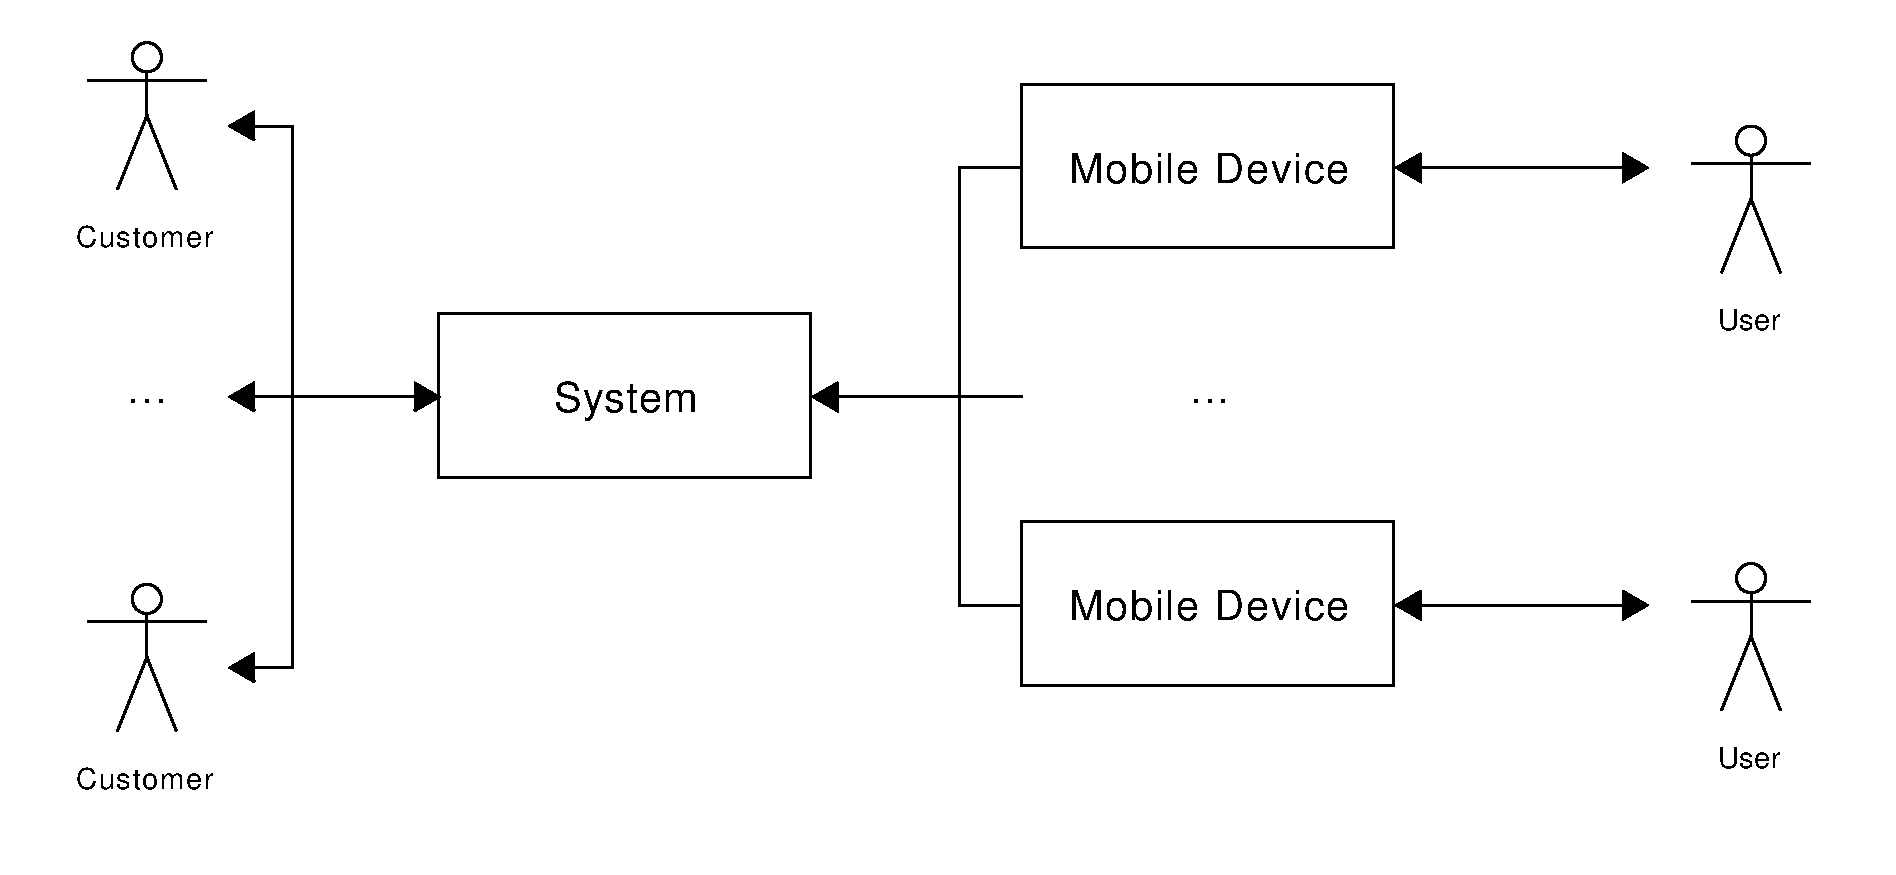
\includegraphics[width=\textwidth]{unsorted/system_vision}
    \caption{The system vision.}
    \label{fig:system_vision}
\end{figure}
\FloatBarrier


%!TEX root = ../../super_main.tex

\section{Background Sensor Service}
\label{sec:background_sensor_service}

In order to facility non-intrusive data collection in the Android system 

\subsection{What is a service?}

\subsection{Service Start}
% Boot receiver
% On Application start

\subsection{Android Service Lifecycle}




% ====================== %

% \listoftodos
% \todototoc

% === Bibliografi === %
\bookmarksetup{startatroot}
\printbibliography
\label{bibliografi}
\addcontentsline{toc}{chapter}{\numberline{}Bibliography}

% === Appendix === %
% \appendix
\part{Appendicies} 
\label{prt:appendicies_}

\begin{appendices}
%!TEX root = ../../super_main.tex

%!TEX root = ../../super_main.tex
\chapter{CD}
\label{app:cd}

\todo[inline]{indsæt de nødvendig filer og mapper}

\dirtree{%
.1 /.
    .2 Code .
        .3 \ldots.
    .2 Report.pdf.
}

%!TEX root = ../../super_main.tex

\chapter{User Stories and Acceptance Test}
\label{app:user_stories_and_acceptance_test}

All the user stories, their respective acceptance test, and which iteration they have been worked on, can be seen in \tabref{tab:user_stories_and_acceptance_test}. Because we could not complete some of the user stories in one iteration, we continued working on these user stories in the next iteration. Note that some of the user stories might sound artificial, which might be caused by that we did not have any real customer or participants, and instead chose to role-play these roles.

%!TEX root = ../../super_main.tex

\begin{center}
\begin{longtable}{| m{0.45\textwidth} | m{0.45\textwidth} |}
\hline
  \textbf{User Story}
& \textbf{Acceptance Test} \\ \hline
\endfirsthead

\multicolumn{2}{c}%
{{\bfseries \tablename\ \thetable{} -- continued from previous page}} \\
\hline
  \textbf{User Story}
& \textbf{Acceptance Test} \\ \hline
\endhead

\hline \multicolumn{2}{|r|}{{Continued on next page}} \\ \hline
\endfoot
\endlastfoot

	\multicolumn{2}{| c |}{\textbf{First iteration}} \\ \hline
	As a customer, I would like to be able to log sensor data from participants & 
	\begin{itemize}[noitemsep,topsep=0pt,parsep=0pt,partopsep=0pt]
	 	\item When you can measure and print accelerometer and gyroscope sensor data to the Android Studio log. Monitoring must be able to take place periodically and must be able to be adjusted by the programmer
	 	\item When you can measure and print the location sensor data to the Android Studio log. Monitoring must be able to take place periodically and must be able to be adjusted by the programmer.
	 \end{itemize} \\ \hline
	As a customer, I would like to get answers from questionnaires generated by me from participants & 
	\begin{itemize}[noitemsep,topsep=0pt,parsep=0pt,partopsep=0pt]
	 	\item When a customer can come up with a questionnaire, get it into the system without writing code, and have it answered by a participant.
	 	\item The questions must occur in sequence and it should only be possible to answer yes or no.
	 \end{itemize} \\ \hline
	As a developer, I would like to know how to work with sensors in Android & 
	\begin{itemize}[noitemsep,topsep=0pt,parsep=0pt,partopsep=0pt]
		\item When we know which hardware that are available and how we can communicate with them 
		\item When a section about this is written, and accepted by the group, in the report
	\end{itemize} \\ \hline
	As a developer, I would like to have a development environment & 
	\begin{itemize}[noitemsep,topsep=0pt,parsep=0pt,partopsep=0pt]
		\item When everybody in the group has installed Android Studio and it can run
		\item When continuous integration is up and running including 
			\begin{itemize}[noitemsep,topsep=0pt,parsep=0pt,partopsep=0pt]
				\item Builds
				\item Unit tests
				\item Static code analysis
				\item Code coverage
				\item Automatic builds
			\end{itemize}
		\item Code standard
		\item Version control
	\end{itemize} \\ \hline
	As a developer, I would like to know what is ethical/legally correct to log (continued to next iteration) & 
	\begin{itemize}[noitemsep,topsep=0pt,parsep=0pt,partopsep=0pt]
		\item When rules about data legislation is known about for both Denmark and Europe
		\item When a section about this is written, and accepted by the group, in the report
	\end{itemize} \\ \hline
	
	\multicolumn{2}{| c |}{\textbf{Second iteration}} \\ \hline
	As a developer, I would like to know what is ethical/legally correct to log (continued from last iteration) & 
	\begin{itemize}[noitemsep,topsep=0pt,parsep=0pt,partopsep=0pt]
		\item When rules about data legislation is known about for both Denmark and Europe
		\item When a section about this is written, and accepted by the group, in the report
	\end{itemize} \\ \hline
	As a customer, I would like to be able to log data from many participants at a time & 
	\begin{itemize}[noitemsep,topsep=0pt,parsep=0pt,partopsep=0pt]
	 	\item If we can log and save the data persistant on a remote storage from four units
	 \end{itemize} \\ \hline
	As a participant, I would like to have my data stored persistently, anonymously and secure on my device (continued to next iteration) \todo[inline]{Marhlder: Virker lidt kunstigt at participant gerne vil have de her ting med undtagelse af secure} & 
	\begin{itemize}[noitemsep,topsep=0pt,parsep=0pt,partopsep=0pt]
	 	\item If we as developers (or other students) cannot obtain the data that has been saved in four hours, without the use of our own program, password, etc.
	 	\item The storage of the data must comply with the legislation written in the report
	 \end{itemize} \\ \hline
	As a customer, I would like to have snapshots modeled in the system, where the data is compressed (continued to next iteration) & 
	\begin{itemize}[noitemsep,topsep=0pt,parsep=0pt,partopsep=0pt]
		\item When there exist a snapshot model, which does not use more than 0.42 MB storage space using all sensors (per device) for one hour
			\begin{itemize}[noitemsep,topsep=0pt,parsep=0pt,partopsep=0pt]
				\item Snapshot duration: one hour
				\item Sample frequency: one minute
				\item Sample duration one second
				\item Measurement frequency: 100 milliseconds
			\end{itemize}
	 \end{itemize} \\ \hline

	\multicolumn{2}{| c |}{\textbf{Third iteration}} \\ \hline
	As a participant, I would like to have my data stored persistently, anonymously and secure on my device (continued from last iteration and continued to next iteration) & 
	\begin{itemize}[noitemsep,topsep=0pt,parsep=0pt,partopsep=0pt]
		\item If we as developers (or other students) cannot obtain the data that has been saved in four hours, without the use of our own program, password, etc.
		\item The storage of the data must comply with the legislation written in the report
	\end{itemize} \\ \hline
	As a customer, I would like to have snapshots modeled in the system, where the data is compressed (continued from last iteration) & 
	\begin{itemize}[noitemsep,topsep=0pt,parsep=0pt,partopsep=0pt]
	 	\item When there exist a snapshot model, which does not use more than 0.42 MB storage space using all sensors (per device) for one hour
			\begin{itemize}[noitemsep,topsep=0pt,parsep=0pt,partopsep=0pt]
				\item Snapshot duration: one hour
				\item Sample frequency: one minute
				\item Sample duration one second
				\item Measurement frequency: 100 milliseconds
			\end{itemize}
	 \end{itemize} \\ \hline
	As a customer, I would like to be able to log data from many participants at a time & 
	\begin{itemize}[noitemsep,topsep=0pt,parsep=0pt,partopsep=0pt]
		\item If we as developers can log and save the data persistently on the remote storage from four devices
	\end{itemize} \\ \hline
	As a customer, I would like to be able to create campaign dynamically & 
	\begin{itemize}[noitemsep,topsep=0pt,parsep=0pt,partopsep=0pt]
		\item When you can create a campaign using a web form, have this sent to a device where it is represented on the device with a campaign name and ID
		\item When participants can join a campaign from a list
		\item When participants can join a specific campaign by specifying an ID
	\end{itemize} \\ \hline

	\multicolumn{2}{| c |}{\textbf{Fourth iteration}} \\ \hline
	As a customer, I would like to be able to specify how long a campaign should last and when a label must be determined & 
	\begin{itemize}[noitemsep, topsep=0pt, parsep=0pt, partopsep=0pt]
		\item When you can specify how long a campaign should last
		\item When you can specify in a snapshot when the participants should answer the questionnaire to determine the label
	\end{itemize} \\ \hline
	As a customer, I would like to have the participants logged data equivalent to the joined campaign &
	\begin{itemize}[noitemsep, topsep=0pt, parsep=0pt, partopsep=0pt]
		\item When a campaign is finished, and the logged data is stored persistently in the remote database where the stored data are consistent with the campaign and the user IDs matches
	\end{itemize} \\ \hline
	As a customer, I would like to be able to see the logged data from the campaigns I have created & 
	\begin{itemize}[noitemsep, topsep=0pt, parsep=0pt, partopsep=0pt]
		\item When you can obtain a JSON string from all the campaign you have created
	\end{itemize} \\ \hline
	As a customer, I would like to be able to log data from other devices than Android smartphones, especially Microsoft Band 2 &
	\begin{itemize}[noitemsep, topsep=0pt, parsep=0pt, partopsep=0pt]
		\item When you can have a snapshot which contains data from a Microsoft Band 2
	\end{itemize} \\ \hline
	As a participant, I would like to have my data stored persistently, anonymously and secure on my device (continued from last iteration) & 
	\begin{itemize}[noitemsep,topsep=0pt,parsep=0pt,partopsep=0pt]
		\item If we as developers (or other students) cannot obtain the data that has been saved in four hours, without the use of our own program, password, etc.
		\item The storage of the data must comply with the legislation written in the report
	\end{itemize} \\ \hline
	As a participant, I would like to be able to see details on the available campaigns &
	\begin{itemize}[noitemsep,topsep=0pt,parsep=0pt,partopsep=0pt]
		\item When a participant can see using his smartphone the following:
		\begin{itemize}[noitemsep,topsep=0pt,parsep=0pt,partopsep=0pt]
			\item Name and description of the campaign, 
			\item Name of the author (the customer) of the campaign
			\item Which sensors that will be used
			\item Number of measurements
			\item Which questions that will be asked
		\end{itemize}
	\end{itemize} \\ \hline

	\multicolumn{2}{| c |}{\textbf{Future iteration}} \\ \hline
	As a customer, I would like to log the use of the mobile phone such as:
	\begin{itemize}[noitemsep,topsep=0pt,parsep=0pt,partopsep=0pt]
		\item Screen usage 
		\item Network usage 
		\item Calls/SMS
		\item Audio
	\end{itemize} & 
	\begin{itemize}
		\item When screen-, network- and calls/SMS-usage and audio level can be saved in a snapshot
	\end{itemize} \\ \hline
	As a customer, I would like to specify hardware requirements on the participants devices &
	\begin{itemize}[noitemsep,topsep=0pt,parsep=0pt,partopsep=0pt]
		\item When a customer can specify which sensors that are required, and the participants cannot see campaigns which they do not have the required sensors for
		\item Participants cannot join a specific campaign if their device do not have the required sensors
	\end{itemize} \\ \hline
	As a participant, I would like to be able to adjust when to synchronize with the remote storage &
	\begin{itemize}[noitemsep,topsep=0pt,parsep=0pt,partopsep=0pt]
	 	\item When a participant can, using a preference panel, set when to synchronize by specifying the following:
	 	\begin{itemize}[noitemsep,topsep=0pt,parsep=0pt,partopsep=0pt]
	 		\item Which network types that may be used
	 		\item If the phone must be charging
	 		\item The minimum power of the device before synchronizing
	 	\end{itemize}
	 \end{itemize} \\ \hline
	 As a customer, I would like to have that at least 80\% of the participants will not be disturbed by participating a campaign &
	 \begin{itemize}
	 	\item When at least four out of five participants, we have asked to try to test our Android application for 24 hours, does not feel disturbed using our application
	 	\item The following question will be asked to the participants:
	 		\begin{itemize}
	 			\item Did you find it inconvenient to answer the questionnaire?
				\item How many times did you dismiss the notifications?
					\begin{itemize}
						\item Why?
					\end{itemize}
				\item Did you at any point desire to disable the notifications or uninstall the application entirely?
	 		\end{itemize}
	 \end{itemize}
	 \\ \hline
\caption{User stories and acceptance test.}
\label{tab:user_stories_and_acceptance_test}
\end{longtable}
\end{center}




%!TEX root = ../../super_main.tex

\chapter{Manual Test}
\label{app:manual_test}

This appendix contains the list of the manual test we have executed to maintain regression and integration testing of the entire platform. These test are dynamic black box tests, meaning that when ever a test fails some effort is needed in terms of debugging to establish why this particular test fails. 

\subsubsection{gcm-registration-and-notification-test}

\begin{enumerate}
    \item Install the application on an Android device
    \item Launch the application and watch the Android device for 60 seconds
    \item Check logcat with the tag ``GCM Registration''
        \begin{enumerate}
            \item If you see the ``GCM Registration Failed!'' message the test fails.
            \item If you see the ``GCM Registration Success'' message continue to step 3.
            \item If the 60 seconds have elapsed and none of the above messages have been shown the test fails.
        \end{enumerate}
    \item If you are on aau network visit
        \begin{itemize}
            \item https://dev.local.element67.dk:8000/gcm/notifyAll/PASSED
        \end{itemize}
    \item Otherwise visit
        \begin{itemize}
            \item https://dev.global.element67.dk:8000/gcm/notifyAll/PASSED
        \end{itemize}
    \item If your device get a notification with the message ``PASSED'' the test is passed.
\end{enumerate}

\subsubsection{upload-snapshot-on-wi-fi-test}

\begin{enumerate}
    \item Attach the debugger to your device (ensure you have access to Wi-Fi)
    \item Join the public test campaign named ``60SECOND\_TEST\_CAMP''
    \item Disable Wi-Fi (by activating flight mode)
    \item Check the debug logcat tag ``SynchronizationTimer''
        \begin{enumerate}
            \item See if the string ``Unable to upload without network'', if it does not, the test fails
            \item Enable Wi-Fi (by deactivating flight mode)
            \item If the string ``All campaigns were uploaded'' appears, the test is successful, otherwise it fails
        \end{enumerate}
\end{enumerate}

\subsubsection{fetch-campaign-specification-test}

\begin{enumerate}
    \item Attach the debugger to your device (ensure you have access to Wi-Fi)
    \item Click the info button (the button with an ``i'' on it) on the the ``60SECOND\_TEST\_CAMP'' campaign
    \item Check the debug logcat tag ``CampaignSpecification''
        \begin{enumerate}
            \item See if the string if the following strings is present:
                \begin{enumerate}
                        \item ``Campaign Specification Retrieved''
                        \item ``name: 60SECOND\_TEST\_CAMP''
                        \item ``description: 60SECOND\_TEST\_CAMP''
                        \item ``private: false'' 
                        \item ``sensors: [ACCELEROMETER, AMBIENT\_LIGHT, BAROMETER, CELLULAR, COMPASS, GYROSCOPE, LOCATION, PROXIMITY, WIFI]''
                        \item ``snapshotLength: 60000''
                        \item ``sampleDuration: 1000''
                        \item ``sampleFrequency: 1000''
                        \item ``measurementFrequency: 500''
                        \item ``campaignLength: 3''
                        \item ``questionnairePlacement: End of snapshot''
                        \item ``questions: 1: Er du god?,2: Er du dårlig?,''
                \end{enumerate}
            \item If all strings are present the test passes, otherwise it fails
        \end{enumerate}
\end{enumerate}

\subsubsection{test-campaign-joined-stored}

\begin{enumerate}
    \item Attach the debugger to your device (ensure you have access to Wi-Fi)
    \item Join the public test campaign named ``60SECOND\_TEST\_CAMP''
    \item Close the application
    \item Open the application
    \item Check the debug logcat tag ``SavedCampaign''
    \item See if the following log strings are present
        \begin{itemize}
            \item Campaign Specification Retrieved
            \item name : 60SECOND\_TEST\_CAMP
            \item description: 60SECOND\_TEST\_CAMP
            \item private: false
            \item sensors: [ACCELEROMETER, AMBIENT\_LIGHT, BAROMETER, CELLULAR, COMPASS, GYROSCOPE, LOCATION, PROXIMITY, WIFI]
            \item snapshotLength: 60000
            \item sampleDuration: 1000
            \item sampleFrequency: 1000
            \item measurementFrequency: 500
            \item 1: Er du god?,2: Er du dårlig?,
        \end{itemize}
    \item If all strings are present the test passes, otherwise it fails.
\end{enumerate}

%!TEX root = ../../super_main.tex

\chapter{Web Mockups}
\label{app:web_mockup}


\end{appendices}

\end{document} 